%\documentclass[12pt]{scrreprt}
\documentclass[12pt]{report} 

% language may be romanian or english (default is english)
% type may be bachelor or master (default is bachelor)
\usepackage[language=romanian, type=bachelor]{style}

\usepackage{tikz}    % Pachetul de bază pentru desene
\usepackage{amsmath} % Pentru simbolurile matematice (\sum, \sigma)
\usepackage{subcaption} % pune imagini pe aceeasi linie
\usepackage{tabularx}
\usepackage[table]{xcolor}
\usepackage{booktabs}
\usepackage{multirow}
\usepackage{makecell}
\usepackage{longtable}
\usepackage{array}
\usepackage{graphicx}
\usepackage{enumitem}

% ===== In preambul =====
\usepackage{tikz}
\usetikzlibrary{arrows.meta,positioning,shapes.geometric}

%\geometry{a4paper,top=2.5cm,left=3cm,right=2.5cm,bottom=2.5cm}
%in style
%controlling the appearance of your headers and footers
\usepackage{fancyhdr}
\pagestyle{fancy}
\lhead{}
\chead{}
\renewcommand{\headrulewidth}{0.2pt}
\renewcommand{\footrulewidth}{0.2pt}

\begin{document}

\specialization{INFORMATICĂ}	
\title{Strategii de eșantionare spațio-temporală pentru rețele neuronale 3D bazate pe spiking în recunoașterea emoțiilor faciale}					   
\author{Bubuianu Adrian-Florin}											
\supervisor{Prof. Dr. Pop Horia Florin \\ Drd. Marc Daria-Anastasia}				

%\enlargethispage{10cm}		
\maketitle

\newpage
\thispagestyle{empty}
\mbox{}
\newpage
\pagenumbering{roman} 

\cleardoublepage
ABSTRACT
\vspace{0.5cm}	
\hrule
\vspace{0.5cm}	
%\cleardoublepage

This thesis investigates the optimization of facial emotion recognition (FER) systems based on Spiking Neural Networks (SNN) through adaptive unsupervised learning and related sampling mechanisms. SNNs represent the third generation of neural network models, processing information via sparse discrete spikes rather than continuous values, offering significant advantages in biological plausibility and energy efficiency.
The theoretical foundation covers the mathematical modeling of spiking neurons (Leaky Integrate-and-Fire model), neural coding schemes (Rate Coding, Temporal/Latency Coding, Rank Order Coding), synaptic plasticity mechanisms (STDP and its variants), homeostasis via adaptive thresholding, and 3D Convolutional Spiking Neural Network (CSNN) architectures. The first stage of these models involves learning convolutional kernels, which requires sampling techniques. We thus investigate four strategies (random, bounding-box based, landmark centered, and on-off saliency) employed to isolate the Region of Interest during convolution.
Experiments are conducted on the CK+ dataset (309 sequences, 7 emotion classes) using 10-fold cross-validation. The best proposed 3D CSNN with unsupervised STDP learning and random sampler achieves a mean accuracy of 56.10\%, outperforming the homologous raw-pixel SVM baseline (36.57\%) and demonstrating that bio-inspired feature extraction encodes temporally discriminative information. An equivalent ANN with supervised backpropagation achieves 75.97\%, while a high-performance hybrid CNN-LSTM model (ResNet18 backbone) reaches 88.37\%, establishing a strong fully-supervised upper bound. Feature map and Grad-CAM analyses offer qualitative validation of the regions each model attends to for each emotion class.
The practical application, Neuro-Guardian, is a real-time clinical monitoring platform that integrates the CNN-LSTM inference engines into a hospital workflow. The system comprises a Node.js/Express backend, a React/TypeScript frontend, PostgreSQL for relational data, InfluxDB for emotion time-series, and a WebSocket–TCP bridge for live inference streaming. The alert subsystem implements a hysteresis mechanism (thresholds 70/55) and computes Distress and Pain scores from the inferred emotion probabilities to notify the attending physician of sustained negative emotional states.

\newpage

\section*{Mulțumiri}

Doresc să îmi exprim recunoștința profundă față de domnul profesor dr. Bilasco Ioan Marius de la Universitatea din Lille, Franța, din cadrul grupului de cercetare FOX, al laboratorului CRIStAL, pentru propunerea temei acestui proiect și pentru ghidarea constantă pe parcursul realizării cercetării. Implicarea sa directă și suportul esențial acordat în fiecare etapă a proiectului au fost pilonii fundamentali în finalizarea cu succes a acestei lucrări.

De asemenea, adresez mulțumiri coordonatorului meu științific, drd. Marc Daria-Anastasia, pentru îndrumarea atentă, sprijinul oferit de-a lungul întregii colaborări și pentru sugestiile valoroase care au contribuit la definirea acestei lucrări.

Totodată, exprim mulțumirile mele pentru accesul la resursele de calcul de înaltă performanță ale infrastructurii Grid'5000, utilizate în realizarea experimentelor din cadrul acestei cercetări.

\tableofcontents


\newpage
\pagenumbering{arabic}

\chapter*{Introducere}
\addcontentsline{toc}{chapter}{Introducere}  

Recunoașterea automată a emoțiilor faciale reprezintă una dintre cele mai active direcții de cercetare la intersecția dintre inteligența artificială, neuroștiință și viziunea computerizată. Aplicațiile sale acoperă un spectru larg, de la sisteme de asistență pentru persoane cu dizabilități de comunicare și detectarea stărilor afective în contexte clinice, până la interfețe om-calculator adaptive și sisteme de supraveghere a siguranței la volan.

Odată cu creșterea exponențială a volumelor de date vizuale și cu necesitatea procesării în timp real pe dispozitive cu resurse limitate, limitele energetice ale arhitecturilor clasice de tip ANN devin din ce în ce mai vizibile, deschizând calea pentru paradigme computaționale alternative.

Rețelele neuronale cu impulsuri (\textit{Spiking Neural Networks} – SNN) constituie a treia generație a modelelor neuronale artificiale și se aseamănă mult mai fidel cu mecanismele biologice ale creierului uman. În aceste modele, informația este transmisă prin trenuri de impulsuri discrete, iar neuronii se activează rar, doar atunci când potențialul acumulat depășește un prag critic. Această caracteristică de activare rară (\textit{sparse activation}) reduce drastic numărul operațiilor de calcul față de rețelele clasice și face SNN-urile ideal potrivite pentru implementare pe hardware neuromorfic dedicat, cum ar fi Intel Loihi sau IBM NorthPole, unde consumul energetic poate fi redus cu până la 75\% față de echivalentele ANN \cite{wang2022}.

\section*{Obiectivele lucrării}
Prezenta lucrare de licență are ca obiectiv central investigarea potențialului rețelelor neuronale convoluționale de tip spiking (CSNN) în sarcina recunoașterii emoțiilor faciale, cu accent pe impactul preprocesării adaptive asupra calității trăsăturilor extrase. Concret, obiectivele urmărite sunt:

\begin{itemize}
	\item \textbf{Implementarea unui simulator CSNN 3D} cu învățare nesupervizată prin regula STDP (\textit{Spike Timing-Dependent Plasticity}), capabil să proceseze secvențe video ale expresiilor faciale.
	\item \textbf{Proiectarea unui pipeline de preprocesare adaptivă} care permite eșantionarea locală, în jurul celor 68 de repere faciale, facilitând analiza dinamică a musculaturii feței pe parcursul cadrelor videoclipului.
	\item \textbf{Evaluarea comparativă} a modelului SNN propus față de un clasificator SVM pe pixeli bruți, un ANN echivalent cu \textit{backpropagation} supervizat și o arhitectură hibridă CNN-LSTM.
	\item \textbf{Dezvoltarea aplicației Neuro-Guardian}, un sistem clinic de monitorizare în timp real pentru urmărirea stărilor emoționale ale pacienților internați.
\end{itemize}

\section*{Contribuții proprii}
Contribuțiile originale ale prezentei lucrări includ: 
\begin{enumerate}
	\item Proiectarea unui pipeline de preprocesare adaptivă bazat pe repere faciale, cu trei strategii de eșantionare (aleatorie, \textit{bounding-box} și \textit{landmark-centrată});
	\item Studiul comparativ sistematic între patru paradigme de clasificare pe același set de date;
	\item Proiectarea și implementarea completă a aplicației clinice \textbf{Neuro-Guardian}, incluzând canalul de inferență în timp real prin WebSocket–TCP și baza de date time-series InfluxDB.
\end{enumerate}

\chapter*{Structura lucrării}
\addcontentsline{toc}{chapter}{Structura lucrării}

Lucrarea este organizată în opt capitole, după cum urmează:

\begin{description}
	\item[Capitolul 1 – Formularea problemei] prezintă grupul țintă vizat de aplicație și datele de intrare-ieșire.
	 
	\item[Încadrarea în literatura de specialitate] trece în revistă cele mai relevante rezultate: capacitatea rețelelor bazate pe spike-uri neuronale de a integra date multimodale, de a utiliza dinamica mișcărilor faciale pentru a detecta cu succes persoane deghizate, robustețea și puterea de generalizare când antrenarea și testarea au loc pe seturi diferite de date, respectiv consumul redus de energie.
	
	\item[Capitolul 2 – Fundamente teoretice] prezintă baza matematică: tranziția de la ANN la SNN, modelele de neuron (Hodgkin-Huxley, Integrate-and-Fire), schemele de codificare (Rate, Latency, Rank Order) și mecanismele de plasticitate sinaptică (STDP).
	
	\item[Capitolul 3 – Experimente și analiza rezultatelor] constituie nucleul experimental. Include detaliile setului de date CK+, metodologia 10-fold cross-validation și rezultatele comparative (SNN: 48.02\% vs. CNN-LSTM: 88.37\%).
	
	\item[Capitolul 4 - Neuro-Guardian] prezintă aplicația construită.
	
	\item[Capitolul 5 – Concluzii] sintetizează contribuțiile originale și direcțiile de cercetare viitoare.
\end{description}

%\addcontentsline{toc}{chapter}{Introducere}
%\addcontentsline{toc}{chapter}{Introduction}

\chapter{Motivația și formularea problemei}

\section*{Contextul general și relevanța problemei}

Expresiile faciale constituie canalul principal al comunicării afective nonverbale, jucând un rol fundamental în interacțiunea socială umană \cite{sariyanidi2015}. Sistemele informatice convenționale, însă, interacționează cu utilizatorii aproape exclusiv prin conținut verbal sau textual, ignorând în mare măsură această dimensiune esențială a comunicării.

Deficitul devine critic în contextele în care persoana nu poate sau nu dorește să verbalizeze starea afectivă:
\begin{itemize}
	\item Pacienții cu boli neurodegenerative (demență, Alzheimer);
	\item Persoanele cu tulburări din spectrul autist;
	\item Pacienții sedați sau postoperator;
	\item Copiii mici sau persoanele care nu vorbesc limba personalului medical.
\end{itemize}

În toate aceste situații, un sistem capabil să detecteze automat și în timp real stările emoționale exclusiv pe baza expresiei faciale ar constitui un instrument clinic de valoare considerabilă, permițând personalului medical să reacționeze prompt la semnale de disconfort, durere sau anxietate care altfel ar trece neobservate.

Dincolo de contextul clinic, aplicațiile recunoașterii automate a emoțiilor faciale (\textit{Facial Emotion Recognition} - FER) acoperă un spectru larg: monitorizarea atenției șoferilor, sisteme de tutoriat inteligent, analize de marketing și interfețe om-calculator adaptive pentru realitate virtuală.

\section*{Formularea problemei}

Problema abordată în prezenta lucrare poate fi enunțată formal astfel: dat fiind un flux video al feței unui subiect uman, să se construiască un sistem automat care mapează fiecare secvență de cadre la una dintre cele șapte categorii emoționale fundamentale definite în modelul extins al lui Ekman \cite{ekman1986new, ekman1992argument}: \textit{Anger, Contempt, Disgust, Fear, Happiness, Sadness} și \textit{Surprise}.

\begin{description}
	\item[Intrarea sistemului:] O secvență de cadre video (în cazul de față, câte $10$ cadre extrase din setul de date CK+), care surprind evoluția temporală a expresiei faciale de la starea neutră până la apexul emoției. 
	\item[Ieșirea sistemului:] Un vector de probabilități al emoțiilor. În cadrul aplicației \textbf{Neuro-Guardian}, aceste date sunt agregate temporal pentru calculul scorurilor de \textit{suferință} și \textit{durere}.
\end{description}

Procesul intern investigat în cazul rețelelor neuronale bazate pe spike-uri (SNN) este descris printr-un pipeline structurat în cinci etape principale, ilustrat schematic în Figura~\ref{fig:pipeline_general}. Acesta se parcurge secvențial de la stânga la dreapta și începe cu etapa de \textbf{Input Video}, în care datele brute formate din secvențe video grayscale ($48 \times 48$ pixeli, 10 cadre/secv.) sunt introduse în sistem. În faza de \textbf{Preprocesare}, se realizează configurarea setului de date prin împărțirea în pliuri de antrenare și testare (\textit{Train+Test sequences}) și selectarea unui algoritm de eșantionare (\textit{Random, Landmark, BoundingBox} sau \textit{OnOffSaliency}). Urmează \textbf{Codificare Spikes}, etapă în care imaginile sunt transformate în reprezentări temporale sub formă de trenuri de impulsuri ($t \in [0.0, 1.0]$) prin tehnici precum filtre \textit{On/Off} și \textit{Latency Coding}. Ulterior, modulul \textbf{CSNN 3D} extrage trăsăturile spațio-temporale utilizând convoluții 3D bazate pe învățare nesupervizată de tip STDP, inhibiție și homeostazie. În urma decodificării, hărțile de caracteristici trec printr-un mecanism de pooling \textit{spațial} și \textit{temporal}. În final, în etapa \textbf{SVM $\rightarrow$ Emoție}, clasificatorul analizează vectorul de trăsături rezultat pentru a determina distribuția probabilistică a celor șapte emoții țintă și a stabili eticheta finală dominantă.

\begin{figure}[htbp]
	\centering
	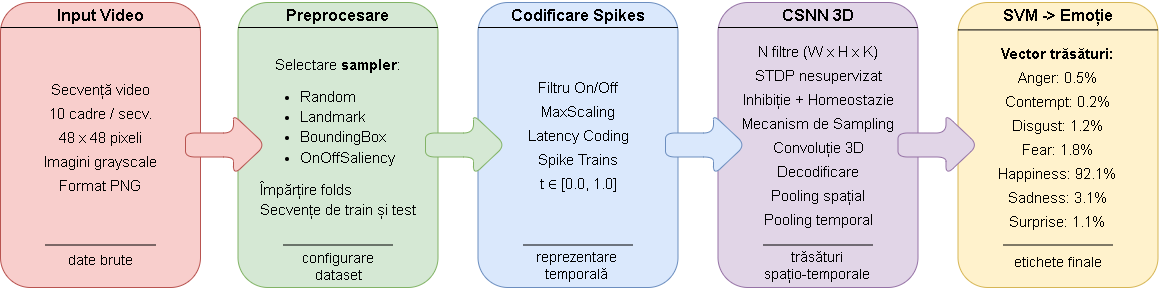
\includegraphics[width=0.99\textwidth]{figures/pipeline.drawio.png} 
	\caption{Schema bloc a sistemului propus: de la fluxul video la clasificarea emoțiilor prin SNN.}
	\label{fig:pipeline_general}
\end{figure}

\section*{Dificultatea recunoașterii emoțiilor}

Deși recunoașterea expresiilor faciale (FER) partajează cu recunoașterea obiectelor statice provocări fundamentale, precum similitudinea inter-clasă în plan static (unde elemente vizuale comune pot genera confuzii macro), specificul FER aduce o complexitate majoră determinată de natura sa intrinsec dinamică. În mod particular, FER se confruntă cu o variabilitate intra-clasă ridicată, întrucât aceeași emoție se poate manifesta prin tipare de mișcare și intensități faciale extrem de diverse de la un individ la altul. La această dificultate specifică se adaugă problema generică a dezechilibrului de clase din seturile de date academice (precum CK+), unde o distribuție neuniformă a eșantioanelor afectează direct capacitatea de generalizare în timpul antrenării. Mai mult, eficiența procesării secvențiale a fluxului video devine un criteriu critic pentru sistem; constrângerile impuse de o aplicație în timp real (precum Neuro-Guardian) cer o latență redusă per cadru, ceea ce limitează utilizarea modelelor \textit{deep learning} masive și impune soluții optimizate pentru analiza temporală. 

Deși arhitecturile clasice (CNN-LSTM) ating acuratețe ridicată (de $88.37\%$ în cadrul experimentelor realizate și descrise în Secțiunea \ref{sc:cnn-lstm}), ele implică un cost energetic substanțial prin înmulțiri matriciale continue. 

Rețelele neuronale cu impulsuri adresează această ineficiență prin:
\begin{enumerate}[noitemsep]
	\item \textbf{Activare bazată pe evenimente:} Neuronii consumă energie doar atunci când generează un \textit{spike}. În perioadele de imobilitate facială, activitatea rețelei este minimă.
	\item \textbf{Filtrarea naturală a zgomotului:} Prin filtrarea On/Off, pixelii statici din fundal nu generează impulsuri, concentrând calculul exclusiv pe zonele cu dinamică relevantă.
	\item \textbf{Codificarea temporală (\textit{Latency Coding}):} Trăsăturile proeminente produc impulsuri timpurii, creând o ierarhie temporală pe care regula STDP o exploatează pentru a învăța trăsături spațio-temporale fără a avea nevoie de etichete în faza de antrenare.
\end{enumerate}

\section*{Încadrarea în literatura de specialitate}
%\addcontentsline{toc}{chapter}{Încadrarea în literatura de specialitate}

\subsection*{Recunoașterea emoțiilor faciale folosind rețele SNN bio-inspirate}

Lucrarea elaborată de Mansouri-Benssassi și Ye \cite{mansouri2021} investighează aplicabilitatea rețelelor neuronale cu impulsuri (SNN) bio-inspirate în sarcini de recunoaștere a emoțiilor faciale (FER), punând un accent deosebit pe robustețea la zgomot și capacitatea de generalizare. Arhitectura propusă adaptează modelul Diehl și Cook \cite{diehl2015}, utilizând învățarea nesupervizată prin plasticitate dependentă de timpul impulsurilor (STDP). Procesarea imaginilor implică utilizarea filtrului Laplacian of Gaussian (LoG) pentru extracția eficientă a marginilor, urmată de o codificare de tip \textit{rate coding} prin trenuri de impulsuri Poisson, unde intensitatea pixelilor dictează rata de declanșare a neuronilor de tip Leaky Integrate-and-Fire (LIF). Modelul este structurat pe trei straturi: unul de intrare, un strat excitator (cu funcții de convoluție) și un strat inhibitor pentru selecția neuronului activ. Evaluările realizate pe seturile de date JAFFE și CK+ relevă faptul că SNN-ul obține performanțe comparabile cu metodele HOG+SVM și superioare arhitecturilor CNN pe seturi de date mici. Un aspect critic evidențiat este superioritatea SNN în experimentele de generalizare \textit{cross-dataset} (atingând până la 92\%) și reziliența remarcabilă la zgomot de tip \textit{salt and pepper}; la un nivel de degradare de 0,5, SNN menține o acuratețe de 56,2\%, depășind net modelele CNN (22,6\%) și SVM (14,1\%). Totuși, se identifică limitări privind utilizarea codificării pe bază de rată în detrimentul celei temporale și necesitatea rulării pe hardware neuromorfic dedicat pentru a maximiza eficiența energetică și computațională față de implementările actuale pe CPU/GPU.

\subsection*{Abordări bazate pe evenimente: Arhitectura Spiking-FER}

O contribuție majoră în domeniu este adusă de Barchid et al. \cite{barchid2023}, care introduc conceptul de „Event-based FER” și propun primul benchmark de acest tip prin conversia seturilor de date video clasice (CK+, ADFES, CASIA și MMI) în fluxuri de evenimente folosind simulatorul V2E \cite{yuhuang2021}. Autorii propun \textit{Spiking-FER}, o arhitectură SNN convoluțională profundă bazată pe SEW-ResNet-18, care utilizează neuroni de tip \textit{Integrate-and-Fire} (IF). Pentru a permite antrenarea de tip \textit{end-to-end} și a depăși problema non-diferențiabilității funcției de prag, se utilizează \textit{Surrogate Gradient Learning} cu o aproximare bazată pe funcția arctan. Spre deosebire de metodele modulare, abordarea \textit{end-to-end} permite optimizarea simultană a extractorului de trăsături și a clasificatorului. Rezultatele experimentale indică faptul că \textit{Spiking-FER} atinge performanțe comparabile cu modelele ANN, însă cu o eficiență energetică net superioară, fiind de până la 65,39 ori mai eficient din punct de vedere computațional. Studiul analizează, de asemenea, impactul tehnicilor de augmentare a datelor specifice evenimentelor (\textit{Event Data Augmentation}), concluzionând că metodele \textit{EventDrop} și \textit{Mirror} sunt esențiale pentru reglarea antrenării pe seturi de date limitate. Totuși, o limitare importantă a studiului rămâne dependența de date simulate în locul senzorilor DVS (\textit{Dynamic Vision Sensor}) reali și utilizarea bazelor de date de laborator, care pot să nu reflecte complexitatea emoțiilor spontane din mediul real.

\subsection*{Recunoașterea emoțiilor prin senzori de viziune dinamică simulați}

Într-o direcție asemănătoare, lucrarea propusă de Wang et al. \cite{wang2022} abordează deficitul de seturi de date pentru senzori de viziune dinamică (DVS) în recunoașterea emoțiilor prin propunerea unei metode de generare a datelor simulate din segmente video convenționale (setul CMU-MOSI \cite{zadeh2016}). Autorii introduc un cadru SNN bazat pe modelul de neuron \textit{Parametric Leaky Integrate-and-Fire} (PLIF), care permite optimizarea automată a parametrilor de scurgere (\textit{leak}) în timpul antrenării. O contribuție metodologică importantă este utilizarea unei prime rame de tip \textit{float-value} pentru a stabiliza potențialul de membrană, urmată de trenuri de impulsuri binare, strategie care accelerează scăderea funcției de pierdere și îmbunătățește a\-cu\-ra\-te\-țea față de modelele care folosesc exclusiv \textit{spikes}. Arhitectura este compusă dintr-un modul de extracție a trăsăturilor cu straturi convoluționale și \textit{average pooling}, un grup de neuroni de votare și un modul de mapare emoțională care traduce ratele de declanșare în etichete de polaritate. Antrenarea se realizează prin gradient surogat și \textit{backpropagation through time} (BPTT). Rezultatele experimentale demonstrează că modelul SNN reduce consumul de energie cu 75\% față de echivalentul ANN, atingând performanțe optime la un prag de tensiune de 0,4. Totuși, datele simulate nu pot reproduce fidel rezoluția temporală fină a unui senzor DVS real, iar constrângerea ferestrei temporale la 68 de cadre poate duce la pierderea informațiilor în cazul secvențelor video de lungimi inegale.

\subsection*{Fuziunea multimodală și arhitecturi evolutive: Modelul FusionSense}

Lucrarea prezentată de Tan et al. \cite{tan2020} introduce \textit{FusionSense}, primul sistem de recunoaștere a emoțiilor bazat pe rețele neuronale cu impulsuri care utilizează fuziunea datelor multimodale (expresii faciale corelate cu semnale fiziologice precum ECG, conductanța pielii și respirația). Autorii utilizează cadrul \textit{NeuCube} \cite{kasabov2014}, o arhitectură SNN evolutivă (eSNN) care încorporează o structură spațială 3D de tip \textit{reservoir} (3D-SNNr) cu conectivitate \textit{small-world}. Pipeline-ul vizual utilizează algoritmul Viola-Jones pentru detecție și metoda Kanade-Lucas-Tomasi (KLT) pentru urmărirea punctelor de interes, extrăgând distanțe relative între 68 de repere faciale (\textit{landmarks}) raportate la o stare neutră de referință. Un aspect metodologic distinct este utilizarea codificării de tip \textit{population coding} bazată pe câmpuri receptive Gaussiene, urmată de o învățare nesupervizată prin STDP și o etapă supervizată ce folosește reguli de tip \textit{Rank Order} (deSNN). Experimentele pe setul de date MAHNOB-HCI demonstrează că fuziunea la nivel de trăsături (\textit{feature-level fusion}) este superioară celei la nivel de decizie, atingând o acuratețe de 73,15\% pentru valența binară. Sistemul se remarcă prin capacitatea de antrenare incrementală (\textit{one-pass}), fiind optim pentru aplicații \textit{real-time}. Totuși, studiul prezintă limitări legate de excluderea semnalelor EEG și de dependența de o fereastră temporală fixă de 30 de secunde, care poate omite dinamica emoțională pe termen lung.

\subsection*{Recunoașterea identității prin dinamica mișcărilor faciale}

Lucrarea propusă de Liu et al. \cite{liu2020} introduce o paradigmă inovatoare de re\-cu\-noaș\-te\-re facială bazată pe dinamica mișcărilor musculare, metodă eficientă chiar și în scenarii cu fețe deghizate sau parțial ocultate. Spre deosebire de sistemele convenționale care se bazează pe trăsături spațiale statice, acest model utilizează cadre diferențiale pentru a captura micro-mișcările unice induse de vorbire. Arhitectura este de tip SNN profund, structurată pe cinci straturi care simulează calea ventrală a sistemului vizual biologic, incluzând module de extracție a trăsăturilor de nivel înalt prin filtre Gabor și codificare temporală bazată pe \textit{Rank Order Coding} (ROC). Un element central al modelului este stratul de învățare care utilizează mecanismul \textit{Soft Winner-Take-All} (WTA) cu inhibiție laterală și reguli STDP \textit{event-driven}, asigurând selectivitatea neuronilor pentru tipare motorii specifice. Evaluările pe setul de date MakeFaceDB au demonstrat rate de succes între 95\% și 100\%, depășind modelele CNN echivalente, în special în scenariile cu deghizări complexe (măști, barbă falsă). Autorii subliniază eficiența procesului de convergență, care necesită doar două clipuri video pentru antrenare. Totuși, sunt identificate limitări practice importante: dependența de mișcarea activă a subiectului (necesitatea de a vorbi), sensibilitatea ridicată la mișcările de fundal sau ale camerei și necesitatea unei reglări manuale riguroase a hiperparametrilor pentru a menține stabilitatea rețelei.

\subsection*{Concluzii}
Capitolul de față a stabilit cadrul general al lucrării: necesitatea clinică a unui sistem automat de recunoaștere a emoțiilor faciale, formularea formală a problemei ca mapare a secvențelor video la cele șapte categorii emoționale fundamentale ale modelului Ekman, și principalele dificultăți tehnice --- variabilitatea intra-clasă ridicată, similaritatea inter-clasă, dezechilibrul de clase și constrângerile de eficiență computațională în timp real. Totodată, analiza literaturii de specialitate a evidențiat că rețelele neuronale cu impulsuri reprezintă o direcție promițătoare, capabilă să depășească metodele clasice în scenarii de generalizare cross-dataset și de robustețe la zgomot, cu un potențial semnificativ de eficiență energetică pe hardware neuromorfic dedicat. Pornind de la aceste premise, capitolul următor prezintă fundamentele teoretice necesare înțelegerii arhitecturii propuse: tranziția de la modelele SVM, la ANN clasice și până la SNN, modelarea matematică a neuronului cu impulsuri, filtrele On/Off, schemele de codificare neurală și mecanismele de plasticitate sinaptică pe care se bazează întregul pipeline experimental, arhitecturile CSNN, metode de eșantionare și de decodificare a impulsurilor.
%\chapter*{Încadrarea în literatura de specialitate}
\addcontentsline{toc}{chapter}{Încadrarea în literatura de specialitate}

\section*{Recunoașterea emoțiilor faciale folosind rețele SNN bio-inspirate}

Lucrarea elaborată de Mansouri-Benssassi și Ye \cite{mansouri2021} investighează aplicabilitatea rețelelor neuronale cu impulsuri (SNN) bio-inspirate în sarcini de recunoaștere a emoțiilor faciale (FER), punând un accent deosebit pe robustețea la zgomot și capacitatea de generalizare. Arhitectura propusă adaptează modelul Diehl și Cook \cite{diehl2015}, utilizând învățarea nesupervizată prin plasticitate dependentă de timpul impulsurilor (STDP). Procesarea imaginilor implică utilizarea filtrului Laplacian of Gaussian (LoG) pentru extracția eficientă a marginilor, urmată de o codificare de tip \textit{rate coding} prin trenuri de impulsuri Poisson, unde intensitatea pixelilor dictează rata de declanșare a neuronilor de tip Leaky Integrate-and-Fire (LIF). Modelul este structurat pe trei straturi: unul de intrare, un strat excitator (cu funcții de convoluție) și un strat inhibitor pentru selecția neuronului activ. Evaluările realizate pe seturile de date JAFFE și CK+ relevă faptul că SNN-ul obține performanțe comparabile cu metodele HOG+SVM și superioare arhitecturilor CNN pe seturi de date mici. Un aspect critic evidențiat este superioritatea SNN în experimentele de generalizare \textit{cross-dataset} (atingând până la 92\%) și reziliența remarcabilă la zgomot de tip \textit{salt and pepper}; la un nivel de degradare de 0,5, SNN menține o acuratețe de 56,2\%, depășind net modelele CNN (22,6\%) și SVM (14,1\%). Totuși, se identifică limitări privind utilizarea codificării pe bază de rată în detrimentul celei temporale și necesitatea rulării pe hardware neuromorfic dedicat pentru a maximiza eficiența energetică și computațională față de implementările actuale pe CPU/GPU.

\section*{Abordări bazate pe evenimente: Arhitectura Spiking-FER}

O contribuție majoră în domeniu este adusă de Barchid et al. \cite{barchid2023}, care introduc conceptul de „Event-based FER” și propun primul benchmark de acest tip prin conversia seturilor de date video clasice (CK+, ADFES, CASIA și MMI) în fluxuri de evenimente folosind simulatorul V2E \cite{yuhuang2021}. Autorii propun \textit{Spiking-FER}, o arhitectură SNN convoluțională profundă bazată pe SEW-ResNet-18, care utilizează neuroni de tip \textit{Integrate-and-Fire} (IF). Pentru a permite antrenarea de tip \textit{end-to-end} și a depăși problema non-diferențiabilității funcției de prag, se utilizează \textit{Surrogate Gradient Learning} cu o aproximare bazată pe funcția arctan. Spre deosebire de metodele modulare, abordarea \textit{end-to-end} permite optimizarea simultană a extractorului de trăsături și a clasificatorului. Rezultatele experimentale indică faptul că \textit{Spiking-FER} atinge performanțe comparabile cu modelele ANN, însă cu o eficiență energetică net superioară, fiind de până la 65,39 ori mai eficient din punct de vedere computațional. Studiul analizează, de asemenea, impactul tehnicilor de augmentare a datelor specifice evenimentelor (\textit{Event Data Augmentation}), concluzionând că metodele \textit{EventDrop} și \textit{Mirror} sunt esențiale pentru reglarea antrenării pe seturi de date limitate. Totuși, o limitare importantă a studiului rămâne dependența de date simulate în locul senzorilor DVS (\textit{Dynamic Vision Sensor}) reali și utilizarea bazelor de date de laborator, care pot să nu reflecte complexitatea emoțiilor spontane din mediul real.

\section*{Fuziunea multimodală și arhitecturi evolutive: Modelul FusionSense}

Lucrarea prezentată de Tan et al. \cite{tan2020} introduce \textit{FusionSense}, primul sistem de recunoaștere a emoțiilor bazat pe rețele neuronale cu impulsuri care utilizează fuziunea datelor multimodale (expresii faciale corelate cu semnale fiziologice precum ECG, conductanța pielii și respirația). Autorii utilizează cadrul \textit{NeuCube} \cite{kasabov2014}, o arhitectură SNN evolutivă (eSNN) care încorporează o structură spațială 3D de tip \textit{reservoir} (3D-SNNr) cu conectivitate \textit{small-world}. Pipeline-ul vizual utilizează algoritmul Viola-Jones pentru detecție și metoda Kanade-Lucas-Tomasi (KLT) pentru urmărirea punctelor de interes, extrăgând distanțe relative între 68 de repere faciale (\textit{landmarks}) raportate la o stare neutră de referință. Un aspect metodologic distinct este utilizarea codificării de tip \textit{population coding} bazată pe câmpuri receptive Gaussiene, urmată de o învățare nesupervizată prin STDP și o etapă supervizată ce folosește reguli de tip \textit{Rank Order} (deSNN). Experimentele pe setul de date MAHNOB-HCI demonstrează că fuziunea la nivel de trăsături (\textit{feature-level fusion}) este superioară celei la nivel de decizie, atingând o acuratețe de 73,15\% pentru valența binară. Sistemul se remarcă prin capacitatea de antrenare incrementală (\textit{one-pass}), fiind optim pentru aplicații \textit{real-time}. Totuși, studiul prezintă limitări legate de excluderea semnalelor EEG și de dependența de o fereastră temporală fixă de 30 de secunde, care poate omite dinamica emoțională pe termen lung.

\section*{Recunoașterea identității prin dinamica mișcărilor \\ faciale}

Lucrarea propusă de Liu et al. \cite{liu2020} introduce o paradigmă inovatoare de re\-cu\-noaș\-te\-re facială bazată pe dinamica mișcărilor musculare, metodă eficientă chiar și în scenarii cu fețe deghizate sau parțial ocultate. Spre deosebire de sistemele convenționale care se bazează pe trăsături spațiale statice, acest model utilizează cadre diferențiale pentru a captura micro-mișcările unice induse de vorbire. Arhitectura este de tip SNN profund, structurată pe cinci straturi care simulează calea ventrală a sistemului vizual biologic, incluzând module de extracție a trăsăturilor de nivel înalt prin filtre Gabor și codificare temporală bazată pe \textit{Rank Order Coding} (ROC). Un element central al modelului este stratul de învățare care utilizează mecanismul \textit{Soft Winner-Take-All} (WTA) cu inhibiție laterală și reguli STDP \textit{event-driven}, asigurând selectivitatea neuronilor pentru tipare motorii specifice. Evaluările pe setul de date MakeFaceDB au demonstrat rate de succes între 95\% și 100\%, depășind modelele CNN echivalente, în special în scenariile cu deghizări complexe (măști, barbă falsă). Autorii subliniază eficiența procesului de convergență, care necesită doar două clipuri video pentru antrenare. Totuși, sunt identificate limitări practice importante: dependența de mișcarea activă a subiectului (necesitatea de a vorbi), sensibilitatea ridicată la mișcările de fundal sau ale camerei și necesitatea unei reglări manuale riguroase a hiperparametrilor pentru a menține stabilitatea rețelei.

\section*{Recunoașterea emoțiilor prin senzori de viziune dinamică simulați}

Lucrarea propusă de Wang et al. \cite{wang2022} abordează deficitul de seturi de date pentru senzori de viziune dinamică (DVS) în recunoașterea emoțiilor prin propunerea unei metode de generare a datelor simulate din segmente video convenționale (setul CMU-MOSI \cite{zadeh2016}). Autorii introduc un cadru SNN bazat pe modelul de neuron \textit{Parametric Leaky Integrate-and-Fire} (PLIF), care permite optimizarea automată a parametrilor de scurgere (\textit{leak}) în timpul antrenării. O contribuție metodologică importantă este utilizarea unei prime rame de tip \textit{float-value} pentru a stabiliza potențialul de membrană, urmată de trenuri de impulsuri binare, strategie care accelerează scăderea funcției de pierdere și îmbunătățește acuratețea față de modelele care folosesc exclusiv \textit{spikes}. Arhitectura este compusă dintr-un modul de extracție a trăsăturilor cu straturi convoluționale și \textit{average pooling}, un grup de neuroni de votare și un modul de mapare emoțională care traduce ratele de declanșare în etichete de polaritate. Antrenarea se realizează prin gradient surogat și \textit{backpropagation through time} (BPTT). Rezultatele experimentale demonstrează că modelul SNN reduce consumul de energie cu 75\% față de echivalentul ANN, atingând performanțe optime la un prag de tensiune de 0,4. Totuși, datele simulate nu pot reproduce fidel rezoluția temporală fină a unui senzor DVS real, iar constrângerea ferestrei temporale la 68 de cadre poate duce la pierderea informațiilor în cazul secvențelor video de lungimi inegale.
\chapter{Repere teoretice în inteligența artificială și calculul neuromorfic}
\label{ch:fundamente_teoretice}

\section{Modele de învățare automată și rețele artificiale de a doua generație}

Prima parte a capitolului este dedicată analizei fundamentelor teoretice care stau la baza modelelor computaționale utilizate în prezenta lucrare. Se va realiza o trecere în revistă a evoluției de la algoritmii clasici de învățare automată, bazați pe statistica matematică, până la arhitecturile complexe de învățare profundă de a doua generație, evidențiind principiile lor de funcționare, avantajele structurale și limitările care au condus la necesitatea dezvoltării rețelelor neuromorfice.

\subsection*{Mașini cu suport vectorial (SVM)}
Înainte de ascensiunea rețelelor neuronale adânci, mașinile cu vectori suport (\textit{Support Vector Machines} -- SVM) au reprezentat standardul de performanță în clasificarea supervizată, fiind fundamentate pe principiile teoriei statistice a învățării, formalizată de Vapnik și Chervonenkis \cite{vapnik1995}. Spre deosebire de abordările bazate pe rețele neuronale, SVM-ul nu necesită o arhitectură ierarhică adâncă și se dovedește extrem de eficient inclusiv în spații de trăsături de dimensionalitate ridicată, gestionând stabil seturi de date relativ mici.

Principiul fundamental al SVM constă în identificarea unui \textbf{hiperplan de separare optim} în spațiul trăsăturilor, definit ca hiperplanul care maximizează \textbf{marginea} (\textit{margin}) dintre clasele de date. Formal, pentru un set de date $\{(\mathbf{x}_i, y_i)\}_{i=1}^{N}$, cu $y_i \in \{-1, +1\}$, se caută vectorul de ponderi $\mathbf{w}$ și pragul $b$ care satisfac relația \eqref{eq:svm_hard}:
\begin{equation}
	\label{eq:svm_hard}
	\min_{\mathbf{w}, b}\ \frac{1}{2}\|\mathbf{w}\|^2 \quad \text{a.î.} \quad y_i(\mathbf{w}^\top \mathbf{x}_i + b) \geq 1, \quad \forall i = 1, \dots, N.
\end{equation}

Vectorii de antrenare situați pe granița marginii (la distanța minimă față de hiperplan) poartă denumirea de vectori suport (\textit{support vectors}) și sunt singurii care influențează poziția hiperplanului de decizie, conferind modelului robustețe la \textit{outlieri}. Pentru datele neseparabile liniar, modelul introduce variabilele de relaxare (\textit{slack variables}) $\xi_i \geq 0$ și parametrul de regularizare $C$, controlând prin relația \eqref{eq:svm_soft} compromisul dintre maximizarea marginii și toleranța la erori (\textit{soft-margin SVM}):
\begin{equation}
	\label{eq:svm_soft}
	\min_{\mathbf{w}, b, \boldsymbol{\xi}}\ \frac{1}{2}\|\mathbf{w}\|^2 + C\sum_{i=1}^{N}\xi_i.
\end{equation}

Prin intermediul \textbf{trucului kernel} (\textit{kernel trick}), SVM-ul poate opera implicit în spații de trăsături de dimensionalitate foarte mare fără a calcula explicit transformarea neliniară. Înlocuirea produsului scalar cu o funcție dedicată, precum \textbf{Kernelul RBF} (\textit{Radial Basis Function}): $K(\mathbf{x}_i, \mathbf{x}_j) = \exp\left(-\gamma \|\mathbf{x}_i - \mathbf{x}_j\|^2\right)$, permite separarea unor distribuții complexe. Extensia la clasificare multiclasă (necesară pentru cele 7 emoții din setul CK+) se realizează prin strategia \textit{One-vs-One}. Folosind biblioteca \texttt{LIBSVM}, algoritmul antrenează un număr de $\frac{7 \times (7 - 1)}{2} = 21$ de clasificatori binari independenți, decizia finală fiind determinată prin cuplarea probabilităților parțiale (scalarea Platt) într-o distribuție probabilistică unitară.

În cadrul acestei lucrări, SVM-ul este utilizat atât ca model de referință \textit{baseline} aplicat direct pe pixeli bruți, cât și drept clasificator final în pipeline-ul propus, primind vectorii de trăsături spațio-temporale extrași de rețeaua SNN. Această decuplare între extracția nesupervizată (prin STDP) și clasificare urmează o metodologie consacrată în literatură \cite{kheradpisheh2018stdp}, permițând evaluarea izolată a calității reprezentărilor învățate de rețeaua neuronală cu impulsuri.

\subsection*{Învățarea automată și rețele neuronale artificiale (ANN)}

Deși modelele matematice riguroase precum SVM oferă garanții teoretice solide, limitările lor în extragerea automată a ierarhiilor de trăsături din date brute au propulsat o altă paradigmă: învățarea computațională bazată pe rețele neuronale artificiale (ANN). Concepute ca o abstractizare simplificată a rețelelor biologice, însă simplificate structural pentru a fi compatibile cu hardware-ul convențional, ANN-urile trec de la geometria hiperplanelor la structuri ierarhice stratificate.

Funcționarea unei rețele neuronale standard se bazează pe transmiterea in\-for\-ma\-ți\-ei printr-o ierarhie de straturi compuse din unități de procesare elementare. Fiecare neuron artificial realizează o transformare a datelor de intrare în două etape succesive. În prima fază, se calculează o combinație liniară a semnalelor de intrare, unde fiecare contribuție este ajustată prin intermediul unor coeficienți numiți ponderi (sau greutăți). Rolul acestora este de a amplifica sau atenua importanța fiecărui semnal în procesul decizional. Matematic, această sumă ponderată, la care se adaugă un termen de polarizare (\textit{bias}), este exprimată prin relația \eqref{eq:suma_ponderata}:

\begin{equation}
\label{eq:suma_ponderata}
z = \sum_{i=1}^{n} w_i x_i + b,
\end{equation}
unde $x_i$ reprezintă intrările sistemului, $w_i$ sunt ponderile asociate, iar $b$ este termenul de \textit{bias}. În a doua etapă, pentru a introduce neliniaritatea necesară modelării unor fenomene complexe, rezultatul $z$ este procesat de o funcție de activare $\sigma$. Valoarea finală de ieșire a neuronului, $y$, este definită de ecuația \eqref{eq:activare}, întregul proces fiind ilustrat schematic în Figura \ref{fig:neuron_artificial}:

\begin{equation}
\label{eq:activare}
y = \sigma(z) = \sigma \left( \sum_{i=1}^{n} w_i x_i + b \right).
\end{equation}

\begin{figure}[htbp]
    \centering
    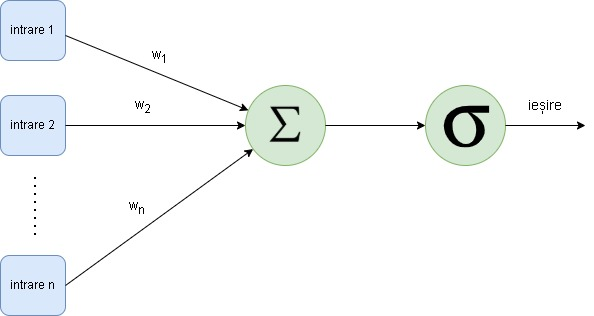
\includegraphics[width=0.6\textwidth]{images/neuron_artificial.jpg} 
    \caption{Reprezentarea schematică a unui neuron artificial: procesarea intrărilor prin ponderare și aplicarea funcției de activare.}
    \label{fig:neuron_artificial}
\end{figure}

Deși aceste rețele au demonstrat performanțe remarcabile, ele prezintă limitări inerente. Utilizarea valorilor numerice continue, conform modelului descris în ecuația \eqref{eq:activare}, forțează sistemul să realizeze calcule intensive în mod constant. Acest aspect conduce la un cost computațional ridicat și la un consum energetic substanțial, care rămâne invariant indiferent de relevanța sau densitatea informației procesate.

\subsection*{Rețele neuronale convoluționale (CNN)}
Rețelele neuronale convoluționale (\textit{Convolutional Neural Networks} -- CNN) reprezintă o categorie specializată de arhitecturi ANN, proiectate explicit pentru procesarea datelor cu structură spațială, cum ar fi imaginile sau secvențele video. Spre deosebire de rețelele complet conectate (\textit{fully connected}), care tratează fiecare pixel ca o intrare independentă, CNN-urile exploatează corelațiile locale dintre pixelii vecini prin intermediul operației de convoluție, reducând drastic numărul de parametri și conferind invarianță la translație.

Operația de convoluție constituie nucleul funcțional al acestor arhitecturi. Un filtru (\textit{kernel}) de dimensiune redusă $k \times k$ este aplicat glisant pe întreaga suprafață a imaginii de intrare, calculând la fiecare poziție $(x,y)$ produsul scalar dintre valorile locale și ponderile filtrului, după cum reiese din ecuația \eqref{eq:convolutie}:
\begin{equation}
	\label{eq:convolutie}
	\text{FeatureMap}(x, y) = \sum_{i=0}^{k-1} \sum_{j=0}^{k-1} I(x+i, y+j) \cdot W(i, j) + b,
\end{equation}
unde $I$ reprezintă imaginea de intrare, $W$ este matricea de ponderi a filtrului, iar $b$ este termenul de \textit{bias}. Rezultatul acestei operații este o \textbf{hartă de trăsături} (\textit{feature map}), care codifică prezența unui anumit tipar vizual (de exemplu, o margine orizontală sau un colț) în diverse regiuni ale imaginii.

O arhitectură CNN tipică este compusă din mai multe tipuri de straturi:
\begin{itemize}[noitemsep]
	\item \textbf{Straturi convoluționale}: Aplică un set de filtre antrenabile, generând hărți de trăsături pentru tipare de complexitate crescândă pe măsura adâncirii rețelei.
	\item \textbf{Straturi de activare}: Introduc neliniaritatea necesară, funcția \textit{ReLU} (\textit{Rectified Linear Unit}), $\sigma(z) = \max(0, z)$, fiind cea mai frecvent utilizată în arhitecturile moderne datorită eficienței sale computaționale și comportamentului stabil la antrenare.
	\item \textbf{Straturi de pooling}: Reduc rezoluția spațială a hărților de trăsături prin agregarea valorilor dintr-o vecinătate locală (ex. \textit{MaxPooling}, \textit{AvgPooling}), conferind robustețe la mici variații de poziție.
	\item \textbf{Straturi complet conectate (Fully Connected)}: Situate la finalul rețelei, realizează maparea vectorului de trăsături extrase către spațiul claselor de ieșire.
\end{itemize}

Antrenarea CNN-urilor se realizează prin algoritmul de \textit{backpropagation}, care propagă eroarea de la stratul de ieșire către straturile anterioare și actualizează ponderile filtrelor prin metoda gradientului descendent. Gradul de expresivitate al acestor rețele crește exponențial cu adâncimea lor, arhitecturi profunde precum ResNet \cite{he2016} sau VGG \cite{simonyan2015very} reușind să extragă trăsături semantice de nivel înalt.

ResNet, utilizat ca extractor de trăsături spațiale, introduce mecanismul \textit{residual connections} (conexiuni reziduale), prin care ieșirea unui bloc de straturi este adunată cu intrarea sa originală în ecuația \eqref{eq:resnet}:
\begin{equation}
	\label{eq:resnet}
	\mathbf{y} = \mathcal{F}(\mathbf{x}, \{W_i\}) + \mathbf{x}.
\end{equation}
Această abordare rezolvă problema dispariției gradientului (\textit{vanishing gradient}) în rețelele adânci, permițând antrenarea eficientă a arhitecturilor cu zeci sau sute de straturi.

\subsection*{Rețele recurente și LSTM}
Rețelele neuronale complet conectate și CNN-urile tratează fiecare intrare ca independentă, ignorând orice dependență temporală sau secvențială. Pentru sarcinile în care ordinea elementelor este esențială -- recunoașterea vorbirii, analiza seriilor de timp sau recunoașterea expresiilor faciale dintr-o secvență video -- această limitare devine critică.

\textbf{Rețelele neuronale recurente} (\textit{Recurrent Neural Networks} -- RNN) adresează această problemă prin introducerea unei bucle de feedback: ieșirea neuronului la pasul temporal $t$ este transmisă ca intrare suplimentară la pasul $t+1$, permițând rețelei să mențină o \textbf{stare ascunsă} (\textit{hidden state}) $\mathbf{h}_t$ care codifică informația acumulată din pașii anteriori. după cum se poate observa în ecuația \eqref{eq:rnn}:
\begin{equation}
	\label{eq:rnn}
	\mathbf{h}_t = \sigma\left(W_h \mathbf{h}_{t-1} + W_x \mathbf{x}_t + b\right).
\end{equation}

Cu toate acestea, RNN-urile clasice suferă de problema dispariției sau explozia gradientului în secvențe lungi: gradientul propagat înapoi prin multe etape temporale tinde fie să se anuleze (împiedicând învățarea dependențelor pe termen lung), fie să crească exponențial (destabilizând antrenamentul).

\textbf{Rețelele LSTM} (\textit{Long Short-Term Memory}), introduse de Hochreiter și Schmidhuber \cite{hochreiter1997}, rezolvă această problemă printr-un mecanism explicit de \textbf{memorie gestionată prin porți} (\textit{gated memory}). Unitatea LSTM menține două stări: starea celulei $\mathbf{c}_t$ (memoria pe termen lung) și starea ascunsă $\mathbf{h}_t$ (memoria pe termen scurt), actualizate conform componentelor descrise în Tabela~\ref{tab:lstm_components}.

\begin{table}[htbp]
	\centering
	\caption{Componentele structurale ale unei unități LSTM și ecuațiile lor matematice.}
	\label{tab:lstm_components}
	\small
	\begin{tabular}{@{} l p{6.5cm} l @{}}
		\hline
		\textbf{Componentă} & \textbf{Rol funcțional} & \textbf{Ecuație de calcul} \\ \hline
		\rule{0pt}{3ex}Poarta de uitare & Decide ce informație din starea anterioară a celulei trebuie eliminată. & $\displaystyle \mathbf{f}_t = \sigma\left(W_f \cdot [\mathbf{h}_{t-1}, \mathbf{x}_t] + b_f\right)$ \\[1.5ex]
		Poarta de intrare & Determină ce proporție din informația nouă va fi transmisă mai departe. & $\displaystyle \mathbf{i}_t = \sigma\left(W_i \cdot [\mathbf{h}_{t-1}, \mathbf{x}_t] + b_i\right)$ \\[1.5ex]
		Starea candidată & Creează un vector cu noile valori potențiale ce pot fi adăugate în starea celulei. & $\displaystyle \tilde{\mathbf{c}}_t = \tanh\left(W_c \cdot [\mathbf{h}_{t-1}, \mathbf{x}_t] + b_c\right)$ \\[1.5ex]
		Poarta de ieșire & Determină ce parte din starea celulei este propagată ca ieșire curentă. & $\displaystyle \mathbf{o}_t = \sigma\left(W_o \cdot [\mathbf{h}_{t-1}, \mathbf{x}_t] + b_o\right)$ \\[1ex] \hline
	\end{tabular}
\end{table}

Actualizarea stărilor se realizează conform relațiilor \eqref{eq:lstm_c_u_update}:
\begin{equation}
	\label{eq:lstm_c_u_update}
	\mathbf{c}_t = \mathbf{f}_t \odot \mathbf{c}_{t-1} + \mathbf{i}_t \odot \tilde{\mathbf{c}}_t, \qquad \mathbf{h}_t = \mathbf{o}_t \odot \tanh(\mathbf{c}_t),
\end{equation}
unde $\odot$ denotă produsul element-cu-element (Hadamard). Prin această arhitectură, LSTM-ul poate reține în mod selectiv informații relevante pe durate arbitrar de lungi, ignorând zgomotul temporal.

Acest mecanism permite modelarea tranzițiilor musculare faciale fine de la faza neutră la apexul emoției. Cu toate acestea, la fel ca toate arhitecturile de învățare profundă din cea de-a doua generație, modelele convoluționale și recurente se confruntă cu două limitări structurale majore: dependența critică de volume masive de date adnotate și costul computațional exorbitant. Pe de o parte, capacitatea de generalizare a acestor rețele este strâns legată de existența unor seturi de date uriașe, curate și etichetate manual, o resursă extrem de costisitoare și dificil de obținut în cazul analizelor de nișă (cum sunt secvențele video dinamice pentru emoții). Pe de altă parte, procesarea continuă și sincronă a matricilor matematice forțează rularea a miliarde de operații în virgulă mobilă (\textit{floating-point operations}) per cadru. Acest aspect generează un consum energetic masiv și o latență incompatibilă cu sistemele încapsulate, menținând o barieră tehnologică rigidă în calea implementării pe dispozitive cu resurse limitate.

\section{Trecerea de la ANN la Spiking Neural Networks (SNN)}

Limitările computaționale și energetice menționate anterior au impus tranziția către o nouă paradigmă: rețelele neuronale cu impulsuri (\textit{Spiking Neural Networks} - SNN). Considerate a treia generație a rețelelor neuronale, SNN-urile se apropie mult mai mult de mecanismele fiziologice ale creierului, înlocuind valorile continue cu impulsuri discrete de joasă energie, numite \textit{spikes} \cite{tavanaei2019deep}.

Spre deosebire de modelele clasice, SNN-urile adoptă o abordare bazată pe evenimente (\textit{event-driven}), caracterizată printr-o activare rară (\textit{sparse activation}), așa cum se poate observa în Figura \ref{fig:ann_vs_snn}. În acest context, neuronii procesează evenimente distribuite temporal, activându-se doar atunci când stimulii recepționați ating un anumit prag critic. Această proprietate elimină necesitatea calculelor redundante în perioadele de inactivitate, optimizând consumul de resurse \cite{falez2019multi}. Mai mult, natura asincronă a acestor rețele facilitează paralelizarea proceselor, oferind avantaje clare de viteză pe hardware neuromorfic dedicat \cite{bing2019supervised}.

\begin{figure}[htbp]
	\centering
	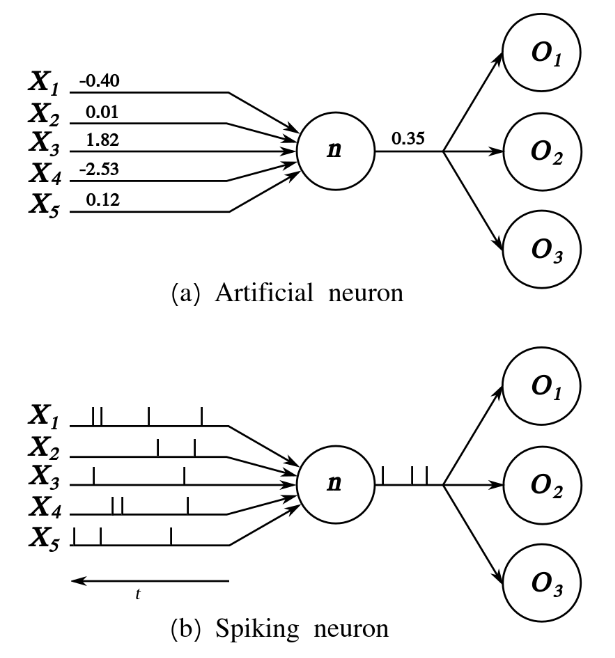
\includegraphics[width=0.45\textwidth]{figures/artificial_vs_spiking_neuron.png}
	\caption{Comparație între un neuron artificial și un neuron cu impulsuri (\textit{spiking neuron}). Sursă: \cite{elassal2024}.}
	\label{fig:ann_vs_snn}
\end{figure}

\section{Modelarea matematică a neuronului cu impulsuri}

Spre deosebire de modelele generațiilor anterioare, rețelele neuronale cu impulsuri (SNN) utilizează ca unitate fundamentală de comunicare fluxuri de impulsuri discrete, cunoscute sub denumirea de \textit{spike trains}. Fiecare impuls reprezintă un potențial de acțiune, o descărcare electrică de scurtă durată care transportă informația prin rețea, imitând fidel procesele electro-chimice din creierul uman.

Mecanismul de funcționare al unui neuron de tip \textit{spiking} este definit prin in\-te\-rac\-ți\-u\-nea dintre potențialul de membrană și un prag de activare (\textit{firing threshold}). Procesul poate fi sintetizat în patru etape critice:

\begin{itemize}
    \item \textbf{Integrarea și acumularea:} Neuronul recepționează semnale de intrare prin sinapse și le cumulează în timp, ceea ce determină o creștere incrementală a potențialului de membrană.
    \item \textbf{Declanșarea (\textit{Firing}):} În momentul în care potențialul acumulat atinge sau depășește valoarea pragului critic stabilit, neuronul generează un impuls de ieșire (\textit{spike}).
    \item \textbf{Resetarea:} Imediat după generarea impulsului, potențialul de membrană revine la o valoare de bază, numită stare de repaus (\textit{resting state}).
    \item \textbf{Perioada refractară:} Urmează un scurt interval de timp în care neuronul devine insensibil la noile impulsuri primite, indiferent de intensitatea acestora, permițând refacerea echilibrului ionic.
\end{itemize}

Evoluția temporală a acestor etape și modul în care potențialul de membrană reacționează la stimulii externi sunt ilustrate în Figura \ref{fig:dinamica_membrana}.

\begin{figure}[htbp]
    \centering
    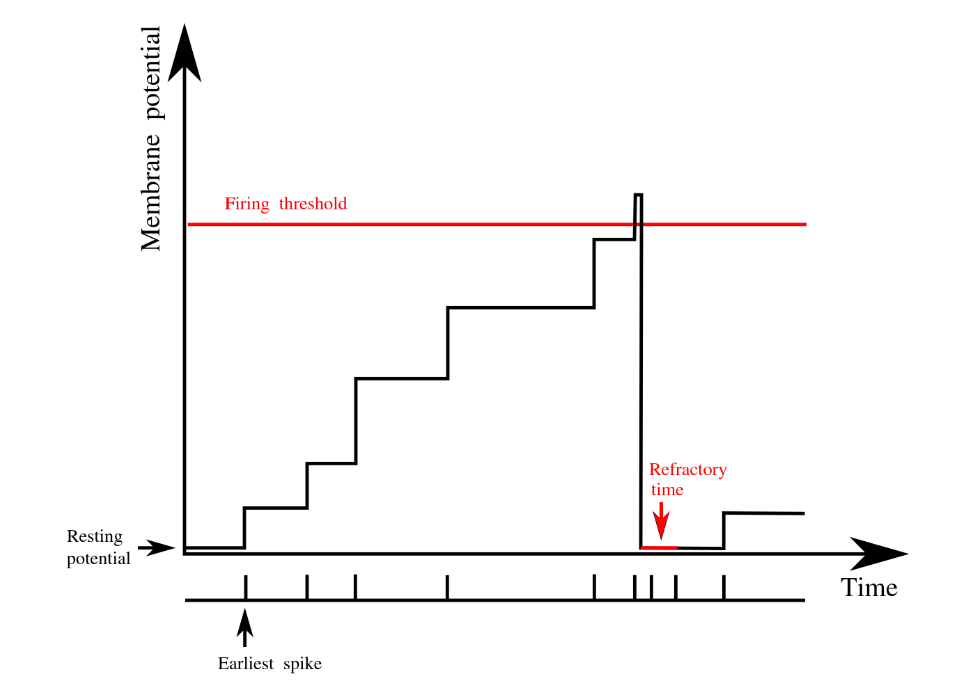
\includegraphics[width=0.75\textwidth]{figures/dinamica_membranei.png}
    \caption{Evoluția potențialului de membrană al unui neuron de tip \textit{spiking} ca răspuns la un tren de impulsuri de intrare. Se observă fazele de acumulare, atingerea pragului critic, generarea impulsului și perioada de resetare. Sursă: \cite{elassal2024}.}
    \label{fig:dinamica_membrana}
\end{figure}

\subsection*{Modele de neuroni: de la biologie la eficiență hardware}
În literatura de specialitate, există o varietate de modele matematice care descriu acest comportament, prezentând un compromis direct între plauzibilitatea biologică și complexitatea computațională \cite{izhikevich2004}.

\begin{enumerate}
    \item \textbf{Modelul Hodgkin-Huxley \cite{hodgkin1952}:} Este unul dintre cele mai detaliate modele biofizice, utilizând un sistem de ecuații diferențiale neliniare pentru a descrie dinamica canalelor ionice (sodiu și potasiu). Deși oferă o acuratețe biologică ridicată, costul computațional necesar pentru simularea acestuia îl face extrem de dificil de implementat în sisteme hardware neuromorfice la scară largă.
    \item \textbf{Modelul Integrate-and-Fire (IF) \cite{burkitt2006}:} Reprezintă varianta cea mai simplificată și eficientă din punct de vedere algoritmic. În ciuda arhitecturii sale elementare, modelul IF s-a dovedit a fi un instrument robust în aplicațiile de învățare vizuală și recunoaștere a formelor, fiind preferat în designul sistemelor de tip \textit{edge AI}.
\end{enumerate}

Modelul IF descrie evoluția potențialului de membrană $V_m(t)$ ca o acumulare liniară a ponderilor sinaptice asociate impulsurilor recepționate. Dinamica sistemului, guvernată de capacitatea membranei $c_m$, este exprimată prin relația \eqref{eq:if_dinamica}:

\begin{equation}
\label{eq:if_dinamica}
c_m V_m(t) = V_r + \sum_{i \in E} w_i f_s(t - t_i),
\end{equation}
unde $V_r$ reprezintă potențialul de repaus al membranei; $E$ constituie setul de impulsuri de intrare; $w_i$ este ponderea sinaptică (greutatea) asociată celui de-al $i$-lea impuls; $t_i$ reprezintă coordonata temporală a recepționării impulsului; iar $f_s$ este funcția nucleu (\textit{spike kernel}), definită conform relației \eqref{eq:spike_kernel}:

\begin{equation}
\label{eq:spike_kernel}
f_s(x) = 
\begin{cases} 
1, & \text{dacă } x \geq 0 \\
0, & \text{în caz contrar}
\end{cases}.
\end{equation}

Regula de actualizare a stării neuronului impune ca atunci când potențialul de membrană depășește pragul $V_{th}$, să aibă loc descărcarea, urmată de resetarea po\-ten\-ți\-a\-lu\-lui, așa cum reiese din relația \eqref{eq:reset_rule}:

\begin{equation}
\label{eq:reset_rule}
V_m(t) \leftarrow V_r, \quad \text{pentru} \quad V_m(t) \geq V_{th}(t).
\end{equation}

Această abordare matematică permite procesarea eficientă a datelor asincrone, fiind ideală pentru sarcini care implică o dinamică temporală complexă, cum este identificarea emoțiilor în secvențe video.

\section{Filtrarea bio-inspirată On/Off}

Înainte ca pixelii bruți ai imaginilor sau cadrelor video să fie transformați în impulsuri temporale, este necesară o etapă de preprocesare capabilă să extragă contrastele spațiale locale și să elimine redundanța informațională. În sistemul vizual biologic, dar și în cazul senzorilor de viziune bazați pe evenimente (DVS), această funcție este îndeplinită de celulele ganglionare retiniene cu structură de tip centru-periferie (\textit{center-surround}). 

Pentru a simula digital acest comportament, se aplică o filtrare liniară bazată pe modelul \textbf{DoG} (\textit{Difference of Gaussians})\cite{rodieck1965quantitative}, care extrage gradienții de contrast prin diferența a două funcții Gaussiene cu deviații standard distincte: una pentru regiunea centrală ($\sigma_{center}$) și una pentru regiunea înconjurătoare ($\sigma_{surround}$). Valoarea rezultată $v$ în urma convoluției imaginii cu filtrul DoG este apoi separată în două canale complet independente, dublând dimensiunea pe adâncime (\textit{depth}) a tensorului de date:

\begin{itemize}[noitemsep]
	\item \textbf{Canalul ON:} Reține exclusiv valorile pozitive ale contrastului, simulând activarea celulelor sensibile la tranziția de la întuneric la lumină (relația \eqref{eq:dog_on}):
	\begin{equation}
		\label{eq:dog_on}
		I_{ON} = \max(0, v).
	\end{equation}
	\item \textbf{Canalul OFF:} Reține magnitudinea valorilor negative (inversate), simulând celulele sensibile la tranziția de la lumină la întuneric (relația \eqref{eq:dog_off}):
	\begin{equation}
		\label{eq:dog_off}
		I_{OFF} = \max(0, -v).
	\end{equation}
\end{itemize}

Pentru a preveni propagarea zgomotului de fond de joasă intensitate și a menține caracterul selectiv (\textit{sparse}) al rețelei, se introduce un parametru de prag critic (\textit{cutoff}). Orice valoare de contrast care nu depășește acest nivel de tăiere este anulată, fiind păstrate doar marginile și formele cu o relevanță semantică ridicată.

Odată realizată separarea structurală în fluxuri ON și OFF, amplitudinile rezultate prezintă scale dinamice, variabile de la un cadru la altul. Deoarece funcția de codificare prin latență (descrisă în secțiunea următoare \ref{sc:codificare}) necesită o intrare strict delimitată în intervalul normat $[0, 1]$, se impune aplicarea modulului \textbf{MaxScaling}. Rolul acestei tehnici este de a normaliza valorile din tensorul filtrat, raportându-le dinamic la valoarea maximă absolută identificată în eșantionul curent, conform relației \eqref{eq:max_scaling}:

\begin{equation}
	\label{eq:max_scaling}
	x_{scaled} = \frac{x}{\max(X)}.
\end{equation}
Această etapă de aliniere garantează că pixelul cu cel mai pronunțat contrast din scenă va fi mapat perfect pe valoarea unitară ($1.0$), devenind ulterior primul impuls generat în timp, facilitând astfel funcționarea corectă a codificării temporale.

\section{Codificarea informației neurale}
\label{sc:codificare}

Întrucât rețelele neuronale cu impulsuri procesează informația sub formă de evenimente discrete, transformarea datelor de intrare (semnale analogice sau valori digitale continue) în trenuri de impulsuri (\textit{spike trains}) reprezintă o etapă fundamentală. În contextul prezentei lucrări, datele de intrare sunt prezentate neuronilor secvențial, eșantion cu eșantion. Fiecare stimul este menținut pentru un interval temporal definit, cunoscut sub numele de perioadă de expunere sau $t_{exposition}$ \cite{falez2019}. 

Deși există numeroase scheme de codificare, acestea pot fi clasificate în două categorii majore, în funcție de modul în care informația este reprezentată în raport cu timpul.

\subsection*{Rate Coding}
Codificarea prin rată corelează intensitatea stimulului de intrare $x \in [0, 1]$ cu frecvența de apariție a impulsurilor. Din punct de vedere computațional, acest proces este modelat printr-un proces stochastic Poisson \cite{gerstner2002spiking}. Probabilitatea ca un neuron $i$ să emită un impuls ($S_i = 1$) într-un interval de timp discret foarte mic $\Delta t$ este proporțională cu valoarea semnalului de intrare, aspect ilustrat în ecuația \eqref{eq:impuls_rate_coding}:

\begin{equation}
\label{eq:impuls_rate_coding}
P(S_i[t] = 1) = x \cdot \Delta t,
\end{equation}
unde $x$ reprezintă intensitatea stimulului (rata de descărcare dorită), $\Delta t$ este pasul de simulare temporală, $S_i[t] \in \{0, 1\}$ este variabila Bernoulli care indică prezența unui impuls la momentul $t$.

Deși este robustă, codificarea prin rată prezintă limitări semnificative în ceea ce privește viteza de procesare. Pentru a obține o reprezentare precisă a valorii codificate, neuronii post-sinaptici trebuie să integreze un număr ridicat de impulsuri pe o durată extinsă \cite{guo2021}. Acest fenomen introduce o latență inerentă în rețea, deoarece decizia este condiționată de acumularea unei statistici suficiente a impulsurilor.

\subsection*{Temporal Coding}
Spre deosebire de codificarea prin rată, metodele temporale utilizează momentul precis al apariției impulsurilor (\textit{timestamps}) pentru a reprezenta informația, oferind o eficiență energetică și temporală superioară.

\subsubsection{Rank Order Coding}
Codificarea prin ordinea rangului \cite{thorpe1998} se bazează pe premisa că ordinea în care neuronii dintr-o populație declanșează impulsuri poartă informația esențială \cite{delorme2001}. Neuronii care primesc stimuli de intensitate ridicată tind să se activeze înaintea celor stimulați slab. O formă simplificată de reprezentare a acestui impact, independentă de modelul de neuron utilizat, este redată de ecuația \eqref{eq:rank_order}:

\begin{equation}
\label{eq:rank_order}
f_{in}(x_i) = r(x_i) \times \frac{1}{n},
\end{equation}
unde $x_i$ este valoarea de intrare, $n$ reprezintă numărul total de conexiuni, iar $r(x_i)$ reprezintă rangul (poziția în ordine descrescătoare) al valorii $x_i$ în setul de intrări.

\subsubsection{Latency Coding}
Codificarea prin latență \cite{gollisch2008} reprezintă intensitatea stimulului prin intervalul de timp scurs până la primul impuls. Un stimul puternic va genera un răspuns rapid (latență mică), în timp ce un stimul slab va întârzia activarea neuronului. Relația de inversă proporționalitate între intensitatea $x$ și momentul declanșării este formalizată prin ecuația \eqref{eq:latency}:

\begin{equation}
\label{eq:latency}
f_{in}(x) = (1.0 - x) \times t_{exposition}.
\end{equation}

Această abordare este deosebit de eficientă pentru procesarea video, deoarece permite rețelei să reacționeze extrem de rapid la schimbările semnificative din câmpul vizual, procesând prioritar cele mai relevante informații.

\section{Mecanisme de învățare și plasticitate sinaptică}

Capacitatea de procesare a informației în cadrul rețelelor SNN rezidă în conexiunile sinaptice dintre neuroni. \textbf{Plasticitatea sinaptică} reprezintă proprietatea fundamentală a acestor conexiuni de a-și modifica intensitatea (ponderea sinaptică) în funcție de tiparele activității neuronale și de regulile de învățare aplicate. Din punct de vedere funcțional, ponderile sinaptice modulează probabilitatea de declanșare a neuronului post-sinaptic: o pondere ridicată amplifică contribuția unui impuls recepționat, în timp ce o pondere scăzută atenuează impactul acestuia asupra po\-ten\-ți\-a\-lu\-lui de membrană.

Antrenarea acestor rețele presupune ajustarea sistematică a ponderilor și a pragurilor de activare pentru a permite sistemului să identifice trăsături relevante în datele de intrare. În literatura de specialitate, metodele de antrenare a SNN-urilor pot fi clasificate în trei paradigme majore.

\subsection*{Conversia ANN în SNN}
Această abordare presupune antrenarea prealabilă a unei rețele neuronale artificiale (ANN) convenționale, utilizând algoritmi standard precum \textit{Backpropagation}, urmată de transferul și adaptarea ponderilor învățate către o arhitectură SNN echivalentă \cite{kugele2020}. 

Procesul de conversie urmărește conservarea funcționalității și a performanței rețelei originale prin scalarea ponderilor și ajustarea acestora la intervalul dinamic specific modelului de neuron cu impulsuri ales. Deși această metodă oferă rezultate competitive și permite utilizarea infrastructurii software existente pentru \textit{Deep Learning}, ea prezintă limitări critice:
\begin{itemize}
    \item Necesită resurse computaționale ridicate pentru etapa inițială de antrenare a ANN-ului.
    \item Implică procese post-conversie complexe, precum normalizarea ponderilor și echilibrarea pragurilor (\textit{threshold balancing}).
    \item Nu exploatează pe deplin avantajele temporale native ale SNN-urilor în timpul procesului de învățare.
\end{itemize}

\subsection*{Spiking back-propagation}
O altă metodă supervizată constă în adaptarea directă a algoritmului \textit{Backpropagation} pentru domeniul impulsurilor \cite{grum23}. Această tehnică optimizează ponderile prin calcularea unei funcții de cost bazată pe eroarea dintre ieșirea dorită și cea prezisă, eroarea fiind ulterior propagată de la stratul de ieșire către straturile anterioare.

Principala provocare a acestei metode rezidă în faptul că funcția de activare a unui neuron \textit{spiking} (funcția Heaviside) este discontinuă și, prin urmare, nederivabilă \cite{lee2016}. Acest aspect împiedică calculul direct al gradientului necesar optimizării. Pentru a depăși acest obstacol, cercetările recente propun:
\begin{itemize}
    \item Utilizarea unor \textbf{gradienți surogat} (\textit{surrogate gradients}) care aproximează derivata impulsului în timpul etapei de \textit{backward pass} \cite{tavanaei2019deep}.
    \item Tratarea potențialului de membrană ca pe un semnal continuu și derivabil \cite{lee2016}.
\end{itemize}

Deși metoda este eficientă pentru obținerea unei precizii ridicate, ea rămâne costisitoare din punct de vedere computațional și necesită volume mari de date etichetate, ceea ce limitează aplicabilitatea sa în sistemele de tip \textit{on-chip learning} cu resurse reduse \cite{lee2018_frontiers}.

\subsection*{Învățarea de tip Hebbian}

Plasticitatea de tip Hebbian constituie un principiu fundamental în neuroștiințe, stipulând că intensitatea unei sinapse între doi neuroni este determinată de corelația activităților acestora. Conform celebrului postulat al lui Donald Hebb: „neuronii care se activează împreună, se conectează împreună” (\textit{neurons that fire together, wire together}) \cite{hebb2002}. În domeniul SNN, învățarea Hebbiană este utilizată pe scară largă pentru antrenarea rețelelor în regim supervizat \cite{lan2022pcsnn}, nesupervizat \cite{kheradpisheh2018stdp} sau auto-supervizat \cite{halvagal2023combination}.

Mecanismul de bază presupune modificarea greutății sinaptice în funcție de co\-re\-la\-ți\-a dintre activitatea pre-sinaptică (intrarea) și cea post-sinaptică (ieșirea). Deși există mai multe reguli de plasticitate, precum \textit{Spike-Driven Synaptic Plasticity} (SDSP), majoritatea aplicațiilor contemporane se bazează pe \textbf{Spike Timing-Dependent Plasticity (STDP)}, datorită robusteții sale în procesarea semnalelor temporale.

STDP este o regulă de învățare cu înaltă plauzibilitate biologică \cite{song2000competitive} ce ajustează ponderile sinaptice pe baza diferenței temporale relative dintre impulsurile pre-sinaptice și cele post-sinaptice. Această metodă este esențială pentru implementările pe hardware neuromorfic cu consum redus, fiind capabilă să extragă trăsături complexe fără necesitatea unei supervizări externe.

Principiul de funcționare al STDP se bazează pe două fenomene opuse, așa cum este observat experimental în mod sistematic în lucrarea lui Bi și Poo \cite{bi1998synaptic}:
\begin{itemize}
    \item \textbf{Potențarea pe termen lung (Long-Term Potentiation - LTP):} Dacă impulsul pre-sinaptic are loc cu puțin timp înaintea impulsului post-sinaptic, sinapsa este întărită. Acest lucru sugerează că intrarea a contribuit direct la activarea neuronului.
    \item \textbf{Depresia pe termen lung (Long-Term Depression - LTD):} Dacă impulsul post-sinaptic are loc înaintea celui pre-sinaptic, sinapsa este slăbită. Aceasta indică faptul că semnalul de intrare nu a avut un rol cauzal în declanșarea impulsului de ieșire.
\end{itemize}

Această dinamică permite rețelei să prioritizeze conexiunile care transportă in\-for\-ma\-ți\-e relevantă pentru modelul identificat, ignorând în același timp zgomotul sau semnalele necorelate temporal.

În funcție de complexitatea dorită și de constrângerile hardware, STDP poate fi implementată prin mai multe modele matematice:

\paragraph{1. STDP Biologic:}
Este forma de bază care utilizează o descreștere exponențială a actualizării ponderii în funcție de distanța temporală dintre impulsuri \cite{bi1998synaptic}. Formalizarea matematică este dată de ecuația \eqref{eq:stdp_biologic}:

\begin{equation}
\label{eq:stdp_biologic}
\Delta w = 
\begin{cases} 
\eta_w e^{-\frac{t_{post} - t_{pre}}{\tau_{STDP}}}, & \text{dacă } t_{pre} \leq t_{post} \\
-\eta_w e^{-\frac{t_{pre} - t_{post}}{\tau_{STDP}}}, & \text{în caz contrar}
\end{cases},
\end{equation}
unde $\eta_w$ reprezintă rata de învățare, iar $\tau_{STDP}$ este constanta de timp ce definește fereastra de învățare.

\paragraph{2. STDP Aditiv (Add-STDP):}
O variantă simplificată unde modificarea ponderii depinde doar de semnul diferenței temporale, nu și de magnitudine. Deoarece poate conduce la instabilitate, aceasta necesită limite stricte de control (\textit{hard boundaries}), rezultând adesea în ponderi binare (0 sau 1) \cite{song2000competitive}, așa cum este ilustrat în ecuația \eqref{eq:add_stdp}:

\begin{equation}
\label{eq:add_stdp}
\Delta w = 
\begin{cases} 
\eta_{w+}, & \text{dacă } \delta t \leq 0 \\
-\eta_{w-}, & \text{în caz contrar}
\end{cases}.
\end{equation}

\paragraph{3. STDP Multiplicativ (Mult-STDP):}
Această variantă introduce dependența de valoarea curentă a ponderii, prevenind saturarea și oferind o distribuție mai fină a greutăților sinaptice, comparativ cu modelul aditiv \cite{rossum2000}. Actualizarea surprinsă în ecuația \eqref{eq:mult_stdp} este reglată astfel încât ponderile mici să poată crește mai rapid, în timp ce ponderile mari sunt limitate superior:

\begin{equation}
\label{eq:mult_stdp}
\Delta w = 
\begin{cases} 
\eta_{w+} e^{-\beta \frac{w - w_{min}}{w_{max} - w_{min}}}, & \text{dacă } \delta t \leq 0 \\
-\eta_{w-} e^{-\beta \frac{w_{max} - w}{w_{max} - w_{min}}}, & \text{în caz contrar}
\end{cases}.
\end{equation}

\subsection*{Inhibiția}

Inhibiția reprezintă procesul de diminuare sau suprimare a activității neuronale, fiind un mecanism fundamental pentru reglarea dinamicii corticale \cite{silberberg2007disynaptic}. Într-o rețea neuronală cu impulsuri (SNN), inhibiția joacă un rol vital în menținerea echilibrului dintre mecanismele excitatorii și cele inhibitorii, permițând un control precis asupra fluxului de informație și a momentelor de declanșare a impulsurilor \cite{zhao2022backeisnn}.

Cea mai utilizată metodă de inhibiție în faza de antrenare este mecanismul \textit{Winner-Take-All} (WTA) \cite{querlioz2011simulation, chen2017mechanisms}. Conform acestei reguli, primul neuron dintr-un strat care generează un impuls este declarat „câștigător” și transmite imediat un semnal inhibitor către ceilalți neuroni din același strat pentru a le bloca activitatea. Această strategie este deosebit de eficientă în învățarea nesupervizată bazată pe STDP, deoarece introduce o competiție între neuroni \cite{ferre2018unsupervised}. Prin împiedicarea mai multor neuroni să răspundă simultan la același stimul, rețeaua este forțată să învețe trăsături distincte și mai puțin corelate, optimizând astfel capacitatea de reprezentare a sistemului.

\subsection*{Homeostazia}

Deși mecanismul \textit{Winner-Take-All} (WTA) este esențial pentru diversificarea procesului de învățare, acesta poate introduce un dezechilibru în care un număr restrâns de neuroni devin dominanți. Acești neuroni „câștigători” tind să se declanșeze repetat, monopolizând procesul de adaptare a ponderilor, în timp ce restul unităților rămân inactive. Pentru a evita această saturație și a menține stabilitatea sistemului, este necesară implementarea unor mecanisme de homeostazie prin adaptarea pragului de declanșare (\textit{threshold adaptation}).

Cu scopul de a regla competiția dintre neuroni și de a asigura o activare echilibrată în straturile unde aceștia concurează, se utilizează două metode complementare de adaptare a pragului. Prima și cea mai importantă este \textbf{Leaky Adaptive Threshold (LAT)} \cite{diehl2015}, utilizată pentru a asigura o competiție echitabilă între neuroni. Cea de-a doua este metoda \textbf{adaptării pragului bazată pe un timp țintă} (\textit{target timestamp}) \cite{falez2019multi}, utilizată în conjuncție cu LAT în modelele de tip CSNN de ultimă generație \cite{falez2019}. Aceasta din urmă forțează neuronii să tindă spre un moment de declanșare predefinit $\hat{t}$, permițând modelului să se specializeze pe anumite tipare temporale, contribuind în același timp la homeostazia rețelei.

Pragurile tuturor neuronilor dintr-un strat (atât pentru cel câștigător, cât și pentru cei care au primit semnal de inhibiție) sunt actualizate la fiecare declanșare a unui impuls sau la recepția unui semnal inhibitor. Din punct de vedere matematic, modificarea pragului se bazează pe două componente, $\Delta_{th}^1$ și $\Delta_{th}^2$, după cum reiese din ecuația \eqref{eq:target_timestamp}:

\begin{equation}
\label{eq:target_timestamp}
\Delta_{th}^1 = -\eta_{th}(t - \hat{t}),
\end{equation}
unde $t$ este momentul declanșării impulsului, $\hat{t}$ este timpul țintă dorit, iar $\eta_{th}$ este rata de învățare a pragului. 
Componenta LAT este definită în ecuația \eqref{eq:lat_update}:

\begin{equation}
\label{eq:lat_update}
\Delta_{th}^2 = 
\begin{cases} 
\eta_{th}, & \text{dacă } t_i = \min\{t_0, \dots, t_N\} \\
-\frac{\eta_{th}}{ld(n)}, & \text{în caz contrar}
\end{cases},
\end{equation}
unde $t_i$ reprezintă timpul de declanșare al neuronului $i$, $\min\{t_0, \dots, t_N\}$ corespunde neuronului care a generat primul impuls (câștigătorul), iar $ld(n)$ reprezintă numărul de neuroni aflați în competiție în stratul respectiv. În final, actualizarea potențialului pragului de membrană $V_{th}$ se realizează conform ecuației \eqref{eq:vth_final}:

\begin{equation}
\label{eq:vth_final}
V_{th}(t) = \max(th_{min}, V_{th}(t-1) + \Delta_{th}^1 + \Delta_{th}^2),
\end{equation}
unde $th_{min}$ reprezintă valoarea minimă admisă a pragului \cite{falez2019}, asigurând astfel că sensibilitatea neuronului nu crește peste o limită care ar putea genera activitate spontană cauzată de zgomot. Această abordare combinată asigură faptul că latența impulsurilor converge către valoarea țintă, menținând în același timp un echilibru între activitatea tuturor celor $N$ neuroni din strat.

\section{Arhitecturi Convolutional Spiking Neural Networks (CSNN)}

Arhitecturile Convolutional Spiking Neural Networks (CSNN) combină capacitatea de extragere a trăsăturilor spațiale cu eficiența energetică a neuronilor de tip spiking. Este important de subliniat că dinamica antrenării variază esențial în funcție de paradigma de învățare aleasă. În timp ce abordările supervizate pot actualiza și propaga ponderile simultan într-un singur flux end-to-end prin intermediul gradienților surogat (\textit{surrogate gradients}), rețelele bazate pe învățare bio-inspirată nesupervizată impun o decuplare structurală. Astfel, pentru modelele CSNN nesupervizate (precum arhitectura investigată în prezenta lucrare), implementarea unui strat de con\-vo\-lu\-ți\-e presupune o metodologie ierarhică, structurată în două etape distincte:

1. \textbf{Etapa de învățare (Learning Phase):} Această fază se bazează în mod critic pe un proces de eșantionare locală. Un fragment de interes (\textit{patch}) este extras din fluxul de date de intrare, iar nucleele de convoluție (\textit{kernels}) concurente rulează un mecanism de competiție locală de tip \textit{auto-inhibiție} direct pe suprafața acestui sub-spațiu. Fiecare nucleu este asociat unui neuron specific, iar scopul competiției este adaptarea ponderilor sinaptice $W$ prin regula STDP, forțând filtrul învingător să se specializeze exclusiv pe tiparul vizual sau dinamic dominant din \textit{patch}-ul selectat. Acest mecanism local de eșantionare constituie pilonul central al prezentei lucrări și va fi tratat pe larg, cu toate implicațiile sale arhitecturale, în secțiunea~\ref{sc:sampling}.

2. \textbf{Etapa de testare/inferență (Inference Phase):} Odată ce ponderile au fost învățate, acestea sunt „înghețate” și replicate pe întreaga suprafață a intrării. În această etapă, se asociază neuroni virtuali pentru fiecare element din hărțile de trăsături rezultate. Esențial este faptul că toate unitățile dintr-o hartă de trăsături partajează același nucleu învățat anterior, asigurând invarianța la translație și același prag de declanșare global. Pe parcursul inferenței, selecția caracteristicilor este guvernată de mecanismul strict de auto-inhibiție temporală. Acesta presupune că, pentru a preveni activările redundante în cadrul aceluiași eșantion, orice neuron virtual care a emis un spike este marcat ca inhibat în acea locație din feature map, fiindu-i interzisă o nouă declanșare până la procesarea următorului eșantion.

\subsection*{Convoluția în domeniul impulsurilor (2D-CSNN)}

Generarea hărților de trăsături în etapa de inferență se realizează prin aplicarea glisantă a filtrului (Figura ~\ref{fig:conv2d}), unde dinamica potențialului de membrană pentru un neuron de tip \textit{Integrate-and-Fire} (IF) de la coordonatele $(x, y)$ este calculată conform ecuației \eqref{eq:conv_spiking}:

\begin{equation}
\label{eq:conv_spiking}
V_{m_{x,y,k}}(t) = \sum_{i \in E} W_{n(x_i), j(y_i), k_i, k} \cdot f_s(t - t_i),
\end{equation}
unde $f_s(t - t_i)$ guvernează evoluția temporală a răspunsului postsinaptic în funcție de timpul scurs de la apariția impulsului, $n(x_i)$ și $j(y_i)$ mapează coordonatele spațiale ale impulsului de intrare în fereastra locală a nucleului (kernelului) 2D, iar $k_i$ și $k$ reprezintă canalul de origine (intrare), respectiv canalul hărții de trăsături țintă (ieșire).

\begin{figure}[htbp]
    \centering
    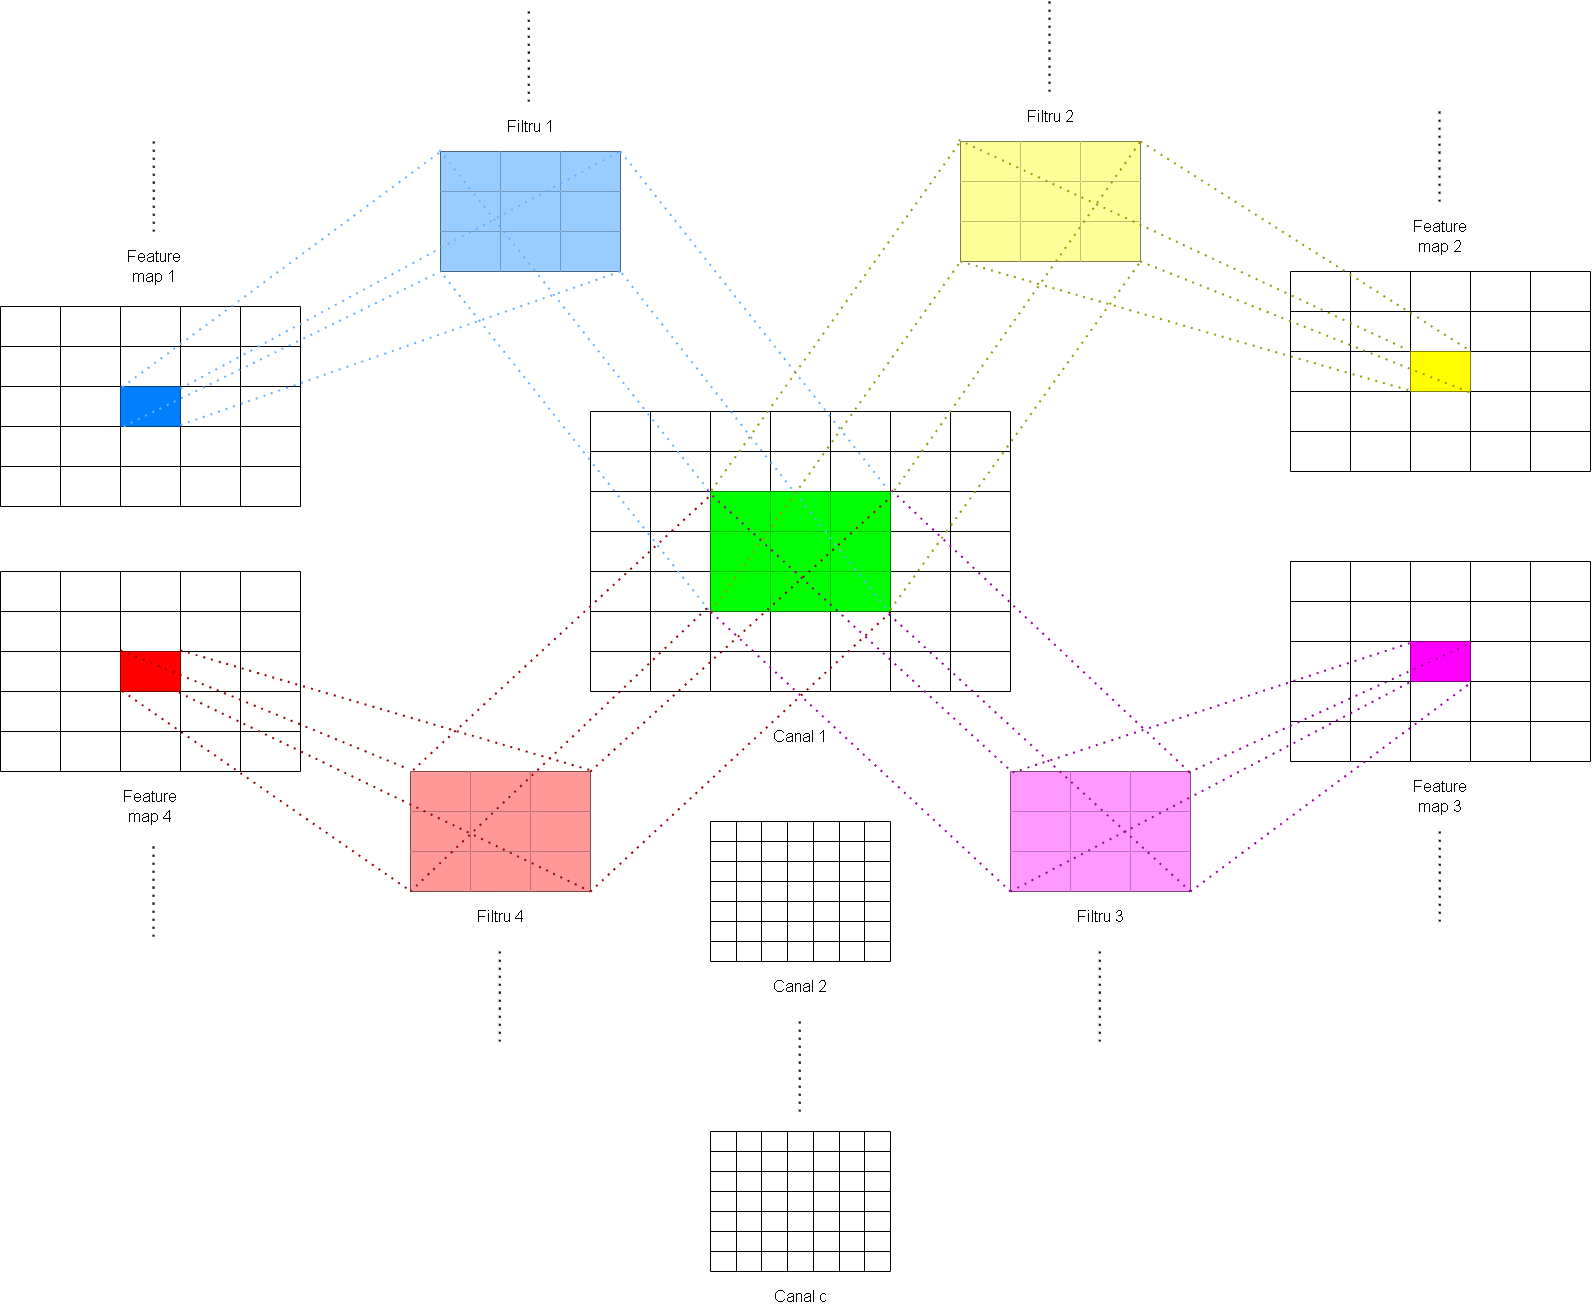
\includegraphics[width=0.7\textwidth]{figures/2d-csnn.png}
    \caption{Reprezentarea procesului de convoluție 2D.}
    \label{fig:conv2d}
\end{figure}

\subsection*{3D-CSNN pentru procesare video}

Extensia către 3D-CSNN urmează aceeași logică bimodală (învățare vs. testare), dar extinde domeniul de aplicare în dimensiunea temporală. Această arhitectură permite extragerea directă a trăsăturilor spatio-temporale, eliminând necesitatea unor algoritmi externi de calcul al fluxului optic \cite{horn1981determining}.

În etapa de inferență 3D, nucleul glisant integrează informația dintr-un volum de intrare (lățime, înălțime și adâncime temporală), procesul fiind ilustrat în Figura”\ref{fig:conv3d}). Toți neuronii dintr-un volum de ieșire $k$ utilizează același set de ponderi 3D învățate, calculând potențialul de membrană la momentul $t$ conform formulei \eqref{eq:conv3d_spiking}:

\begin{equation}
\label{eq:conv3d_spiking}
V_{m_{x,y,z,k}}(t) = \sum_{i \in E} W_{n(x_i), j(y_i), h(z_i), k_i, k} \cdot f_s(t - t_i),
\end{equation}
unde $h(z_i)$ mapează coordonata temporală a impulsului în fereastra nucleului 3D. Acest mecanism permite neuronilor să devină selectivi la schimbări dinamice, simulând comportamentul neuronilor din cortexul vizual primar care răspund la direcții specifice de mișcare în câmpul receptiv.

\begin{figure}[htbp]
    \centering
    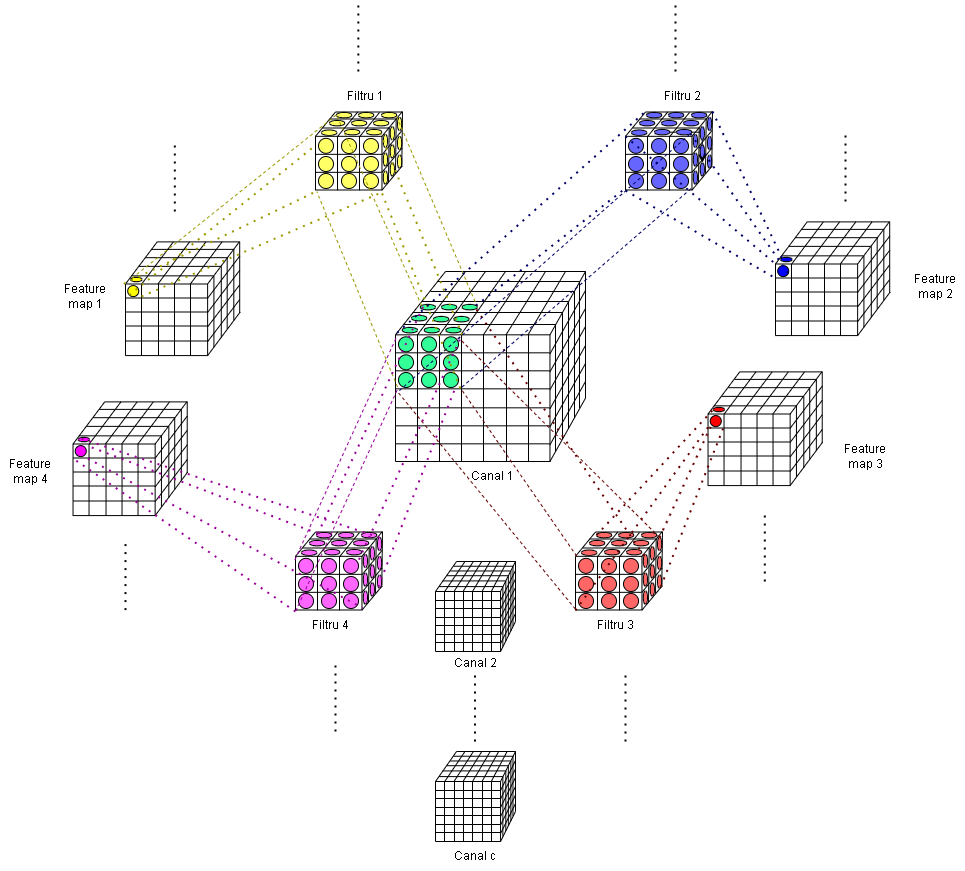
\includegraphics[width=0.75\textwidth]{figures/3d-csnn.png}
    \caption{Operația de convoluție 3D. Aceasta procesează „cuburi” de evenimente, unde aceeași matrice de ponderi $W$ este utilizată pentru a scana întregul flux video.}
    \label{fig:conv3d}
\end{figure}



\section{Metode de eșantionare spațio-temporală a datelor de intrare}
\label{sc:sampling}

În cadrul arhitecturilor de tip Convolutional Spiking Neural Networks (CSNN) aplicate asupra secvențelor video, procesul de eșantionare (\textit{sampling}) joacă un rol critic în eficiența procesării informației vizuale din cadrul etapei de învățare. Spre deosebire de rețelele convoluționale clasice, unde întreaga secvență video este procesată uniform, simulatoarele de SNN pot utiliza strategii de eșantionare pentru a selecta volume locale (\textit{spatio-temporal patches}) care urmează să fie convertite în trenuri de impulsuri (\textit{spikes}).

Această abordare este inspirată din mecanismele biologice de atenție vizuală, permițând modelului să se concentreze pe regiunile cele mai informative ale scenei și pe modificările acestora în timp, reducând astfel costul computațional și influența zgomotului de fundal. În cadrul acestui simulator, au fost implementate patru strategii principale de eșantionare spațio-temporală (3D), în care selecția datelor are loc simultan pe axele spațiale $(x, y)$ și temporală $(t)$. Rezultatul procesului de eșantionare este un volum de date definit de coordonatele $(x, y, t)$, unde $(x, y)$ reprezintă poziția spațială a ferestrei, iar $t$ momentul de start al secvenței temporale analizate.

\subsection*{Eșantionarea aleatorie}

Metoda de eșantionare aleatorie reprezintă abordarea de bază, în care locația volumului de filtrare este determinată în mod stohastic pe întreaga suprafață spațio-temporală a secvenței de intrare. Coordonatele spațiale ale colțului stânga-sus al ferestrei, $(x, y)$, precum și momentul temporal de start $t$, sunt extrase din distribuții uniforme, respectând constrângerile dimensionale ale videoclipului, după cum reiese din relațiile \eqref{eq:distributii_random}:

\begin{equation}
	\label{eq:distributii_random}
	x \sim \mathcal{U}(0, W - w_f), \quad
	y \sim \mathcal{U}(0, H - h_f), \quad
	t \sim \mathcal{U}(0, T - t_f),
\end{equation}
unde $W$ și $H$ reprezintă lățimea și înălțimea cadrului video, $T$ durata totală a secvenței, iar $w_f$, $h_f$ și $t_f$ dimensiunile filtrului pe axele spațiale și temporală.

\subsection*{Strategii faciale bazate pe bounding box}

Pentru a restrânge spațiul de căutare la regiunea facială (\textit{Region of Interest -- ROI}), se utilizează casete de delimitare (\textit{bounding boxes}) detectate în prealabil. Această abordare reduce probabilitatea eșantionării zonelor irelevante și garantează că volumele extrase conțin informație facială relevantă pentru clasificarea emoțiilor. Pentru fiecare fereastră temporală selectată, se calculează o regiune de reuniune (\textit{Union Bounding Box}) care include toate casetele de delimitare asociate cadrelor din intervalul temporal: [$t$, $t+t_f$]. Prin această strategie se garantează faptul că, indiferent de mișcarea capului în cadrul secvenței analizate, volumul extras va conține în permanență regiunea facială a subiectului.

\subsection*{Eșantionarea bazată pe landmark-uri faciale}

Această metodă bazată pe puncte de reper faciale (\textit{facial landmarks}) se fundamentează pe ipoteza că emoțiile feței sunt reprezentate predominant prin variațiile micro-expresiilor localizate în jurul ochilor, sprâncenelor, nasului și gurii. În loc să selecteze volume în mod arbitrar, metoda prioritizează regiunile cu densitate in\-for\-ma\-țio\-na\-lă ridicată, imitând mecanismele biologice ale sistemului vizual uman.

Selecția punctelor de reper urmează schema standard de adnotare cu 68 de land\-mark-uri propusă în setul de date 300-W \cite{sagonas2013300w}, utilizată extensiv în biblioteci precum Dlib sau MediaPipe. Reprezentarea acestor puncte de reper faciale este ilustrată în Figura~\ref{fig:landmarks_68}, iar distribuția lor este prezentată în Tabela~\ref{tab:landmarks}.

\begin{figure}[htbp]
	\centering
	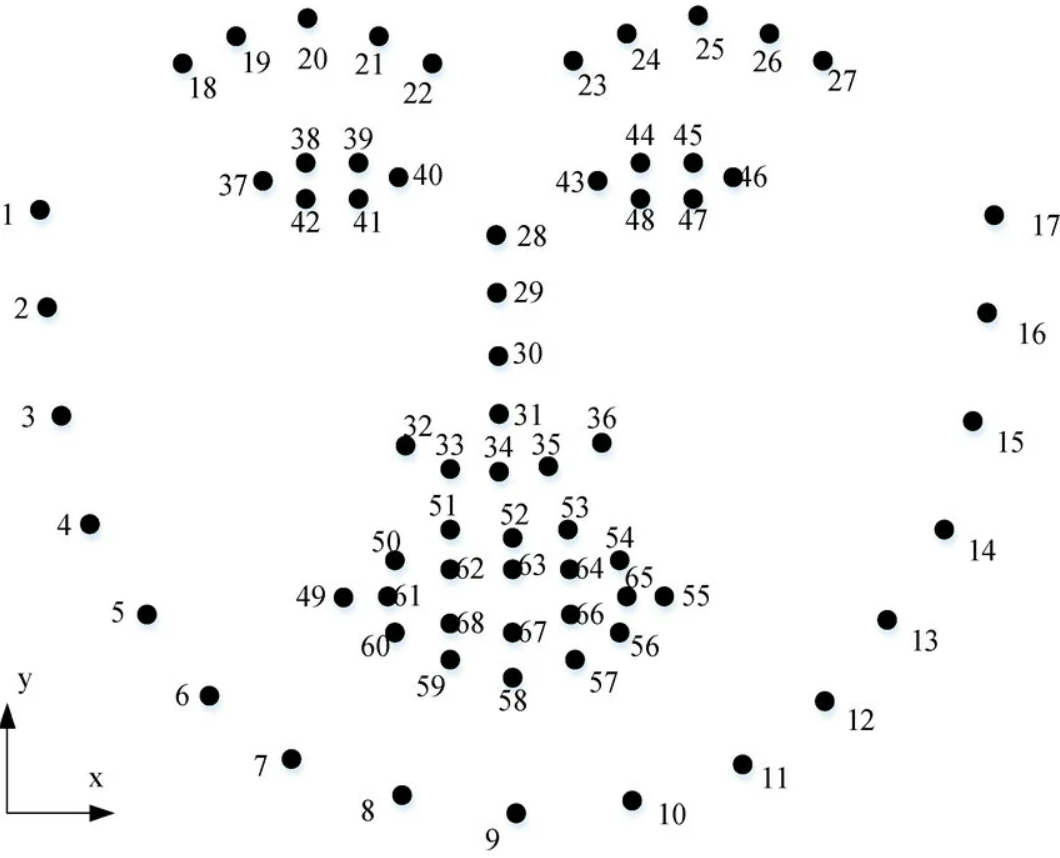
\includegraphics[width=0.7\textwidth]{figures/landmarks_68.png}
	\caption{Reprezentarea celor 68 de puncte de reper faciale (\textit{landmarks}) conform standardului 300-W \cite{li2019}.}
	\label{fig:landmarks_68}
\end{figure}

\begin{table}[h]
	\centering
	\caption{Distribuția punctelor de reper faciale în formatul standard de 68 de puncte.}
	\label{tab:landmarks}
	\begin{tabular}{|l|l|}
		\hline
		\textbf{Regiune Facială} & \textbf{Indici (0-indexed)} \\ \hline
		Contur Mandibulă         & 0 -- 16                     \\ \hline
		Sprânceana Dreaptă       & 17 -- 21                    \\ \hline
		Sprânceana Stângă        & 22 -- 26                    \\ \hline
		Puntea Nazală            & 27 -- 30                    \\ \hline
		Baza Nasului             & 31 -- 35                    \\ \hline
		Ochiul Drept             & 36 -- 41                    \\ \hline
		Ochiul Stâng             & 42 -- 47                    \\ \hline
		Contur Exterior Gură     & 48 -- 59                    \\ \hline
		Contur Interior Gură     & 60 -- 67                    \\ \hline
	\end{tabular}
\end{table}

În cadrul implementării, intervalul de indici $[17, 67]$ este selectat pentru a exclude conturul mandibulei (\textit{jawline}), considerat mai puțin relevant pentru exprimarea emoțiilor, și pentru a maximiza probabilitatea eșantionării trăsăturilor faciale cu valoare semantică ridicată.

Logica algoritmică a metodei presupune parcurgerea mai multor etape. Procedura de eșantionare începe prin selectarea uniformă a unui moment de start $t$ din secvența de intrare. Un punct de reper este apoi ales aleatoriu din subsetul expresiv $[17, 67]$, iar fereastra de extracție spațială de dimensiunea $w_f \times h_f$ este centrată pe coordonatele reperului selectat. Pentru a îmbunătăți robustețea structurală și a reduce \textit{overfittingul}, se introduce o mică perturbație uniformă aleatorie a coordonatelor (\textit{jitter}) în intervalul $[-2, 2]$ pixeli. În cele din urmă, se aplică funcții de \textit{clamping } pentru a se asigura că regiunea extrasă rămâne în limitele video valide.

Această strategie permite rețelei CSNN să urmărească evoluția temporală a unei trăsături faciale specifice (de exemplu curbura gurii în timpul unui zâmbet sau modificările subtile din jurul ochilor asociate expresiilor emoționale) fără necesitatea procesării întregului cadru video.

\subsection*{Eșantionarea bazată pe filtrul ON/OFF}

A patra strategie implementată introduce un mecanism de eșantionare ghidată de relevanță (\textit{saliency-guided sampling}), conceput pentru a prioritiza regiunile spațio-temporale cu activitate neuronală ridicată după aplicarea filtrării de tip DoG și a codificării în impulsuri (\textit{spike encoding}).

Motivația acestei metode pornește de la observația că, în cadrul sistemelor vizuale biologice, atenția este orientată în mod natural către regiunile cu contrast local puternic și variații temporale semnificative. În mod similar, după aplicarea filtrelor ON/OFF de tip DoG, pixelii care prezintă tranziții de intensitate relevante sau modificări expresive subtile generează activitate neuronală mai intensă, reprezentând candidați superiori pentru procesarea ulterioară.

Spre deosebire de strategiile precedente, unde selecția este uniformă sau ghidată geometric, această metodă realizează eșantionarea utilizând o distribuție probabilistică dependentă de relevanța locală a datelor de intrare.

În mod opțional, procesul poate fi restrâns la regiunea facială prin utilizarea casetelor de delimitare (\textit{bounding boxes}), reducând influența fundalului și limitând selecția la zona de interes facială.

Procesul de selecție este realizat în două etape succesive: temporală și spațială.

\subsubsection{Selecția temporală bazată pe relevență}

În prima etapă este determinat momentul temporal $t$ în jurul căruia va fi extras volumul spațio-temporal. Pentru fiecare cadru temporal se calculează un scor global de relevență, obținut prin agregarea activității tuturor pixelilor din regiunea de interes, conform ecuației \eqref{eq:temp_saliency}:

\begin{equation}
	\label{eq:temp_saliency}
	S_t = \sum_{x,y \in ROI} s(x,y,t),
\end{equation}
unde $s(x,y,t)$ reprezintă scorul de relevență asociat pixelului $(x,y)$ la momentul $t$.

În cazul utilizării codificării prin latență (\textit{latency coding}), activitatea neuronală este invers proporțională cu timpul de activare al spike-ului. Astfel, pixelii care generează impulsuri timpurii primesc ponderi mai mari, după cum se poate observa în ecuația \eqref{eq:impuls_latency}.

\begin{equation}
	\label{eq:impuls_latency}
	s(x,y,t)=\max(0,1-v(x,y,t)),
\end{equation}
unde $v(x,y,t)$ reprezintă latența asociată spike-ului. În absența codificării prin latență, scorul este determinat direct din amplitudinea activării.

După calcularea scorurilor temporale, cadrul de interes este selectat utilizând o metodă de tip \textit{roulette wheel selection} (selecție proporțională cu probabilitatea), în care probabilitatea de alegere a unui moment temporal este dată de ecuația \eqref{eq:prob_temp}.

\begin{equation}
	\label{eq:prob_temp}
	P(t)=\frac{S_t}{\sum_k S_k}.
\end{equation}

Prin această formulare, cadrele care conțin activitate neuronală intensă (asociată de regulă mișcărilor faciale subtile sau schimbărilor expresive) au o probabilitate mai mare de a fi selectate.

\subsubsection{Selecția spațială bazată pe relevență}

După determinarea cadrului temporal, procesul continuă prin selecția coordonatelor spațiale $(x,y)$ utilizând aceeași logică probabilistică.

Pentru cadrul selectat, fiecărui pixel din regiunea de interes îi este asociat un scor de relevență, iar probabilitatea de selecție urmează ecuația \eqref{eq:probab_sp}.

\begin{equation}
	\label{eq:probab_sp}
	P(x,y \mid t)=
	\frac{s(x,y,t)}
	{\sum_{i,j \in ROI} s(i,j,t)}.
\end{equation}

Astfel, pixelii care prezintă activitate neuronală ridicată după filtrarea ON/OFF (de exemplu marginile gurii în timpul unui zâmbet sau zona ochilor în expresii de surpriză) au șanse semnificativ mai mari de a deveni centrul volumului eșantionat.

După alegerea punctului central, fereastra spațială de dimensiune $w_f \times h_f$ este poziționată astfel încât pixelul selectat să fie centrat în interiorul acesteia. Ulterior, se aplică o operație de \textit{clamping} pentru a garanta că volumul rezultat rămâne în limitele valide ale secvenței video.

\subsubsection{Mecanism de explorare}

Pentru a evita supra-specializarea modelului asupra acelorași regiuni relevente și pentru a menține diversitatea eșantioanelor, metoda introduce un mecanism explicit de explorare (\textit{exploration factor}).

Cu o probabilitate controlată de parametrul $\alpha \in [0,1]$, denumit factor de explorare (\textit{random mix}), selecția ghidată de relevență este ignorată, iar volumul este extras prin eșantionare aleatorie uniformă: $(x,y,t) \sim \mathcal{U}$.

Această combinație între exploatare (\textit{exploitation}) - focalizarea pe regiunile cu relevență ridicată - și explorare (\textit{exploration}) permite modelului să evite convergența prematură către un set limitat de trăsături și îmbunătățește robustețea generalizării.

În ansamblu, strategia de eșantionare bazată pe relevența ON/OFF oferă un compromis între eficiența computațională și relevanța semantică a informației procesate, direcționând activitatea neuronală către regiunile care conțin cele mai puternice semnale expresive după filtrarea biologic inspirată de tip DoG.

\section{Metode de decodificare a semnalelor neuronale}
În cadrul arhitecturilor de tip Spiking Neural Networks (SNN), etapa de decodificare reprezintă puntea de legătură între activitatea neuronală discretă (spike-uri) și interpretarea acestora sub formă de clase de ieșire (cum ar fi probabilitățile asociate expresiilor faciale). În cazul în care informația în cadrul unei rețele convoluționale cu spike-uri (CSNN) este codificată temporal, relevanța unui impuls depinde direct de momentul apariției sale. Din acest punct de vedere, în literatura de specialitate se pot distinge trei strategii principale de ponderare a activității neuronale. Acestea evaluează importanța spike-urilor în raport cu parametrul de referință $t_{obj}$, ce indică momentul estimat pentru declanșarea nucleului (\textit{kernel}). O valoare ridicată a acestui prag impune integrarea unui număr mai mare de impulsuri pentru declanșare, în timp ce o valoare scăzută reduce această cerință computatională. Comportamentul general al celor trei funcții de decodificare este ilustrat schematic în Figura \ref{fig:metode_decoding}.

\begin{figure}[htbp]
    \centering
    \begin{subfigure}[b]{0.32\textwidth}
        \centering
        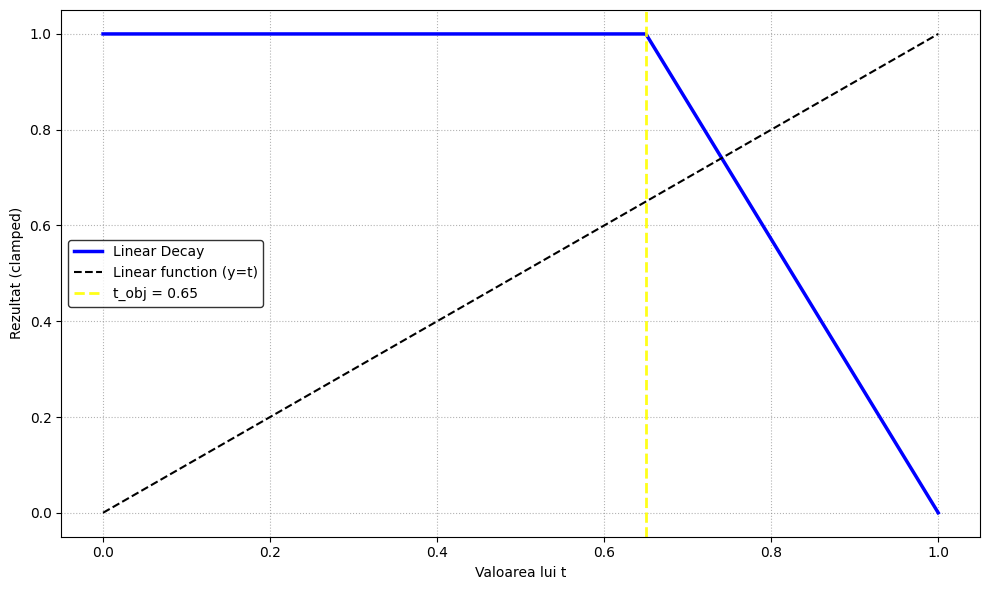
\includegraphics[width=\textwidth]{figures/linear_decay_decoding.png}
        \caption{Linear Decay}
        \label{fig:linear}
    \end{subfigure}
    \hfill
    \begin{subfigure}[b]{0.32\textwidth}
        \centering
        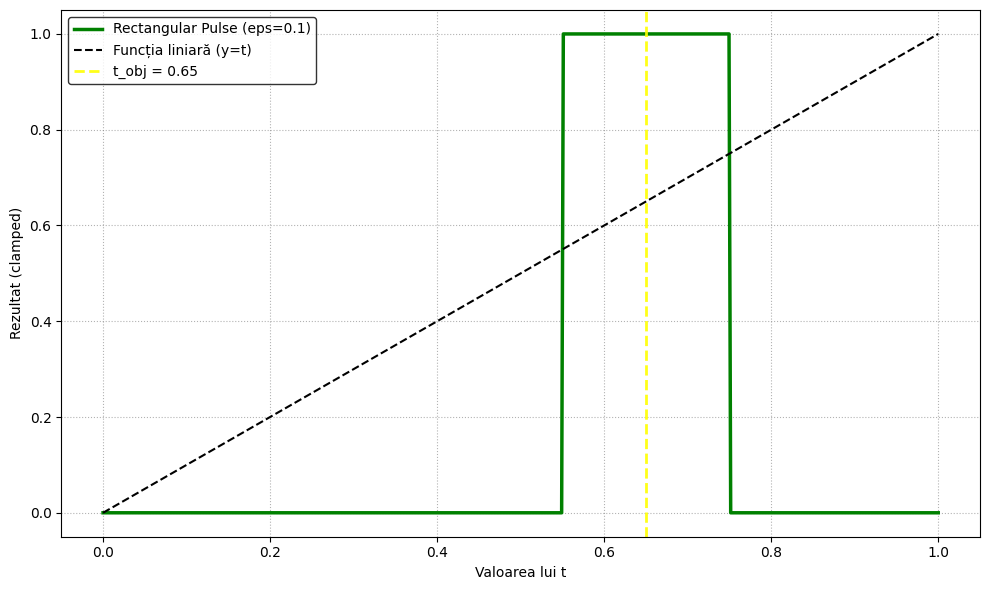
\includegraphics[width=\textwidth]{figures/rectangular_pulse_decoding.png}
        \caption{Rectangular Pulse}
        \label{fig:pulse}
    \end{subfigure}
    \hfill
    \begin{subfigure}[b]{0.32\textwidth}
        \centering
        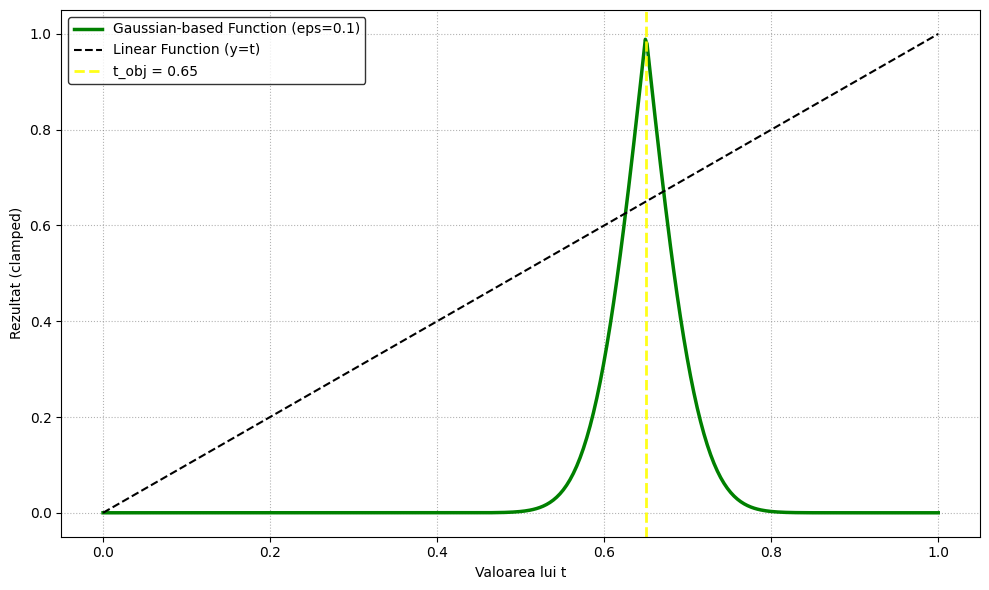
\includegraphics[width=\textwidth]{figures/gaussian-based-decoding.png}
        \caption{Gaussian-based}
        \label{fig:gaussian}
    \end{subfigure}
    \caption{Vizualizarea comparativă a funcțiilor de decodificare utilizate.}
    \label{fig:metode_decoding}
\end{figure}

\subsection*{Decodificarea Linear Decay}
\label{subsection:linear_decay}
Această metodă, ilustrată în Figura \ref{fig:linear}, aplică o descreștere constantă a importanței semnalului pe măsură ce timpul $t$ avansează dincolo de pragul $t_{obj}$. Ea a fost selectată pentru eficiența sa computațională și pentru capacitatea de a modela degradarea simplă a memoriei pe termen scurt a neuronilor, oferind o penalizare proporțională pentru spike-urile care apar târziu în fereastra de procesare a expresiei faciale.

\subsection*{Decodificarea Rectangular Pulse}
Metoda Rectangular Pulse (Figura \ref{fig:pulse}) acționează ca un filtru binar de tip "fereastră". Aceasta atribuie o importanță maximă (1.0) tuturor spike-urilor care apar într-un interval strict de $\pm 0.1$ față de centrul $t_{obj}$, ignorând complet restul activității. Această abordare este utilă pentru detectarea coincidențelor temporale rigide, eliminând zgomotul de fond și spike-urile izolate care nu se încadrează în dinamica temporală specifică unei anumite micro-expresii.

\subsection*{Decodificarea gaussiană (Gaussian-based Importance)}
Cea mai sofisticată metodă, bazată pe funcția de eroare ($\text{erf}$), generează o curbă de tip clopot centrată pe $t_{obj}$ (Figura \ref{fig:gaussian}). Spre deosebire de metodele anterioare, aceasta aproximează cel mai bine variabilitatea biologică a neuronilor și oferă o tranziție lină (smooth transition), fiind robustă la mici variații temporale.

\section*{Concluzii}
Acest capitol a oferit o analiză riguroasă a fundamentelor teoretice, marcând tranziția de la algoritmii clasici de învățare automată și rețelele din a doua generație (CNN, LSTM) către paradigma neuromorfică a rețelelor cu impulsuri (SNN). Prin detalierea modelului de neuron \textit{Integrate-and-Fire}, a filtrelor bio-inspirate DoG, a strategiilor de codificare neurală și a mecanismelor de plasticitate sinaptică (STDP, auto-inhibiția și homeostazia), s-a conturat un cadru conceptual robust și unitar. Cu aceste noțiuni fundamentale clar definite, sunt asigurate toate premisele necesare pentru implementarea arhitecturii propuse de tip CSNN. În cadrul etapelor următoare, acest ansamblu teoretic va fi transpus într-un pipeline experimental aplicat pe sec\-ven\-țe\-le video din setul de date CK+, permițând evaluarea sistematică și validarea comparativă atât a performanței diverselor scheme de eșantionare spațio-temporală (3D sampling), cât și a mai multor tipuri de arhitecturi în sarcina de re\-cu\-noaș\-te\-re a expresiilor faciale.
\chapter{Experimente și analiza rezultatelor}

\section{Setul de date}

În cadrul acestui proiect, pentru evaluarea performanței modelului propus, a fost utilizat setul de date \textbf{CK+ (Cohn-Kanade Extended Dataset)}, unul dintre cele mai utilizate seturi de date publice pentru recunoașterea expresiilor faciale în mediul controlat.

\subsection*{Descrierea datelor}
Setul de date CK+ conține înregistrări faciale reale, fiind compus din secvențe video ce surprind trecerea de la o expresie neutră la vârful (apexul) unei emoții specifice. 
Link-ul oficial pentru accesarea setului de date este: \url{http://www.pitt.edu/~emotion/ck-spread.htm}.

Caracteristicile principale ale subsetului utilizat sunt:
\begin{itemize}
	\item \textbf{Categorii:} Există 7 clase de emoții etichetate: 1. Furie (Anger), 2. Dispreț (Contempt), 3. Dezgust (Disgust), 4. Frică (Fear), 5. Fericire (Happiness), 6. Tristețe (Sadness), 7. Surpriză (Surprise).
	\item \textbf{Structura secvențelor:} Pentru fiecare subiect și fiecare ipostază, au fost extrase câte 10 cadre (frames), care acoperă evoluția temporală a expresiei.
	\item \textbf{Dimensiune imagini:} Imaginile au fost redimensionate la o rezoluție de $48 \times 48$ pixeli pentru a optimiza procesul de calcul.
\end{itemize}

\subsection*{Distribuția datelor pe fold-uri}
Pentru a asigura o evaluare robustă, s-a utilizat o strategie de \textbf{10-fold cross-validation}, folosind seed-ul 42 pentru reproductibilitate. Distribuția celor 309 secvențe pe cele 10 fold-uri este prezentată în Tabelul \ref{tab:distributie_date}.

\begin{table}[h!]
	\centering
	\caption{Distribuția emoțiilor pe cele 10 fold-uri (CK+)}
	\label{tab:distributie_date}
	\begin{tabular}{@{}ccccccccc@{}}
		\toprule
		\textbf{Fold} & \textbf{Anger} & \textbf{Contempt} & \textbf{Disgust} & \textbf{Fear} & \textbf{Happiness} & \textbf{Sadness} & \textbf{Surprise} & \textbf{Total} \\ \midrule
		1 & 5 & 2 & 6 & 3 & 7 & 3 & 8 & 34 \\
		2 & 5 & 2 & 6 & 3 & 7 & 3 & 8 & 34 \\
		3 & 5 & 1 & 6 & 3 & 7 & 3 & 8 & 33 \\
		4 & 5 & 1 & 6 & 3 & 7 & 3 & 8 & 33 \\
		5 & 5 & 1 & 5 & 2 & 7 & 3 & 8 & 31 \\
		6 & 4 & 1 & 5 & 2 & 7 & 3 & 8 & 30 \\
		7 & 4 & 1 & 5 & 2 & 7 & 3 & 8 & 30 \\
		8 & 4 & 1 & 5 & 2 & 7 & 3 & 7 & 29 \\
		9 & 4 & 1 & 5 & 2 & 7 & 2 & 7 & 28 \\
		10 & 4 & 1 & 5 & 2 & 6 & 2 & 7 & 27 \\ \midrule
		\textbf{Total} & \textbf{45} & \textbf{12} & \textbf{54} & \textbf{24} & \textbf{69} & \textbf{28} & \textbf{77} & \textbf{309} \\ \bottomrule
	\end{tabular}
\end{table}

\section{Metodologie de antrenare și evaluare}

\subsection*{Arhitectura modelului și paradigma de învățare}
Modelul implementat se bazează pe o rețea neuronală cu impulsuri (\textit{Spiking Neural Network} - SNN) cu o arhitectură convoluțională 3D, capabilă să proceseze atât informația spațială, cât și pe cea temporală din secvențele video.

Paradigma de învățare utilizată este una de tip \textbf{STDP (Spike-Timing-Dependent Plasticity)}, specific regula \textit{Biological STDP}. Aceasta permite ajustarea greutăților sinaptice în funcție de corelația temporală a impulsurilor dintre neuronii pre-sinaptici și post-sinaptici.

\subsection*{Preprocesarea datelor}
Înainte de a fi introduse în rețea, datele trec prin următoarele etape:
\begin{enumerate}
	\item \textbf{Filtrare On/Off:} Utilizarea unui \texttt{DefaultOnOffFilter} pentru evidențierea contrastelor și a marginilor (mărime filtru 7, parametri 0.1 și 1.0).
	\item \textbf{MaxScaling:} Normalizarea intensității pixelilor.
	\item \textbf{Latency Coding:} Conversia pixelilor în impulsuri (spikes), unde intensitatea este codificată prin latența temporală a primului impuls.
\end{enumerate}

\subsection*{Configurarea stratului convoluțional și hiper-parametri}
Nucleul modelului este reprezentat de un strat de convoluție 3D (\texttt{Convolution3D}). Parametrii utilizați pentru antrenare sunt detaliați în Tabelul \ref{tab:hiperparametri}.

\begin{table}[h!]
	\centering
	\caption{Hiper-parametrii rețelei SNN}
	\label{tab:hiperparametri}
	\begin{tabular}{ll}
		\toprule
		\textbf{Parametru} & \textbf{Valoare} \\ \midrule
		Număr de filtre & 64 \\
		Dimensiune filtru (WxHxD) & $5 \times 5 \times 3$ \\
		Număr de epoci & 800 \\
		Threshold inițial ($\theta$) & 4.0 \\
		$t_{obj}$ (Time Objective) & 0.80 \\
		Learning rate Threshold ($\mu_{th}$) & 0.09 \\
		Learning rate Greutăți ($\mu_{w}$) & 0.009 \\
		Spatial Pooling (output size) & $4 \times 4$ \\
		Temporal Pooling (output size) & 2 \\
		\bottomrule
	\end{tabular}
\end{table}

\subsection*{Evaluarea și Clasificarea}
După extragerea trăsăturilor prin stratul convoluțional SNN și aplicarea metodelor de \textit{SumPooling} și \textit{TemporalPooling}, reprezentările finale sunt clasificate folosind un algoritm \textbf{SVM (Support Vector Machine)}. Evaluarea se face prin cross-validation pe cele 10 fold-uri menționate anterior.

\section{Metrici de evaluare}

\begin{itemize}\item \textbf{Metrici Globale de Clasificare:}\begin{itemize}\item \textbf{Acuratețea (Accuracy):} Proporția predicțiilor corecte din totalul eșantioanelor:
		
		\[ \text{Accuracy} = \frac{N_{correct}}{N_{total}} \times 100\% \]
		
		\textbf{Matricea de Confuzie:} Reprezentare tabelară pentru identificarea erorilor sistematice între emoții similare (ex. \textit{fear} vs \textit{surprise}).\end{itemize}
	
	\item \textbf{Metrici Specifice Straturilor SNN (Per Layer Analysis):}
	\begin{itemize}
		\item \textbf{Activitatea Neuronală (Activity):} Reprezintă rata de declanșare a spike-urilor în cadrul stratului. 
		\begin{itemize}
			\item \textit{Importanță:} Un neuron care emite un spike tinde să își reducă la tăcere vecinii (inhibiție laterală). Analiza activității este esențială pentru menținerea stării de \textbf{homeostazie} a rețelei.
		\end{itemize}
		\item \textbf{Coerența (Coherence):} Măsoară gradul de redundanță al trăsăturilor învățate. 
		\begin{itemize}
			\item \textit{Interpretare:} O coerență scăzută indică faptul că SNN-ul a învățat o varietate mare de trăsături distincte. Antrenamentul eficient trebuie să tindă spre o anumită \textbf{incoerență} pentru a maximiza capacitatea de reprezentare.
		\end{itemize}
	\end{itemize}
\end{itemize}

\subsubsection{Activitatea Neuronală (Activity)}
Reprezintă dinamica de descărcare a spike-urilor în raport cu topologia stratului.

\begin{itemize}
	\item \textbf{Sparsity (Raritatea):} Se calculează pe baza raportului dintre norma $L_1$ și norma $L_2$ a activărilor. 
	\begin{itemize}
		\item \textit{Interval optim:} O valoare cuprinsă între \textbf{0.7 și 0.9} este ideală. O raritate prea mare (spre 1.0) indică o rețea "moartă", în timp ce o valoare mică indică o activitate densă, care anulează avantajul energetic al SNN.
	\end{itemize}
	\item \textbf{Active Units (\%):} Procentul de neuroni care emit cel puțin un spike per eșantion.
	\begin{itemize}
		\item \textit{Interval optim:} Pentru straturi convoluționale, o activitate de \textbf{1\% - 5\%} este considerată biologic plauzibilă și eficientă computațional.
	\end{itemize}
	\item \textbf{Quiet (\%):} Procentul de eșantioane pentru care stratul nu a generat niciun spike.
	\begin{itemize}
		\item \textit{Interpretare:} Această valoare trebuie să fie cât mai aproape de \textbf{0\%}. O valoare ridicată (ex. >10\%) sugerează că pragul de activare (\textit{threshold}) este prea înalt sau că datele de intrare nu sunt normalizate corect.
	\end{itemize}
\end{itemize}

\subsubsection{Coerența Trăsăturilor (Coherence)}
Măsoară similitudinea spectrală între nucleele (kernel-urile) de convoluție prin calcularea similitudinii cosinus între vectorii de ponderi $w_i$ și $w_j$.

\begin{equation}
	\text{Coherence}(w_i, w_j) = \frac{w_i \cdot w_j}{\|w_i\| \|w_j\| + \epsilon}
\end{equation}

\begin{itemize}
	\item \textbf{Interpretarea Cuartilelor (Q1, Q2, Q3):}
	\begin{itemize}
		\item \textit{Interval optim (Mediana/Q2):} O valoare sub \textbf{0.3 - 0.5} indică o rețea sănătoasă care a învățat trăsături diverse (margini, texturi diferite). 
		\item \textit{Riscuri:} Dacă \textit{Max} și \textit{Q3} tind spre \textbf{0.9 - 1.0}, rețeaua suferă de redundanță extremă (mai mulți neuroni au învățat exact aceeași trăsătură), ceea ce limitează capacitatea de discriminare a emoțiilor.
	\end{itemize}
	\item \textbf{Importanța Incoerenței:} Un grad ridicat de decorelare între filtre este esențial pentru ca algoritmul de clasificare ulterior (SVM sau FC) să poată extrage informație utilă din spațiul trăsăturilor.
\end{itemize}


\section{Rezultate obținute și analiză}

În această secțiune sunt prezentate performanțele obținute în urma procesului de cross-validation, precum și o analiză detaliată a comportamentului rețelei la nivel de distribuție a datelor și a impulsurilor (\textit{spikes}).

\subsection*{Performanța pe fold-uri}

Rezultatele clasificării pentru fiecare dintre cele 10 fold-uri sunt centralizate în Tabelul \ref{tab:rezultate_folds}. Rata medie de clasificare obținută este de aproximativ \textbf{48.02\%}.

\begin{table}[h!]
	\centering
	\caption{Acuratețea clasificării pe fiecare fold}
	\label{tab:rezultate_folds}
	\begin{tabular}{@{}ccc@{}}
		\toprule
		\textbf{Fold} & \textbf{Rata de clasificare (\%)} & \textbf{Corecte / Total} \\ \midrule
		Fold 1 & 58.82\% & 20/34 \\
		Fold 2 & 47.05\% & 16/34 \\
		Fold 3 & 51.51\% & 17/33 \\
		Fold 4 & 45.45\% & 15/33 \\
		Fold 5 & 41.93\% & 13/31 \\
		Fold 6 & 53.33\% & 16/30 \\
		Fold 7 & 50.00\% & 15/30 \\
		Fold 8 & 48.27\% & 14/29 \\
		Fold 9 & 35.71\% & 10/28 \\
		Fold 10 & 48.14\% & 13/27 \\ \midrule
		\textbf{Medie} & \textbf{48.02\%} & \textbf{159 / 309} \\ \bottomrule
	\end{tabular}
\end{table}

\subsection*{Analiza detaliată pe Fold 1}
Fold-ul 1 a înregistrat cea mai ridicată performanță (58.82\%). Pentru a înțelege punctele forte și limitările modelului, matricea de confuzie pentru Fold 1 (Tabelul \ref{tab:confusion_matrix}), surprinde corelarea etichetelor reale (\textit{True Label}) cu probabilitățile maxime generate de clasificatorul SVM.

\begin{table}[h!]
	\centering
	\caption{Matricea de confuzie pentru Fold 1 (34 secvențe)}
	\label{tab:confusion_matrix}
	\begin{tabular}{r|ccccccc|c}
		\toprule
		\textbf{Real \textbackslash Prezis} & \textbf{1} & \textbf{2} & \textbf{3} & \textbf{4} & \textbf{5} & \textbf{6} & \textbf{7} & \textbf{Recall \%} \\ \midrule
		\textbf{1 (Anger)}     & 0 & 0 & 5 & 0 & 0 & 0 & 0 & 0.0\% \\
		\textbf{2 (Contempt)}  & 1 & 0 & 1 & 0 & 0 & 0 & 0 & 0.0\% \\
		\textbf{3 (Disgust)}   & 0 & 0 & \textbf{6} & 0 & 0 & 0 & 0 & 100.0\% \\
		\textbf{4 (Fear)}      & 0 & 0 & 0 & 0 & 0 & 0 & 3 & 0.0\% \\
		\textbf{5 (Happiness)} & 0 & 0 & 0 & 0 & \textbf{7} & 0 & 0 & 100.0\% \\
		\textbf{6 (Sadness)}   & 1 & 0 & 2 & 0 & 0 & 0 & 0 & 0.0\% \\
		\textbf{7 (Surprise)}  & 0 & 0 & 1 & 0 & 0 & 0 & \textbf{7} & 87.5\% \\ \midrule
		\textbf{Precision \%}  & 0.0\% & 0.0\% & 40.0\% & 0.0\% & 100.0\% & 0.0\% & 70.0\% & \textbf{Acc: 58.8\%} \\
		\bottomrule
	\end{tabular}
\end{table}

\subsubsection{Interpretarea erorilor de clasificare}
Analiza probabilităților individuale relevă câteva fenomene tipice pentru procesarea imaginilor faciale prin SNN:

\begin{itemize}
	\item \textbf{Suprapunerea caracteristicilor Furie-Dezgust:} Toate secvențele de \textit{Anger} (clasa 1) au primit probabilitatea maximă pentru \textit{Disgust} (clasa 3). Acest lucru se explică prin similitudinea morfologică a acestor expresii (încrețirea nasului și coborârea sprâncenelor), pe care filtrele convoluționale actuale le extrag ca fiind identice.
	\item \textbf{Dificultatea detectării Fricii:} Emoția \textit{Fear} (clasa 4) a fost clasificată sistematic drept \textit{Surprise} (clasa 7). Din punct de vedere vizual, ambele emoții implică deschiderea largă a ochilor și ridicarea sprâncenelor. Rezultatele sugerează că modelul reușește să detecteze activarea musculară, dar nu și subtilitatea temporală care diferențiază frica de surpriză.
	\item \textbf{Performanță Robustă la Emoții Extreme:} Clasele \textit{Happiness} și \textit{Disgust} au un \textit{recall} de 100\%, indicând faptul că arhitectura SNN propusă este extrem de eficientă în izolarea trăsăturilor de intensitate mare (zâmbet larg, respectiv contracție nazală pronunțată).
	\item \textbf{Clasele sub-reprezentate:} \textit{Contempt} și \textit{Sadness} au înregistrat performanțe slabe, fiind confundate cu emoții negative mai „puternice”. Aceasta este o limitare cunoscută a setului de date CK+, unde aceste clase au mult mai puține exemple de antrenament.
\end{itemize}

\subsection*{Analiza distribuției valorilor și a impulsurilor}
Pentru a înțelege modul în care stratul convoluțional procesează informația, am extras distribuția globală a valorilor înainte și după aplicarea stratului de convoluție 3D.

\subsubsection{Distribuția după Latency Encoding (Input)}
În faza de preprocesare, valorile sunt codificate temporal. Distribuția prezentată în Tabelul \ref{tab:dist_input} arată o concentrație masivă a valorilor în intervalul $[0.9 - 1.0]$ (peste 72\%), ceea ce indică faptul că majoritatea neuronilor de intrare generează impulsuri cu latență mare.

\subsubsection{Distribuția după Stratul Convoluțional (Spikes)}
După trecerea prin stratul de convoluție, se observă o menținere a densității în zona superioară, dar cu o ușoară redistribuire. Această activitate intensă în intervalul $[0.8 - 1.0]$ sugerează că filtrele convoluționale au identificat numeroase corelații spațio-temporale în secvențele video de intrare.

\begin{table}[h!]
	\centering
	\caption{Analiza comparativă a distribuției valorilor (Fold 1)}
	\label{tab:dist_input}
	\begin{tabular}{@{}ccc@{}}
		\toprule
		\textbf{Interval} & \textbf{Înainte de Conv (Input) \%} & \textbf{După Conv (Spikes) \%} \\ \midrule
		$[0.0 - 0.5]$ & 1.66\% & 0.01\% \\
		$[0.5 - 0.6]$ & 1.71\% & 0.14\% \\
		$[0.6 - 0.7]$ & 3.37\% & 1.24\% \\
		$[0.7 - 0.8]$ & 6.57\% & 6.34\% \\
		$[0.8 - 0.9]$ & 14.01\% & 22.49\% \\
		$[0.9 - 1.0]$ & 72.68\% & 69.78\% \\ \bottomrule
	\end{tabular}
\end{table}

\subsection*{Interpretarea rezultatelor}
Analiza distribuției arată că rețeaua nu suferă de \textit{vanishing spikes}, având o activitate susținută. Totuși, rata de clasificare medie sugerează că, deși anumite emoții cu trăsături faciale distincte (precum fericirea sau surpriza) sunt ușor de separat, distincția între emoțiile subtile (furie vs. dezgust) necesită o rafinare a hiper-parametrilor sau o creștere a numărului de filtre pentru a surprinde diferențe mai fine de textură și mișcare.
Deși rata medie de 48.02\% indică un potențial ridicat pentru recunoașterea emoțiilor de intensitate mare (Happiness, Disgust), se observă o dificultate în discriminarea stărilor afective subtile. Această limitare este pusă pe seama numărului redus de eșantioane pentru clase precum Contempt, dar și pe natura nesupervizată a algoritmului STDP, care prioritizează frecvența trăsăturilor în detrimentul discriminabilității lor. Optimizarea viitoare a pragului de activare ($\theta$) și a ratei de învățare a pragului ($\mu_{th}$) ar putea conduce la o mai bună specializare a filtrelor.

\subsection*{Vizualizarea și analiza hărților de trăsături (Feature Maps)}

Pentru a investiga modul în care modelul \textit{Convolutional SNN} extrage informația din secvențele video, au fost vizualizate hărțile de trăsături (\textit{feature maps}) generate de stratul convoluțional. Această analiză este esențială pentru a valida capacitatea regulii de învățare STDP de a codifica tipare spațio-temporale relevante fără supraveghere.

\subsubsection{Impactul mecanismului TimeObjectiveOutput}

O componentă critică în arhitectura propusă este etapa de conversie a output-ului. În Figura \ref{fig:anger_before_after} este ilustrat efectul aplicării transformării \texttt{OutputConverter.TimeObjectiveOutput} asupra unei secvențe de \textit{Anger}.

\begin{figure}[h!]
	\centering
	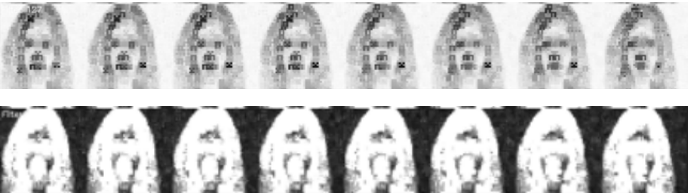
\includegraphics[width=0.9\textwidth]{figures/models/feature_maps_csnn/selection/anger-before-after.png}
	\caption{Vizualizarea hărților de trăsături pentru clasa Anger: Sus - activări brute (pre-procesare); Jos - activări după aplicarea TimeObjectiveOutput.}
	\label{fig:anger_before_after}
\end{figure}

Analiza vizuală relevă următoarele aspecte:
\begin{itemize}
	\item \textbf{Normalizarea Latenței:} În varianta brută, activările sunt difuze, având un raport semnal-zgomot scăzut. Aplicarea \texttt{TimeObjectiveOutput} forțează latențele spre valoarea țintă $t_{obj}=0.8$, rezultând într-o reprezentare mult mai clară a contururilor faciale.
	\item \textbf{Evidențierea Dinamicii:} După procesare, se observă o focalizare a impulsurilor în zonele cu mișcare musculară intensă (frunte, ochi, gură). Această „curățare” a semnalului permite clasificatorului SVM să lucreze cu trăsături mai bine definite, minimizând redundanța spațială.
\end{itemize}

\subsection*{Analiza calitativă a hărților de trăsături per emoție}

În Figurile \ref{fig:fmaps_1} și \ref{fig:fmaps_2} sunt prezentate seturile de hărți de trăsături extrase pentru cele 7 categorii de emoții. Fiecare eșantion este reprezentat printr-o succesiune de cadre ce reflectă intensitatea activării neuronale. În paradigma \textit{Latency Coding}, zonele albe (pixeli cu intensitate mare) corespund unor latențe mici, indicând o declanșare rapidă a impulsurilor ca răspuns la trăsături faciale proeminente.

\begin{figure}[h!]
	\centering
	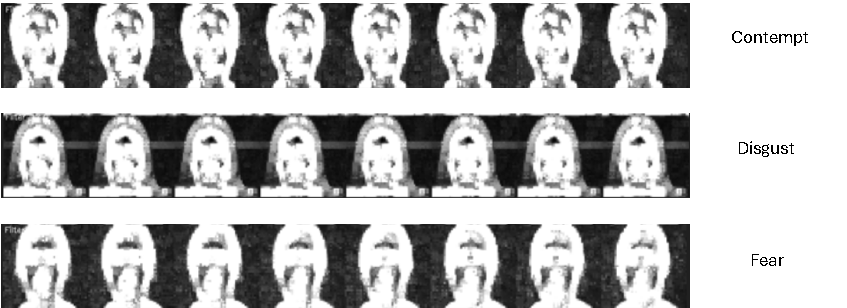
\includegraphics[width=0.85\textwidth]{figures/models/feature_maps_csnn/selection/feature-maps-1.png}
	\caption{Hărți de trăsături pentru clasele Contempt, Disgust și Fear.}
	\label{fig:fmaps_1}
\end{figure}

\begin{figure}[h!]
	\centering
	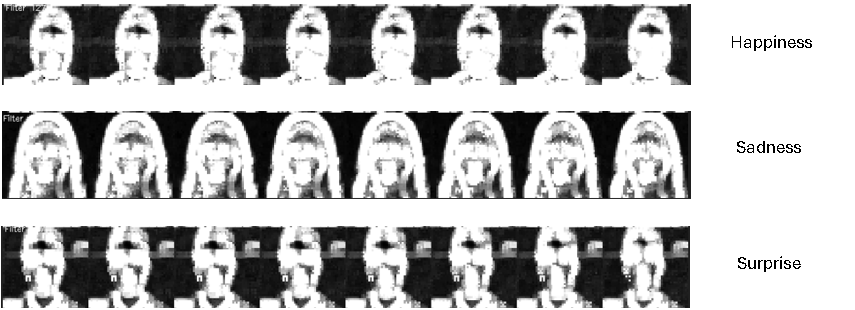
\includegraphics[width=0.85\textwidth]{figures/models/feature_maps_csnn/selection/feature-maps-2.png}
	\caption{Hărți de trăsături pentru clasele Happiness, Sadness și Surprise.}
	\label{fig:fmaps_2}
\end{figure}

\subsubsection{Corelația dintre trăsături și performanța clasificării}

Observarea hărților de trăsături permite explicarea rezultatelor obținute în matricea de confuzie:

\begin{itemize}
	\item \textbf{Happiness și Disgust:} Aceste clase prezintă zone de activare extrem de bine localizate (comisurile bucale pentru fericire și zona nazală pentru dezgust). Caracterul distinctiv al acestor impulsuri timpurii explică rata de \textit{recall} de 100\% pentru aceste clase.
	\item \textbf{Surprise vs. Fear:} Hărțile de trăsături confirmă similitudinea vizuală între cele două emoții. În ambele cazuri, filtrele SNN detectează deschiderea largă a ochilor, însă distribuția spațială a impulsurilor este aproape identică, ceea ce conduce la clasificarea sistematică a fricii drept surpriză.
	\item \textbf{Sadness și Contempt:} Aceste emoții generează hărți cu o densitate mai mică a impulsurilor („pete” mai întunecate), indicând o mișcare facială de intensitate redusă. Această activitate rarefiată face ca trăsăturile extrase să fie mai puțin robuste în fața zgomotului, explicând performanța scăzută pe aceste clase.
\end{itemize}

Această analiză vizuală demonstrează că modelul SNN propus a învățat să acționeze ca un extractor de trăsături fiziologice, reușind să mapeze corelările spațio-temporale din clipurile video în latențe neuronale discriminative.

\subsubsection{Vizualizarea nucleelor convoluționale (Greutăți Sinaptice)}

Pentru o înțelegere aprofundată a modului în care s-a realizat adaptarea sinaptică prin procesul STDP nesupervizat, au fost extrase greutățile sinaptice ale celor 64 de filtre după cele 800 de epoci de antrenament pe Fold 1. Vizualizarea acestor nuclee (\textit{kernels}) de dimensiune $5 \times 5 \times 3$ este prezentată în Figura \ref{fig:kernels_fold_1}. Deoarece un nucleu este tridimensional (spatial $5 \times 5$ pe o adâncime temporală $3$), vizualizarea este o proiecție color a volumului de greutăți.

\begin{figure}[h!]
	\centering
	% Asigură-te că imaginea ta este redenumită sau salvată sub acest nume în folderul proiectului
	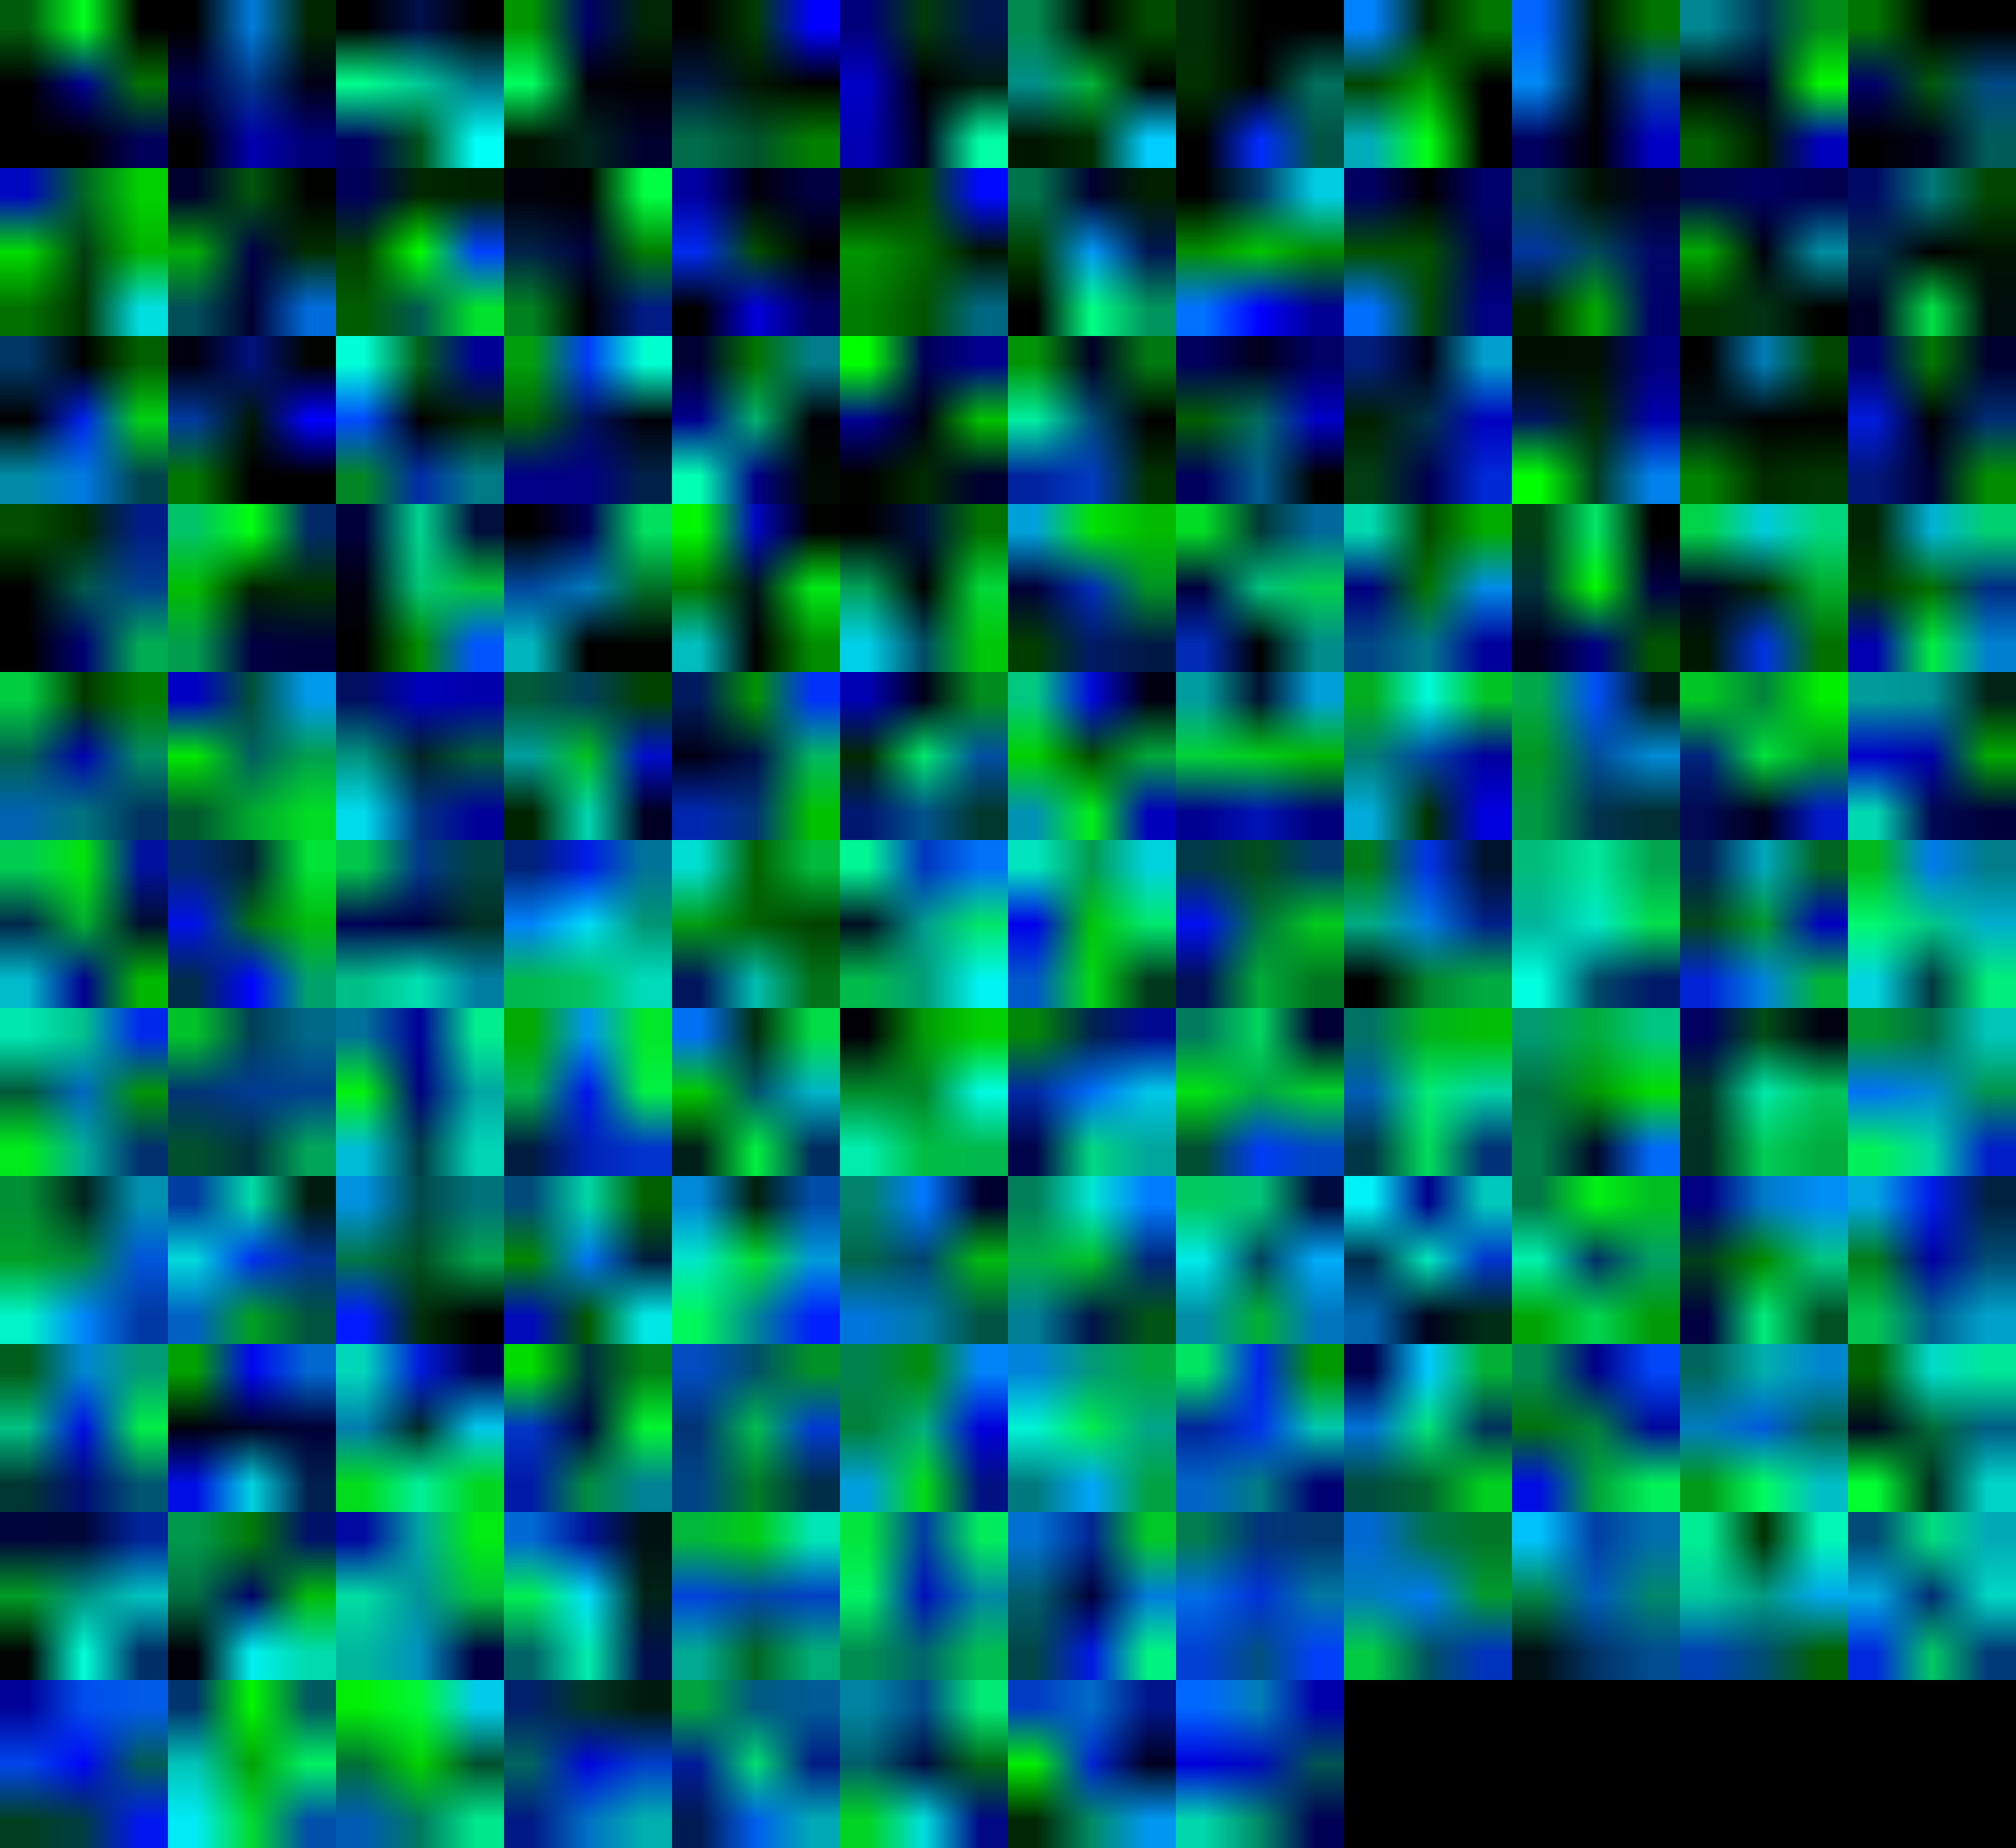
\includegraphics[width=0.6\textwidth]{figures/models/kernels_csnn/kernels_fold_1.png} 
	\caption{Vizualizarea celor 64 de nuclee convoluționale ($8 \times 8$ filtre) învățate de SNN pe Fold 1. Culoarea reprezintă magnitudinea și polaritatea greutăților sinaptice (nivele de potențiere și depresie).}
	\label{fig:kernels_fold_1}
\end{figure}

Analiza calitativă a Figura \ref{fig:kernels_fold_1} relevă tipare caracteristice învățării STDP nesupervizate pe secvențe video:

\begin{itemize}
	\item \textbf{High-Frequency Spatial Variance:} Nucleele prezintă o variație spațială ridicată, aspectul lor fiind aparent zgomotos. Acest fenomen este caracteristic etapelor inițiale de specializare a filtrelor în SNN-uri nesupervizate. În loc să învețe margini orientate generice (cum ar fi filtrele Gabor), STDP-ul tinde să specializeze nucleele pe tipare foarte locale și specifice de corelații temporale de impulsuri, prezente în datele de intrare.
	\item \textbf{Validarea Incoerenței:} Aspectul divers și aparent aleatoriu al filtrelor este, paradoxal, un rezultat dorit. Așa cum s-a menționat în secțiunea \ref{sec:metrici} (definiția coerenței), antrenamentul eficient trebuie să tindă spre o incoerență ridicată. Faptul că filtrele nu sunt identice și nu prezintă trăsături repetitive validează succesul regulii de învățare STDP în a evita redundanța și în a acoperi un spectru larg de variații ale datelor.
	\item \textbf{Limitările învățării trăsăturilor globale:} Absența unor structuri globale clar definite în kernels explică performanța scăzută pe clasele subtile. Filtrele sunt suficient de discriminate pentru a distinge între schimbări majore de intensitate (zâmbet vs. contracție nazală), dar nu au învățat încă să reprezinte deformări fine ale feței pe care clasificatorul liniar ulterior (SVM) să le poată separa eficient.
\end{itemize}

\section{Analiză Comparativă și Validarea Modelului}

Pentru a evalua relevanța trăsăturilor extrase de stratul convoluțional SNN, a fost realizat un experiment de control (baseline). În cadrul acestuia, clasificatorul SVM a fost antrenat direct pe pixelii imaginilor brute (\textit{raw pixels}), eliminând complet componenta de spiking și procesarea STDP.

\subsection*{Configurația modelului de referință (Baseline)}
Modelul de referință utilizează un strat de tip \texttt{layer::Stream}, care acționează ca o funcție identitate, pasând datele de intrare direct către etapele de pooling, fără nicio preprocesare sau filtrare temporală. Configurația utilizată este următoarea:

\begin{itemize}
	\item \textbf{Input:} Pixeli raw (fără \textit{Latency Coding}).
	\item \textbf{Pooling:} \texttt{SumPooling} ($4 \times 4$) și \texttt{TemporalPooling} (2), identic cu modelul SNN pentru a asigura o comparație echitabilă a spațiului de trăsături.
	\item \textbf{Clasificator:} SVM liniar.
\end{itemize}

\subsection*{Rezultate comparative}

Rezultatele obținute prin cross-validation pentru ambele abordări sunt centralizate în Tabelul \ref{tab:comparatie_rezultate}.

\begin{table}[h!]
	\centering
	\caption{Comparație între SVM pe pixeli raw și arhitectura propusă (SNN + SVM)}
	\label{tab:comparatie_rezultate}
	\begin{tabular}{@{}ccc@{}}
		\toprule
		\textbf{Fold} & \textbf{SVM Pixeli Raw (\%)} & \textbf{SNN + SVM (Propus) (\%)} \\ \midrule
		Fold 1 & 44.11\% & 58.82\% \\
		Fold 2 & 38.23\% & 47.05\% \\
		Fold 3 & 54.54\% & 51.51\% \\
		Fold 4 & 39.39\% & 45.45\% \\
		Fold 5 & 38.70\% & 41.93\% \\
		Fold 6 & 36.66\% & 53.33\% \\
		Fold 7 & 43.33\% & 50.00\% \\
		Fold 8 & 44.82\% & 48.27\% \\
		Fold 9 & 39.28\% & 35.71\% \\
		Fold 10 & 37.03\% & 48.14\% \\ \midrule
		\textbf{Medie} & \textbf{41.61\%} & \textbf{48.02\%} \\ \bottomrule
	\end{tabular}
\end{table}

\subsection*{Interpretarea superiorității modelului SNN}

Compararea performanțelor evidențiază un câștig net de \textbf{6.41\%} în favoarea arhitecturii bazate pe SNN. Această diferență, deși aparent modestă în cifre absolute, este semnificativă din punct de vedere al procesării bio-inspirate:

\begin{enumerate}
	\item \textbf{Extracția de trăsături (Feature Extraction):} Diferența de performanță confirmă faptul că nucleele învățate prin STDP nu sunt aleatorii; ele reușesc să distileze informația vizuală în „puncte de interes” temporale care sunt mai ușor de separat liniar de către un SVM decât pixelii bruti.
	\item \textbf{Reducerea zgomotului:} În timp ce pixelii raw conțin multă informație redundantă (fundal, variații de iluminare), SNN-ul, prin filtrarea On/Off și Latency Coding, se concentrează pe marginile dinamice (schimbările de expresie), oferind un input mai „curat” pentru clasificator.
	\item \textbf{Analiza cazurilor particulare:} Se observă că în aproape toate fold-urile (cu excepția fold-ului 3 și 9), SNN-ul depășește baseline-ul. În Fold 1, saltul este de la 44.11\% la 58.82\% (+14.71\%), ceea ce indică faptul că pentru anumite secvențe video, reprezentarea prin impulsuri este net superioară celei spațiale clasice.
\end{enumerate}

În concluzie, rezultatele demonstrează validitatea ipotezei de lucru: rețelele neuronale cu impulsuri, antrenate nesupervizat, sunt capabile să extragă trăsături temporale relevante pentru recunoașterea expresiilor faciale, îmbunătățind capacitatea de generalizare a sistemului față de procesarea directă a imaginilor.

\section{Modelul de Înaltă Performanță: Arhitectura Hibridă CNN-LSTM}

Pentru a oferi un termen de comparație raportat la standardele actuale de \textit{Deep Learning} și pentru a echipa aplicația finală cu un motor de predicție robust, a fost implementată o arhitectură hibridă de tip \textbf{CNN-LSTM}. Acest model combină puterea de extracție a trăsăturilor spațiale ale unei rețele convoluționale pre-antrenate cu capacitatea rețelelor recurente de a modela evoluția temporală a emoțiilor.

\subsection*{Descrierea Arhitecturii}

Modelul propus utilizează un mecanism de \textit{Feature Extraction} urmat de un modul de memorie temporală:
\begin{enumerate}
	\item \textbf{Extractorul Spațial (Backbone):} S-a utilizat modelul \textbf{ResNet18}, pre-antrenat pe setul de date ImageNet. S-a păstrat structura până la stratul de \textit{Adaptive Average Pooling}, rezultând un vector de trăsături de dimensiune 512 pentru fiecare cadru video.
	\item \textbf{Modulul Temporal (LSTM):} Trăsăturile extrase sunt introduse într-un strat \textbf{LSTM} (\textit{Long Short-Term Memory}) cu o dimensiune ascunsă de 256. Acesta analizează succesiunea celor 10 cadre pentru a identifica „apexul” emoției.
	\item \textbf{Capul de Clasificare:} Un modul de tip \textit{Fully Connected} cu \textit{Dropout} (0.5) și activare ReLU realizează maparea finală către cele 7 clase de emoții.
\end{enumerate}

\subsection*{Strategia de Antrenament în Două Faze}

Pentru a maximiza performanța pe un set de date de dimensiuni medii precum CK+, s-a adoptat o strategie de \textit{Transfer Learning} structurată în două etape:
\begin{itemize}
	\item \textbf{Faza 1 (Warm-up):} Înghețarea parametrilor CNN și antrenarea exclusivă a modulelor LSTM și FC timp de 10 epoci (LR=$10^{-3}$). Acest lucru permite modelului temporal să se adapteze la trăsăturile extrase de ResNet.
	\item \textbf{Faza 2 (Fine-tuning):} Dezghețarea selectivă a ultimului bloc convoluțional (\textit{Layer 4}) din ResNet și antrenarea întregului ansamblu timp de 30 de epoci cu un \textit{Learning Rate} scăzut ($10^{-4}$) și \textit{Cosine Annealing}.
\end{itemize}

\subsection*{Rezultate Obținute}

Performanța modelului CNN-LSTM, evaluată prin 10-fold cross-validation, este prezentată în Tabelul \ref{tab:rezultate_cnn_lstm}.

\begin{table}[h!]
	\centering
	\caption{Acuratețea modelului CNN-LSTM pe cele 10 fold-uri}
	\label{tab:rezultate_cnn_lstm}
	\begin{tabular}{@{}lc|lc@{}}
		\toprule
		\textbf{Fold} & \textbf{Acuratețe (\%)} & \textbf{Fold} & \textbf{Acuratețe (\%)} \\ \midrule
		Fold 1 & 87.88\% & Fold 6 & 85.71\% \\
		Fold 2 & 85.71\% & Fold 7 & 93.75\% \\
		Fold 3 & 81.82\% & Fold 8 & 89.66\% \\
		Fold 4 & 87.50\% & Fold 9 & 78.57\% \\
		Fold 5 & 96.97\% & Fold 10 & 96.15\% \\ \midrule
		\textbf{Medie} & \multicolumn{3}{c}{\textbf{88.37\% $\pm$ 5.65\%}} \\ \bottomrule
	\end{tabular}
\end{table}

\section{Sinteza Rezultatelor și Concluzii Experimentale}

În Tabelul \ref{tab:sinteza_finala} este prezentată comparația finală între cele trei abordări investigate în cadrul acestei lucrări.

\begin{table}[h!]
	\centering
	\caption{Comparație centralizată a modelelor evaluate}
	\label{tab:sinteza_finala}
	\begin{tabular}{lccc}
		\toprule
		\textbf{Model} & \textbf{Paradigmă} & \textbf{Acuratețe Medie} & \textbf{Complexitate} \\ \midrule
		SVM (Raw Pixels) & Baseline Statistic & 41.61\% & Minimă \\
		\textbf{3D Conv SNN} & Bio-inspirat (STDP) & \textbf{48.02\%} & Medie \\
		CNN-LSTM (ResNet) & Deep Learning & \textbf{88.37\%} & Ridicată \\ \bottomrule
	\end{tabular}
\end{table}

\subsection*{Discuții}
Deși modelul CNN-LSTM oferă cea mai înaltă precizie, fiind soluția optimă pentru aplicația practică de monitorizare în timp real, rezultatele obținute cu modelul \textbf{SNN} sunt promițătoare. 

Diferența de performanță este explicată prin natura învățării: în timp ce CNN-LSTM beneficiază de pre-antrenare pe milioane de imagini și învățare supervizată prin \textit{backpropagation}, modelul SNN propus utilizează o regulă de învățare locală, nesupervizată (STDP), mult mai eficientă din punct de vedere energetic și biologic. Această lucrare demonstrează că SNN-ul poate extrage trăsături relevante care depășesc performanța unui clasificator liniar aplicat pe date brute, deschizând calea către sisteme de recunoaștere a emoțiilor implementabile pe hardware neuromorfic.

\subsection*{Preprocesare și Augmentarea Datelor}

Pentru modelul CNN-LSTM, strategia de pregătire a datelor a fost semnificativ mai complexă față de abordările SNN și SVM. Antrenarea s-a realizat exclusiv pe imagini focalizate strict pe zona feței (\textit{cropped faces}), eliminând astfel elementele de fundal care ar fi putut introduce zgomot în procesul de extracție a trăsăturilor.

Spre deosebire de experimentele anterioare, unde s-au utilizat preprocesări minimale, aici s-a implementat o conductă de \textbf{augmentare a datelor} pentru a îmbunătăți generalizarea și a combate supra-antrenarea (\textit{overfitting}). Deoarece setul CK+ este monocrom, cadrele au fost convertite la 3 canale (RGB) pentru a fi compatibile cu arhitectura ResNet18, aplicându-se următoarele transformări: Resize(224, 224), Grayscale(num\_output\_channels=3), RandomHorizontalFlip(), RandomRotation(10), ColorJitter(brightness=0.2, contrast=0.2), Normalize([0.485, 0.456, 0.406], [0.229, 0.224, 0.225]).

\subsection*{Analiza performanței pe Fold 5}

Analiza detaliată a Fold-ului 5 relevă eficiența modelului CNN-LSTM, acesta obținând o acuratețe de 96.97\%. În Figura \ref{fig:cm_fold5} se poate observa că modelul a reușit să clasifice perfect 6 din cele 7 emoții.

\begin{figure}[h!]
	\centering
	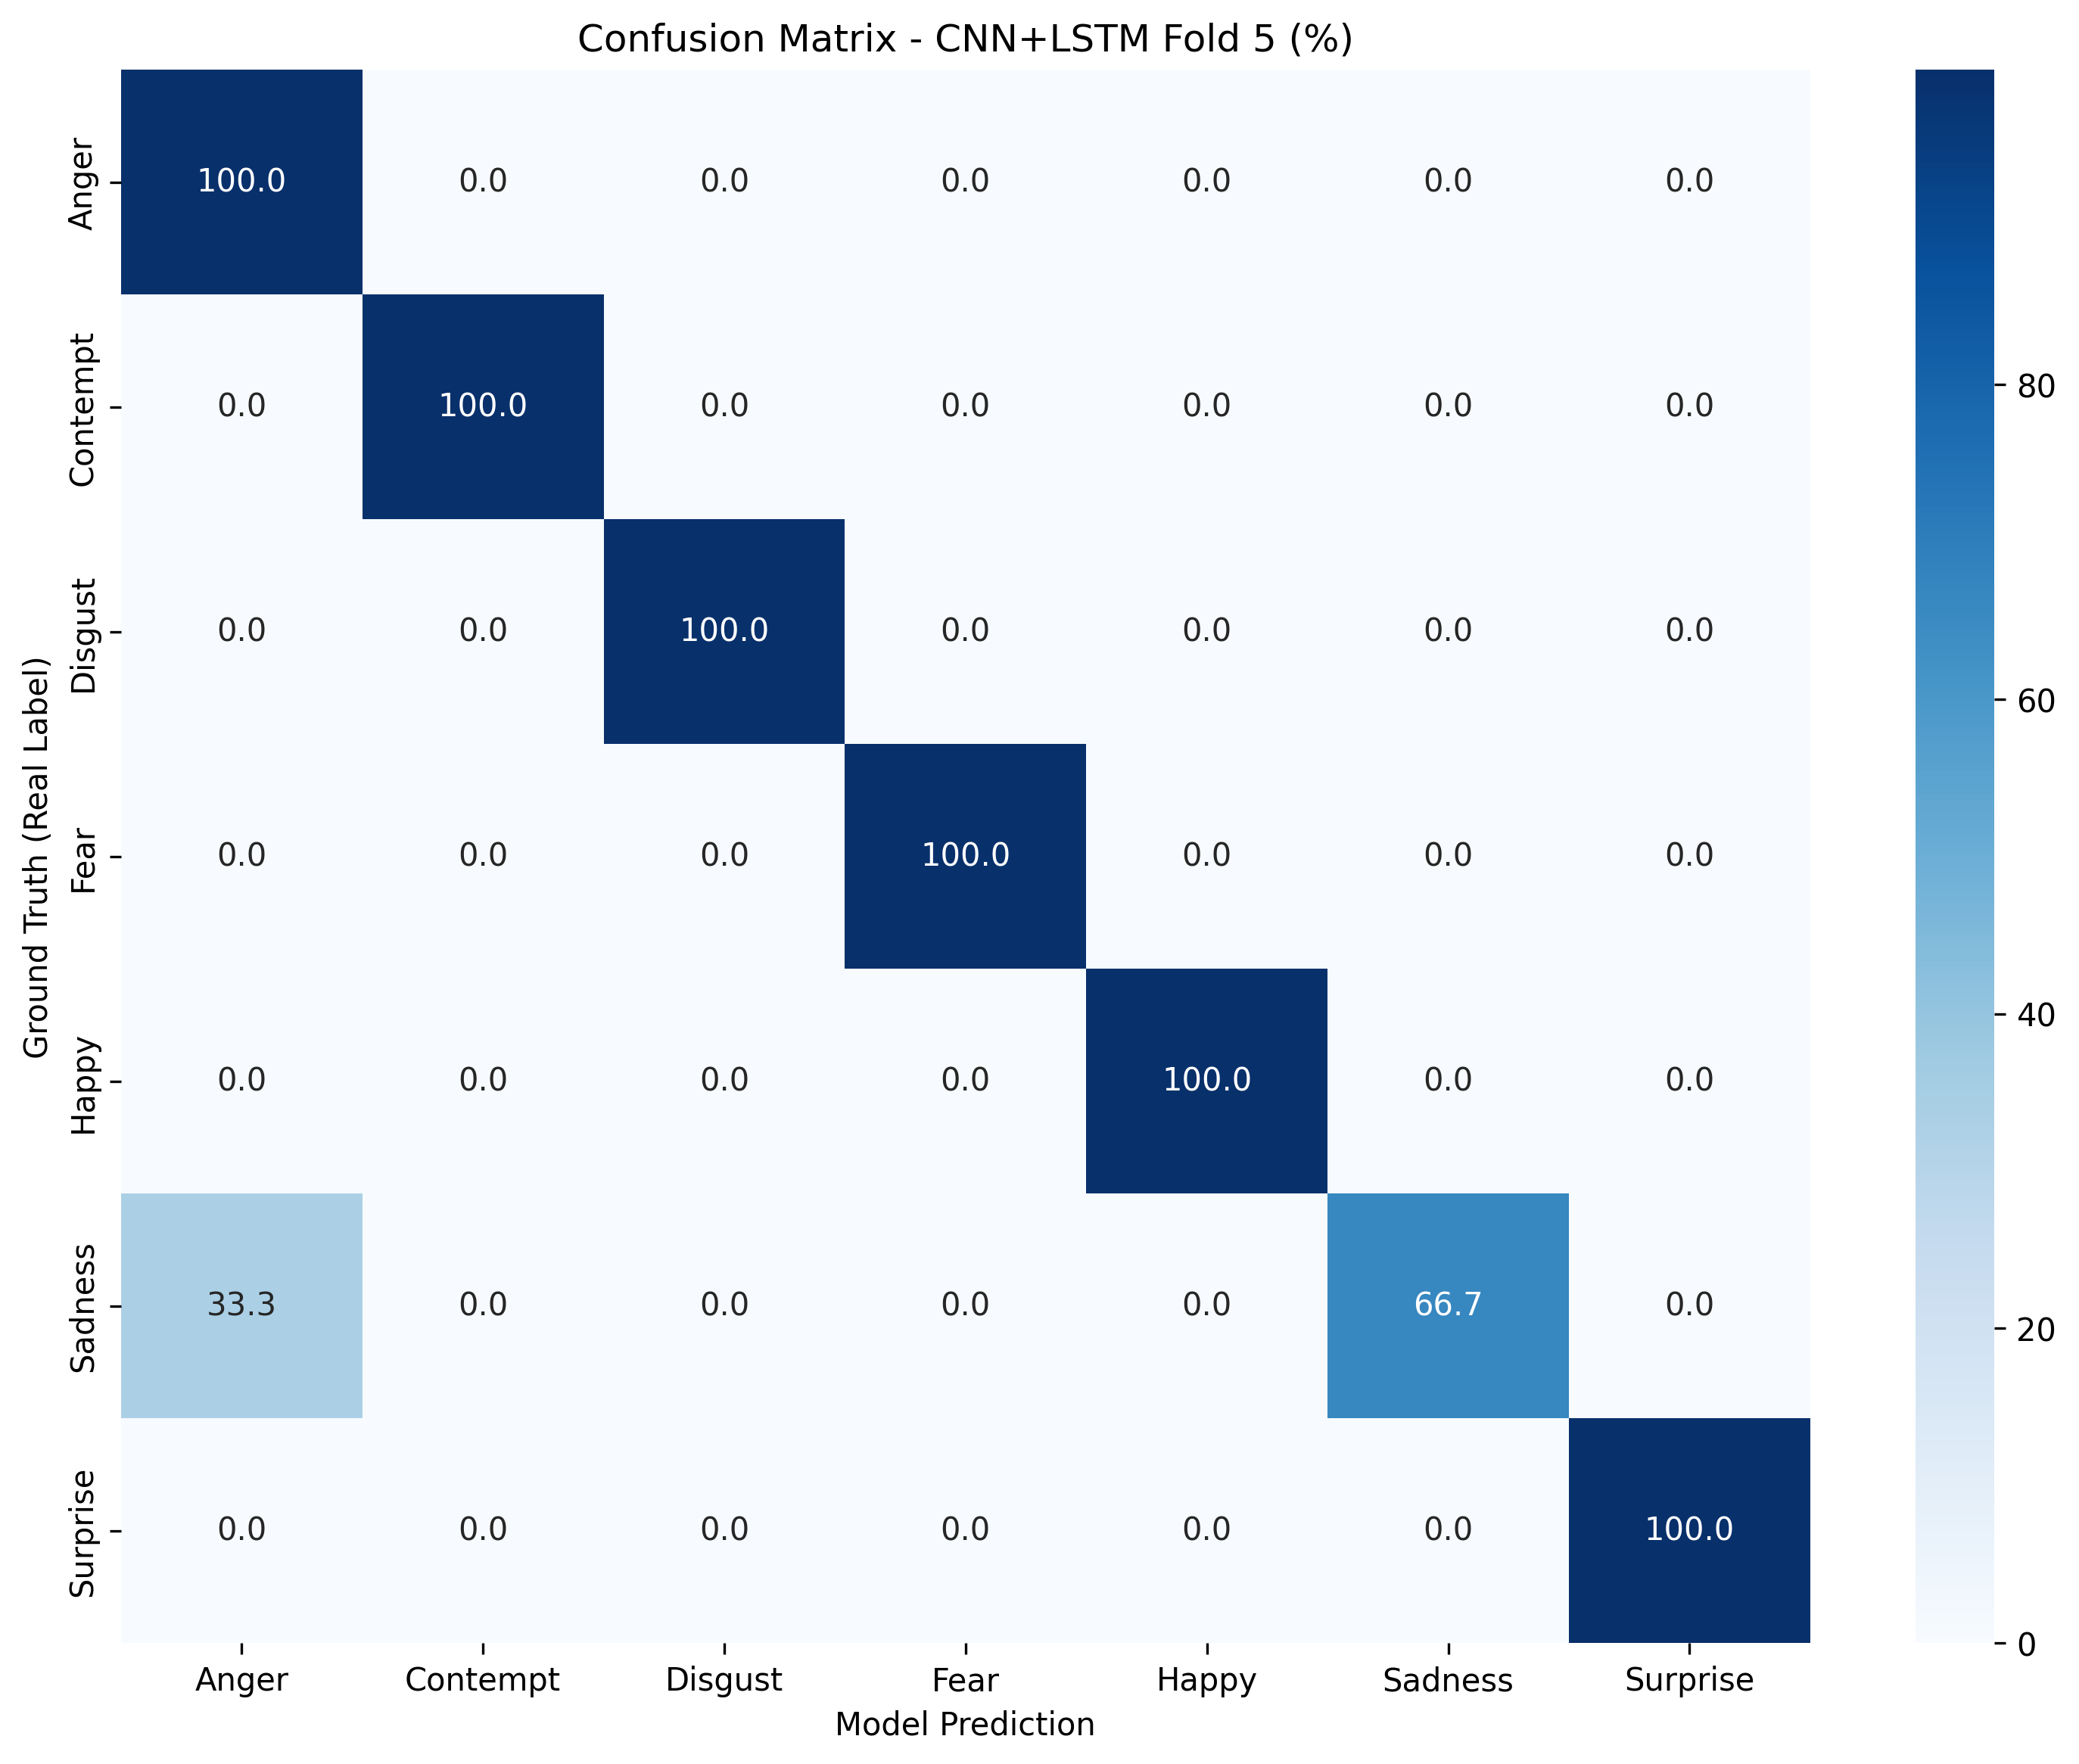
\includegraphics[width=0.7\textwidth]{figures/models/confusion_matrix_fold_5.png}
	\caption{Matricea de confuzie pentru CNN-LSTM (Fold 5). Se observă o singură eroare de clasificare.}
	\label{fig:cm_fold5}
\end{figure}

Singura eroare înregistrată a fost un eșantion din clasa \textbf{Sadness}, care a fost identificat eronat ca fiind \textbf{Anger}. Această confuzie este explicabilă prin tensiunea musculară similară în zona sprâncenelor (coborârea acestora) prezentă în ambele expresii în stadiul de apex.

\subsection*{Interpretarea deciziilor prin Grad-CAM}

Pentru a valida calitativ modelul, s-a utilizat tehnica \textbf{Grad-CAM (Gradient-weighted Class Activation Mapping)}. Aceasta permite vizualizarea zonelor feței pe care rețeaua s-a focalizat pentru a stabili eticheta emoțională. În Figura \ref{fig:gradcam_grid} sunt prezentate hărțile de activare pentru eșantioanele din Fold 5.

\begin{figure}[h!]
	\centering
	\begin{subfigure}{0.24\textwidth}
		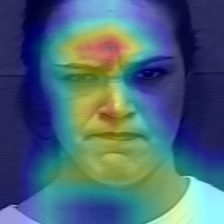
\includegraphics[width=\textwidth]{figures/models/gradcam_cnn+lstm_fold5/anger_pass.jpg}
		\caption{Anger}
	\end{subfigure}
	\begin{subfigure}{0.24\textwidth}
		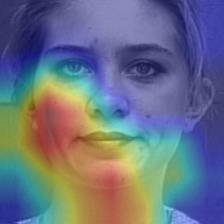
\includegraphics[width=\textwidth]{figures/models/gradcam_cnn+lstm_fold5/contempt_pass.jpg}
		\caption{Contempt}
	\end{subfigure}
	\begin{subfigure}{0.24\textwidth}
		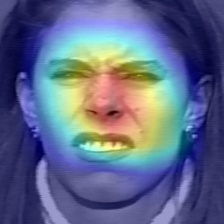
\includegraphics[width=\textwidth]{figures/models/gradcam_cnn+lstm_fold5/disgust_pass.jpg}
		\caption{Disgust}
	\end{subfigure}
	\begin{subfigure}{0.24\textwidth}
		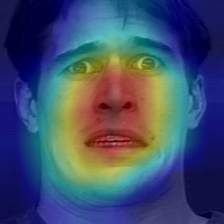
\includegraphics[width=\textwidth]{figures/models/gradcam_cnn+lstm_fold5/fear_pass.jpg}
		\caption{Fear}
	\end{subfigure}
	
	\vspace{0.2cm}
	
	\begin{subfigure}{0.24\textwidth}
		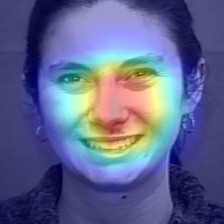
\includegraphics[width=\textwidth]{figures/models/gradcam_cnn+lstm_fold5/happy_pass.jpg}
		\caption{Happy}
	\end{subfigure}
	\begin{subfigure}{0.24\textwidth}
		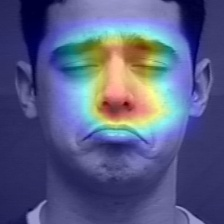
\includegraphics[width=\textwidth]{figures/models/gradcam_cnn+lstm_fold5/sad_pass.jpg}
		\caption{Sad (Corect)}
	\end{subfigure}
	\begin{subfigure}{0.24\textwidth}
		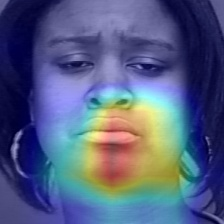
\includegraphics[width=\textwidth]{figures/models/gradcam_cnn+lstm_fold5/sad_FAIL_as_Anger.jpg}
		\caption{Sad $\to$ Anger}
	\end{subfigure}
	\begin{subfigure}{0.24\textwidth}
		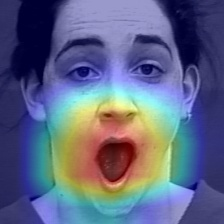
\includegraphics[width=\textwidth]{figures/models/gradcam_cnn+lstm_fold5/surprise_pass.jpg}
		\caption{Surprise}
	\end{subfigure}
	\caption{Vizualizarea regiunilor de interes prin Grad-CAM (Fold 5).}
	\label{fig:gradcam_grid}
\end{figure}

\subsubsection{Observații privind regiunile de interes}

Analiza hărților de activare a scos în evidență câteva aspecte contra-intuitive și interesante:

\begin{itemize}
	\item \textbf{Recunoașterea Fericirii (Happy):} Contrar așteptărilor, modelul nu se concentrează exclusiv pe zona gurii (zâmbet). Grad-CAM indică o activare intensă în \textbf{zona nasului} și a pliurilor nazolabiale. Acest lucru sugerează că modelul a învățat că lărgirea bazei nasului și ridicarea obrajilor sunt indicatori mai robuști pentru această clasă decât simpla deschidere a gurii.
	\item \textbf{Eroarea Sad vs. Anger:} În cazul eșantionului clasificat greșit, se observă că activarea Grad-CAM este localizată puternic între sprâncene. Modelul a interpretat contracția mușchiului \textit{corrugator supercilii} ca fiind specifică furiei, ignorând indiciile mai subtile de tristețe din jurul ochilor.
	\item \textbf{Surpriza:} Modelul prezintă o focalizare clară pe zona ochilor și a frunții, detectând ridicarea sprâncenelor, trăsătură anatomică definitorie pentru această emoție.
\end{itemize}

\section{Modelul ANN Echivalent: Izolarea Impactului Paradigmei de Spiking}

Pentru a determina în ce măsură performanța modelului bio-inspirat este influențată de arhitectura sa convoluțională versus mecanismul de spiking, a fost implementat un model \textbf{ANN Echivalent (Equivalent Baseline ANN)}. 

\subsection*{Arhitectură și Metodologie}
Acest model păstrează topologia hărților de trăsături ale CSNN-ului, dar înlocuiește neuronii de tip \textit{Leaky Integrate-and-Fire} cu unități de activare standard și învățare prin \textit{backpropagation}.

\begin{itemize}[noitemsep]
	\item \textbf{Configurație:} Strat convoluțional 3D (64 filtre, kernel $3 \times 5 \times 5$), urmat de \textit{Batch Normalization} și activare ReLU.
	\item \textbf{Pooling:} \texttt{AvgPool3d} ($2 \times 4 \times 4$), similar mecanismului de pooling din SNN.
	\item \textbf{Antrenare:} S-a utilizat optimizatorul Adam și funcția de cost \textit{Cross-Entropy}, fără augmentare de date, pentru a menține condițiile experimentale ale CSNN-ului.
	\item \textbf{Date de intrare:} S-au utilizat fețe pre-procesate (\textit{cropped}), eliminând fundalul pentru a permite modelului să conveargă rapid în absența augmentărilor.
\end{itemize}

\subsection*{Rezultate Experimentale}
Rezultatele pe cele 10 fold-uri sunt prezentate în Tabelul \ref{tab:rezultate_ann_echivalent}. Media obținută este de \textbf{73.23\%}, o valoare semnificativ superioară baseline-ului SVM, dar inferioară modelului complex CNN-LSTM.

\begin{table}[h!]
	\centering
	\caption{Performanța modelului ANN echivalent (3D Conv + ReLU)}
	\label{tab:rezultate_ann_echivalent}
	\begin{tabular}{lc|lc}
		\toprule
		\textbf{Fold} & \textbf{Acuratețe (\%)} & \textbf{Fold} & \textbf{Acuratețe (\%)} \\ \midrule
		Fold 1 & 75.76\% & Fold 6 & 67.86\% \\
		Fold 2 & 80.00\% & Fold 7 & 71.88\% \\
		Fold 3 & 72.73\% & Fold 8 & 65.52\% \\
		Fold 4 & 84.38\% & Fold 9 & 71.43\% \\
		Fold 5 & 69.70\% & Fold 10 & 73.08\% \\ \midrule
		\textbf{Medie} & \multicolumn{3}{c}{\textbf{73.23\%}} \\ \bottomrule
	\end{tabular}
\end{table}

\subsection*{Analiză Comparativă Finală}

Prezența acestui model în studiu permite o interpretare critică a rezultatelor:

\begin{enumerate}
	\item \textbf{Importanța Focalizării (Cropping):} Experimentele preliminare au arătat că utilizarea imaginilor complete (cu fundal) scade performanța ANN-ului la aproximativ 30-40\%. Acest lucru subliniază un avantaj teoretic al CSNN-ului: prin filtrarea On/Off și Latency Coding, SNN-ul este inherent mai robust la zgomotul de fundal (pixelii statici nu generează spike-uri), în timp ce un ANN clasic are nevoie de decuparea feței sau de volume masive de date pentru a ignora fundalul.
	\item \textbf{STDP vs. Backpropagation:} Diferența de la 48.02\% (SNN) la 73.23\% (ANN) reprezintă „costul” utilizării unei reguli de învățare locale și nesupervizate (STDP). Deși Backpropagation este mai precis, STDP oferă un avantaj major în termeni de eficiență energetică pe hardware neuromorfic și plauzibilitate biologică.
	\item \textbf{Concluzie:} Modelul ANN echivalent demonstrează că topologia 3D Conv este extrem de potrivită pentru setul CK+, dar eficiența implementării spike-based depinde critic de rafinarea mecanismelor de homeostazie și a pragurilor de activare.
\end{enumerate}

\chapter{Numele aplicației}

\chapter{Colectarea cerințelor}

În cadrul acestui capitol sunt detaliate funcționalitățile sistemului Neuro-Guardian, interacțiunile dintre utilizatori și platformă, precum și constrângerile tehnice sub care funcționează soluția propusă.

\section{Actorii sistemului}

Actorii reprezintă entitățile externe care interacționează cu sistemul. În cadrul platformei Neuro-Guardian, am identificat următoarele categorii:

\begin{itemize}
    \item \textbf{Angajat Spital:} Actorul generic care include funcționalitățile de bază de autentificare (Înregistrare, Autentificare, Deconectare).
    \item \textbf{Administrator:} Moștenește trăsăturile angajatului și are responsabilitatea gestionării fluxului administrativ al pacienților (internări, externări și alocarea resurselor/paturilor).
    \item \textbf{Doctor:} Actorul principal în procesul de îngrijire, responsabil de preluarea pacienților și monitorizarea stării lor clinice și emoționale în timp real.
    \item \textbf{Camera Web (Sistem Extern):} Furnizează fluxul de date video necesar procesului de captare a cadrelor.
    \item \textbf{CSNN - Convolutional Spiking Neural Network (Sistem Extern):} Modelul de inteligență artificială care procesează cadrele recepționate și returnează predicțiile emoționale.
\end{itemize}

\section{Diagrama cazurilor de utilizare}

Diagrama cazurilor de utilizare, prezentată în Figura \ref{fig:diagrama_uml}, oferă o imagine de ansamblu asupra modului în care funcționalitățile sunt distribuite între actori.

\begin{figure}[htbp]
    \centering
    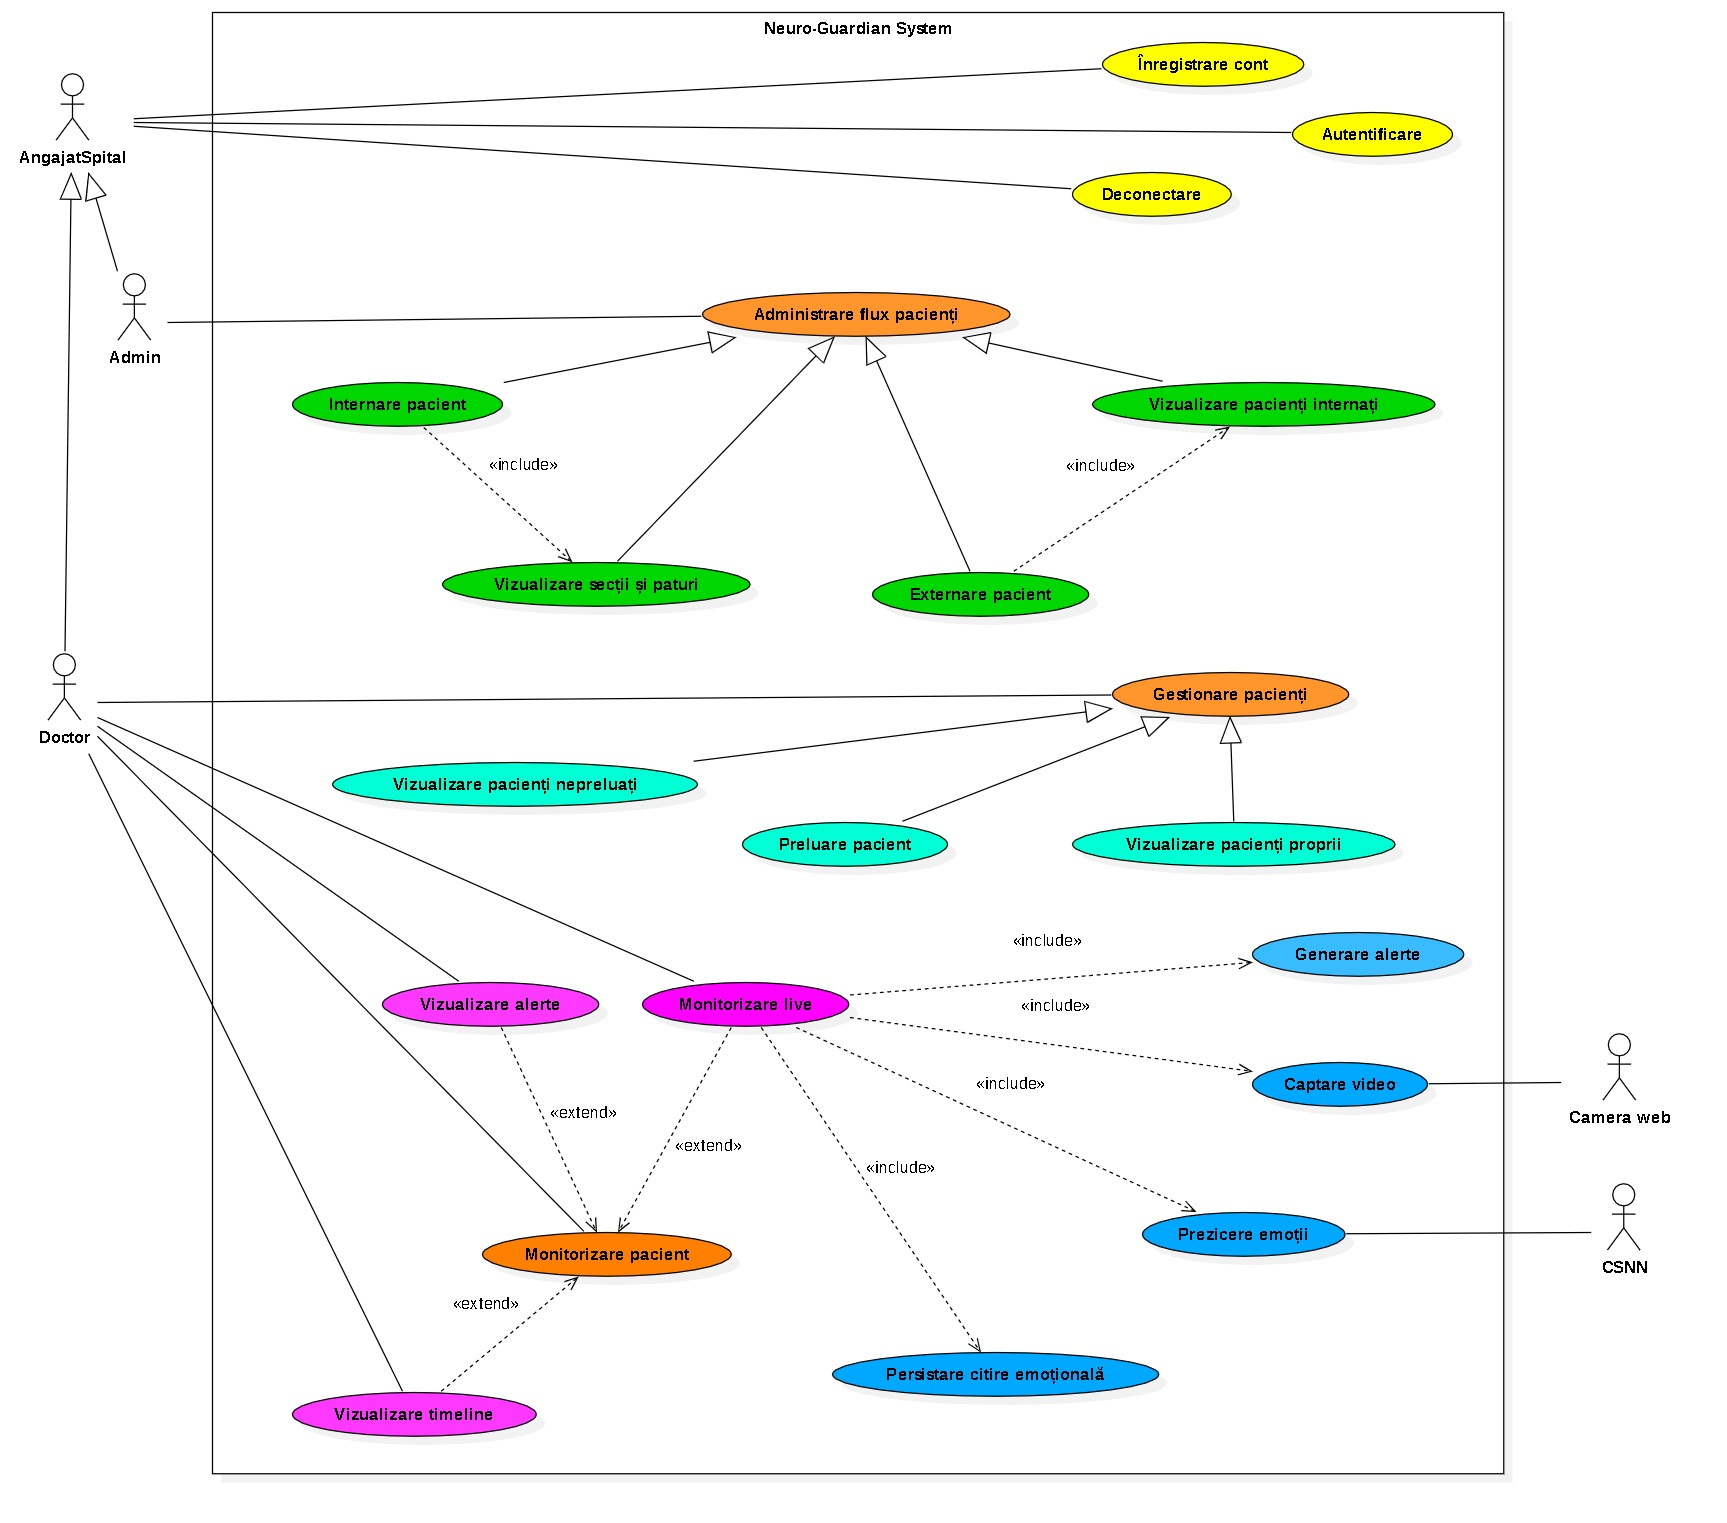
\includegraphics[width=0.83\textwidth]{figures/diagrams/UseCaseDiagram.jpg}
    \caption{Diagrama cazurilor de utilizare - Sistemul Neuro-Guardian}
    \label{fig:diagrama_uml}
\end{figure}

\section{Descrierea detaliată a unui caz de utilizare}

În această secțiune este detaliat fluxul principal de interacțiune pentru cazul de utilizare \textbf{Gestionare Pacienți}, reprezentat grafic în Figura \ref{fig:diagrama_uml}. Acest caz de utilizare este central pentru activitatea clinică a medicului, asigurând tranziția între selecția pacienților și monitorizarea activă.

\begin{table}[htbp]
\centering
\small
\begin{tabularx}{\textwidth}{|l|X|}
\hline
\rowcolor[HTML]{EFEFEF} 
\multicolumn{2}{|l|}{\textbf{Elemente de identificare}} \\ \hline
\textbf{Nume} & Gestionare pacienți \\ \hline
\textbf{Actori} & Doctor \\ \hline
\textbf{Descriere} & Procesul prin care un medic vizualizează lista pacienților din secție, preia responsabilitatea pentru un pacient nou sau comută între pacienții deja asignați pentru a vizualiza datele biometrice și emoționale. \\ \hline

\rowcolor[HTML]{EFEFEF} 
\multicolumn{2}{|l|}{\textbf{Condiții de context}} \\ \hline
\textbf{Precondiții} & 1. Medicul este autentificat în sistem. \newline 2. Pacienții sunt deja internați în secție (via Admin). \newline 3. Conexiunea WebSocket cu modelul AI este activă. \\ \hline
\textbf{Postcondiții} & Interfața reflectă starea în timp real a pacientului selectat, iar baza de date actualizează relația medic-pacient. \\ \hline

\rowcolor[HTML]{EFEFEF} 
\multicolumn{2}{|l|}{\textbf{Scenariu Principal de Succes (MSS)}} \\ \hline
\textbf{Flux normal} & 
1. Medicul accesează dashboard-ul; sistemul afișează implicit datele ultimului pacient preluat. \newline
2. Medicul acționează butonul „Show panel” pentru a extinde panoul de selecție. \newline
3. Sistemul interoghează baza de date și afișează două liste: „Available Patients” și „My Patients”. \newline
4. Medicul identifică un pacient nepreluat și selectează opțiunea „Take patient”. \newline
5. Sistemul realizează maparea medic-pacient și trimite medicul către pagina destinată pacientului respectiv\newline
6. Medicul selectează un alt pacient din lista „My Patients” pentru a verifica evoluția acestuia. \newline
7. Sistemul comută contextul de monitorizare, afișând informațiile specifice noului pacient selectat. \newline
8. Medicul acționează „Hide panel” pentru a maximiza spațiul de vizualizare a detaliilor pacientului. \newline
9. Sistemul ascunde panoul lateral și trece în modul de monitorizare imersivă. \\ \hline

\rowcolor[HTML]{EFEFEF} 
\multicolumn{2}{|l|}{\textbf{Scenarii alternative}} \\ \hline
\textbf{Alt. 1} & \textbf{Medicul nu are pacienți în responsabilitate:} \newline
1a. Sistemul afișează un mesaj de informare și prezintă doar lista pacienților nepreluați. \newline
1b. Medicul efectuează preluarea primului pacient (se revine la pasul 5 din MSS). \\ \hline
\textbf{Alt. 2} & \textbf{Inexistența pacienților nepreluați:} \newline
3a. Lista „Available patients” apare goală; medicul poate gestiona doar portofoliul actual de pacienți (se revine la pasul 6 din MSS). \\ \hline

\rowcolor[HTML]{EFEFEF} 
\multicolumn{1}{|l|}{\textbf{Excepții}} \\ \hline
\textbf{Excepție 1} & \textbf{Pacientul este externat simultan:} Sistemul blochează preluarea și notifică medicul că datele nu mai sunt disponibile. \\ \hline

\rowcolor[HTML]{EFEFEF} 
\multicolumn{2}{|l|}{\textbf{Cerințe de calitate}} \\ \hline
\textbf{Performanță} & Timpul de comutare între doi pacienți nu trebuie să depășească 1 secundă pentru datele textuale. \\ \hline
\textbf{Fiabilitate} & Persistarea asocierii medic-pacient trebuie să fie confirmată tranzacțional în baza de date. \\ \hline
\end{tabularx}
\caption{Descrierea detaliată a scenariului de utilizare: Gestionare pacienți}
\label{tab:detaliu_gestiune}
\end{table}

\section{Cerințe nefuncționale (NFR)}

Cerințele nefuncționale definesc criteriile de calitate și constrângerile tehnice ale sistemului.

\subsection{Securitate și control acces}
\begin{itemize}
    \item \textbf{NFR-S1:} Toate operațiile sensibile necesită autentificare pe bază de Bearer JWT.
    \item \textbf{NFR-S2:} Autorizare strictă pe rol (ADMIN vs DOCTOR); medicii pot vizualiza doar pacienții care le sunt asignați.
    \item \textbf{NFR-S3:} Parolele sunt stocate exclusiv în format hashed folosind algoritmul \textit{bcrypt}.
    \item \textbf{NFR-S4:} Token-urile au timp de expirare implementat, iar refresh token-urile sunt rotite automat și invalidate la logout.
    \item \textbf{NFR-S5:} Validarea riguroasă a input-ului la frontierele API (câmpuri obligatorii, formate de timestamp valide).
\end{itemize}

\subsection{Confidențialitate și protecția datelor}
\begin{itemize}
    \item \textbf{NFR-P1:} Datele pacienților sunt accesibile doar personalului medical autorizat direct.
    \item \textbf{NFR-P2:} Minimizarea expunerii datelor; sistemul nu afișează informații care nu sunt necesare contextului clinic curent.
    \item \textbf{NFR-P3:} Comunicația între client și server se realizează prin protocoale criptate HTTPS/WSS (TLS).
\end{itemize}

\subsection{Performanță și timp real}
\begin{itemize}
    \item \textbf{NFR-F1:} Afișarea emoțiilor se realizează aproape în timp real prin WebSocket, cu o latență minimă, în timp ce persistarea în baza de date se face periodic.
    \item \textbf{NFR-F2:} Limitarea backlog-ului de cadre video procesate pentru a preveni consumul excesiv de memorie RAM pe client.
    \item \textbf{NFR-F3:} Dashboard-ul rămâne responsiv și funcțional chiar și în perioadele de indisponibilitate a motorului de analiză AI.
\end{itemize}

\subsection{Fiabilitate și disponibilitate}
\begin{itemize}
    \item \textbf{NFR-R1:} Mecanism de \textit{fallback}: dacă InfluxDB este indisponibil, sistemul utilizează baza de date principală (Postgres) sau date sintetice pentru continuitate.
    \item \textbf{NFR-R2:} Interfața semnalează vizual deconectarea modelului AI, permițând utilizatorului să continue alte activități administrative.
    \item \textbf{NFR-R3:} Operațiile critice (Check-in/Check-out) sunt tratate tranzacțional pentru a menține consistența între starea patului și cea a pacientului.
\end{itemize}

\subsection{Uzabilitate și Mentenabilitate}
\begin{itemize}
    \item \textbf{NFR-U1:} Interfața oferă feedback vizual clar pentru stările de încărcare sau eroare (Loading/Error states).
    \item \textbf{NFR-M1:} Arhitectură modulară bazată pe TypeScript, cu separare clară între controller, rute și servicii.
    \item \textbf{NFR-M3:} Aplicația este cross-platform (Windows/Linux) utilizând stack-ul Node.js și Vite.
\end{itemize}

\section{Modelul structural}
\label{sec:model-structural}

\subsection{Backend}
\label{subsec:model-structural-backend}

\begin{figure}[htbp]
  \centering

  \begin{subfigure}[t]{0.99\textwidth}
    \centering
    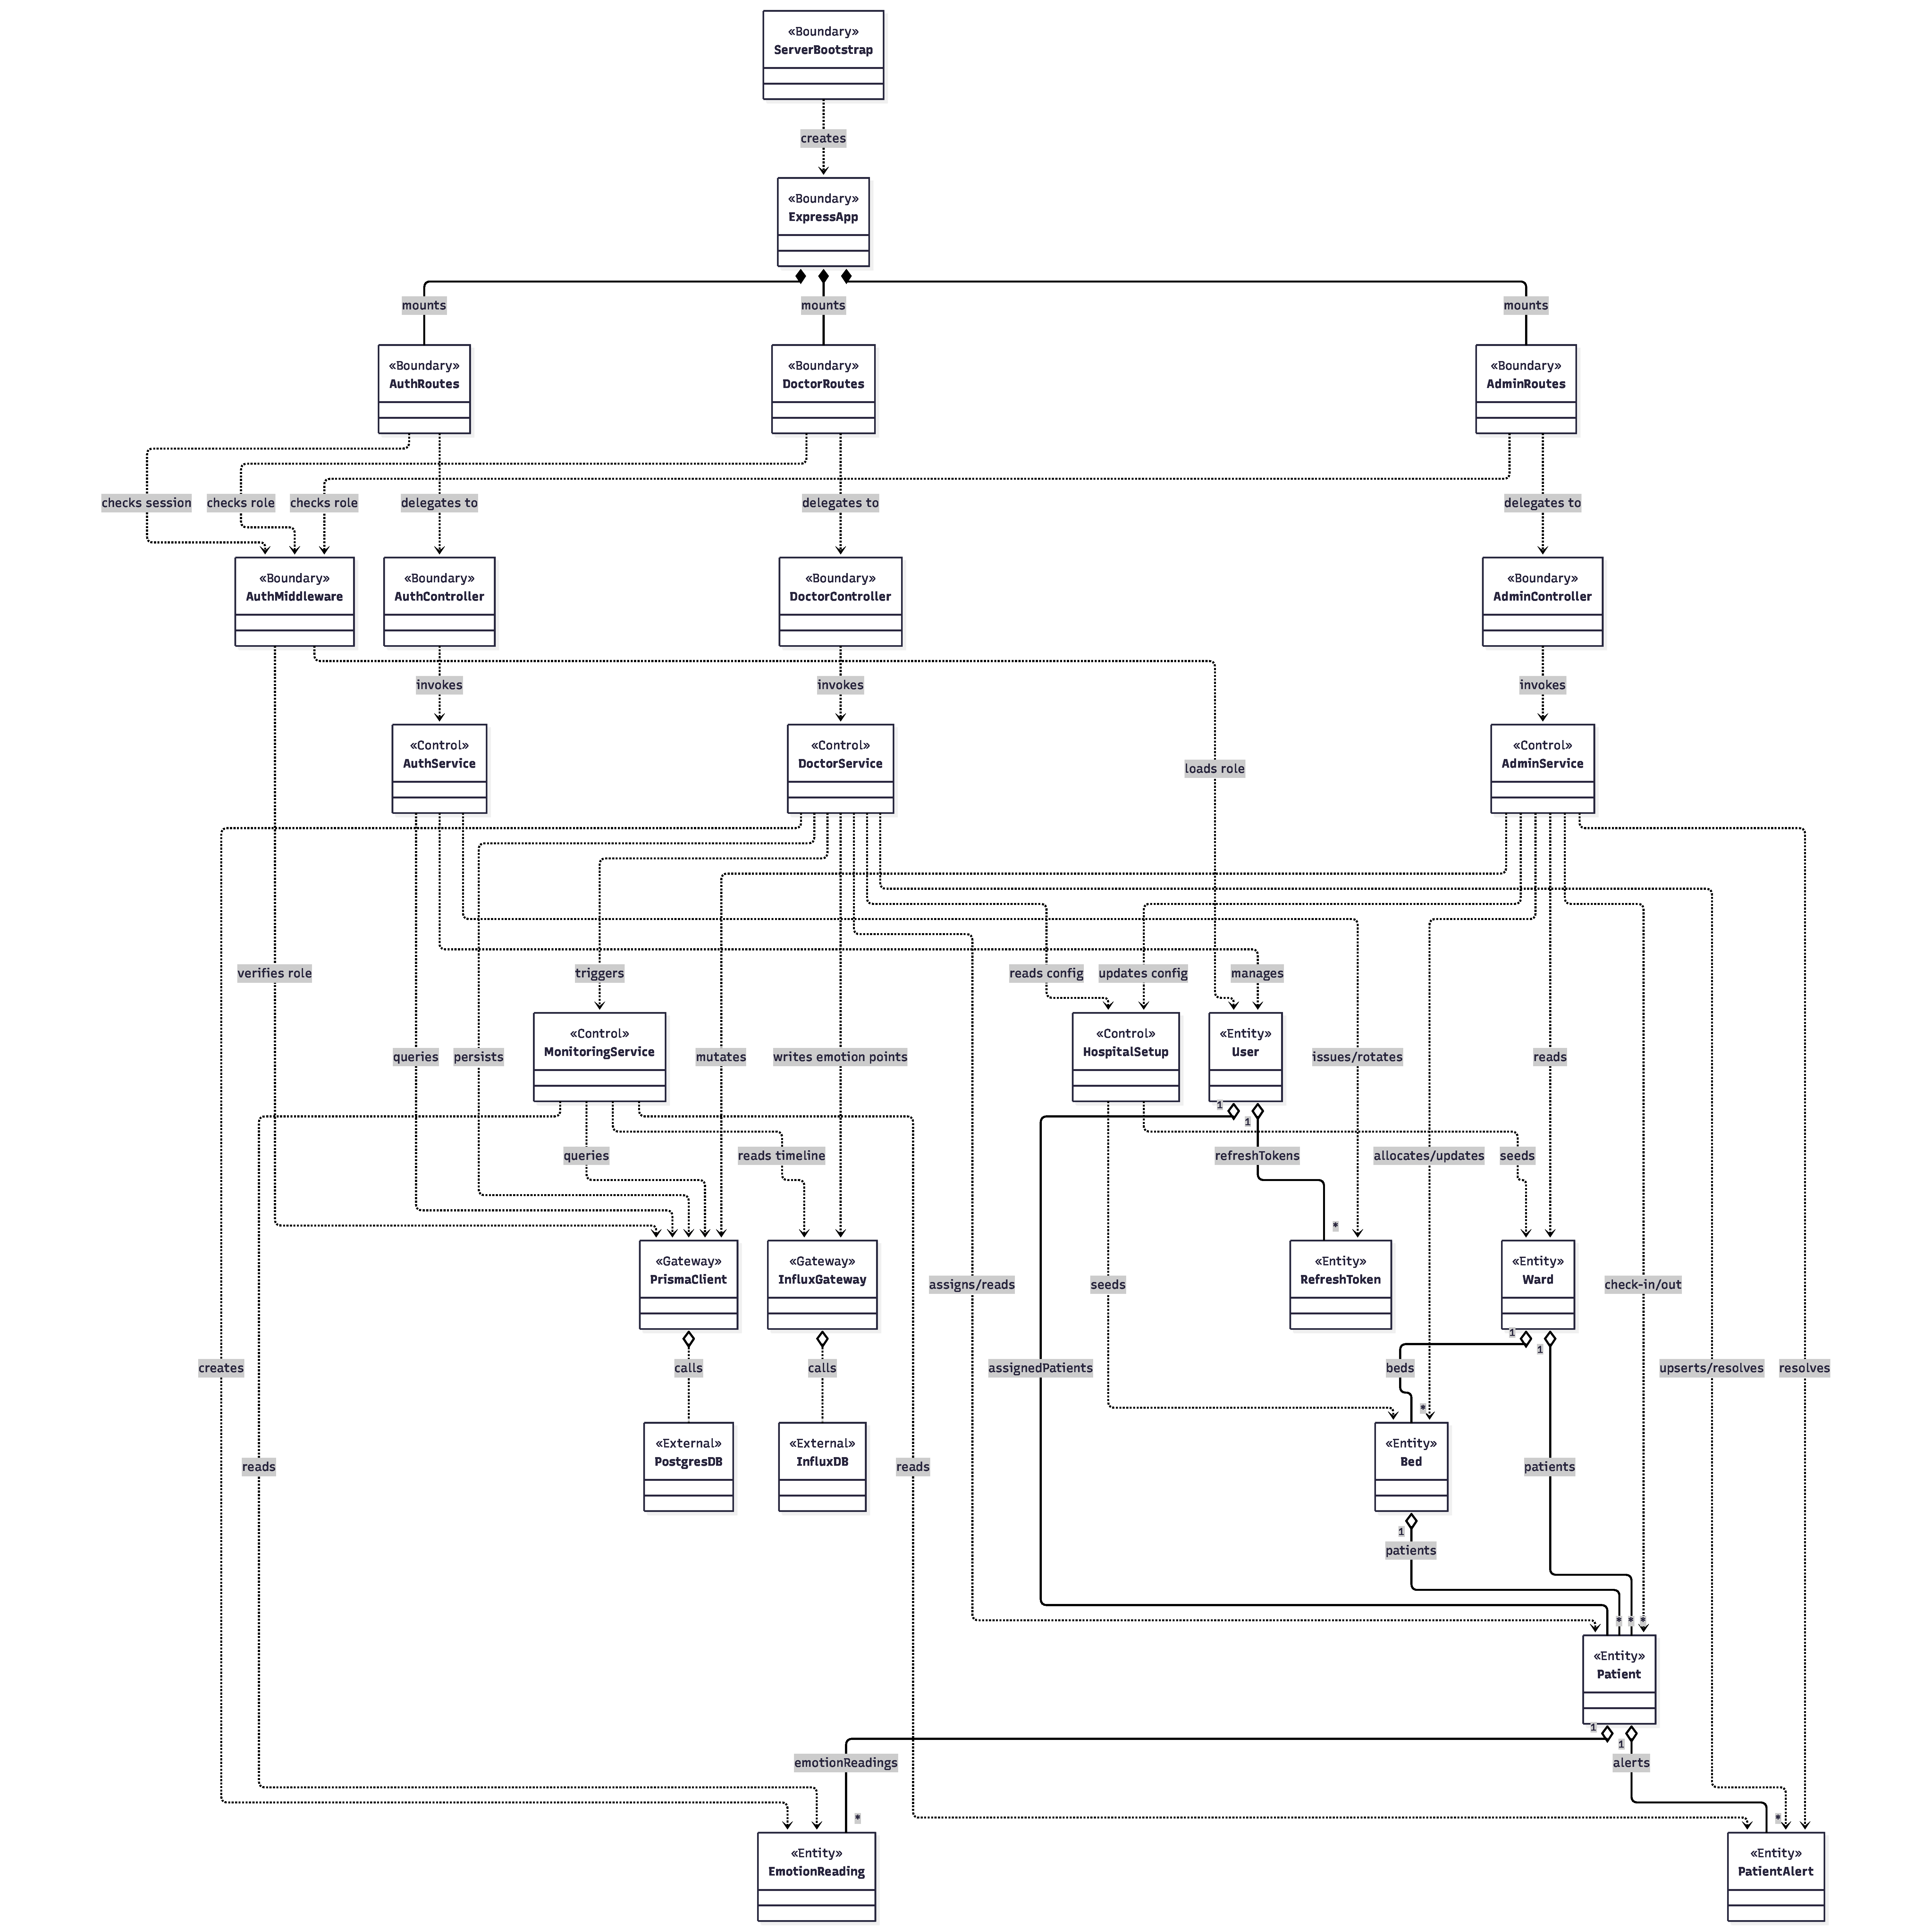
\includegraphics[width=\textwidth]{figures/diagrams/backend-class-diagram-1.pdf}
    \caption{API-ul HTTP: Boundary (Express/Routes/Controllers/Middleware), Control (Services) și persistența prin Gateway/External.}
    \label{fig:backend-ecb-api}
  \end{subfigure}

  \vspace{0.6em}

  \begin{subfigure}[t]{0.99\textwidth}
    \centering
    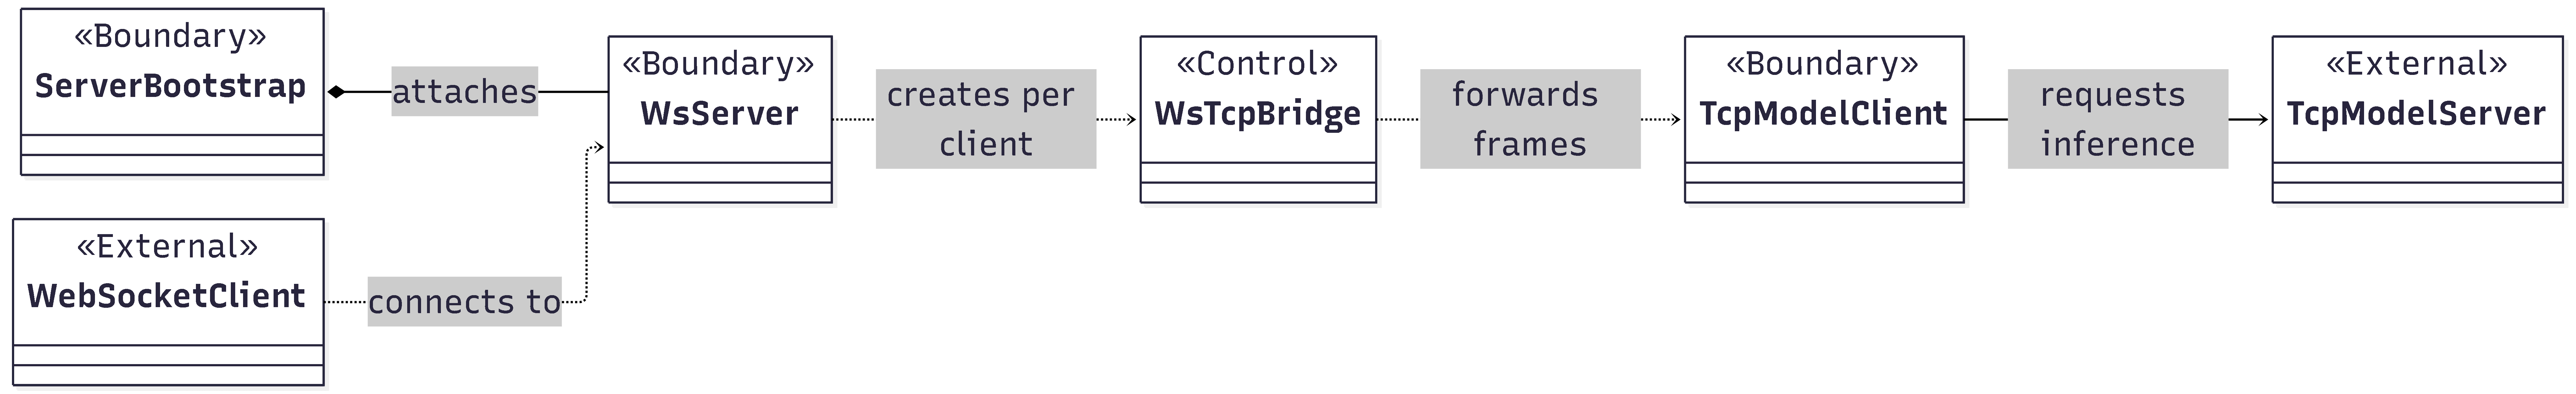
\includegraphics[width=\textwidth]{figures/diagrams/backend-class-diagram-2.png}
    \caption{Canalul de inferență în timp real: WebSocket \texorpdfstring{$\leftrightarrow$}{<->} TCP (model extern).}
    \label{fig:backend-ecb-stream}
  \end{subfigure}

  \caption{Modelul structural al backend-ului, conform ECB (Entity--Control--Boundary) extins cu Gateway și External.}
  \label{fig:backend-ecb}
\end{figure}

Figura~\ref{fig:backend-ecb-api} și Figura~\ref{fig:backend-ecb-stream} ilustrează organizarea backend-ului bazată pe modelul arhitectural \textit{Entity--Control--Boundary} (ECB), structură care asigură o separare clară a responsabilităților:
\begin{itemize}
  \item \textit{Entity} reprezintă nucleul domeniului, adică modelele persistente gestionate în baza de date (ex.: \textit{User}, \textit{Patient}, \textit{EmotionReading}, \textit{PatientAlert}).
  \item \textit{Control} concentrează logica de business și orchestrează fluxurile de lucru (serviciile aplicației).
  \item \textit{Boundary} delimitează interfața către exterior și gestionează comunicarea cu clienții (rute, controllere, middleware, servere de transport).
\end{itemize}

Pentru integrarea cu infrastructura, arhitectura este extinsă cu etichetele \textit{Gateway} și \textit{External}, care izolează accesul la servicii externe și decuplează logica internă de detaliile tehnice (de exemplu, accesul la baze de date). În Figura~\ref{fig:backend-ecb-api}, inițializarea aplicației este realizată de \textit{ServerBootstrap} și \textit{ExpressApp}, care montează rutele (\textit{AuthRoutes}, \textit{DoctorRoutes}, \textit{AdminRoutes}) și aplică \textit{AuthMiddleware} pentru validarea sesiunii și a rolurilor. La nivelul stratului de expunere HTTP, componentele de tip controller (AuthController, DoctorController, AdminController) au fost proiectate conform paradigmei de 'thin controllers' (asigurând o logică minimală de procesare) și deleagă operațiile către servicii (\textit{AuthService}, \textit{DoctorService}, \textit{AdminService}), astfel încât regulile de business și validările specifice domeniului să fie centralizate și ușor de întreținut. Serviciile operează asupra entităților domeniului (de exemplu, \textit{AuthService} gestionează \textit{User}/\textit{RefreshToken}, \textit{DoctorService} gestionează \textit{Patient}/\textit{EmotionReading}/\textit{PatientAlert}, iar \textit{AdminService} gestionează \textit{Ward}/\textit{Bed}/\textit{Patient}).

Persistența și integrarea sunt decuplate prin gateway-uri: \textit{PrismaClient} mediază accesul la baza de date relațională (PostgreSQL), iar \textit{InfluxGateway} asigură scrierea/citirea seriilor temporale în InfluxDB, pentru vizualizări și analiză istorică. Separat de fluxul HTTP, Figura~\ref{fig:backend-ecb-stream} prezintă canalul de procesare în timp real pentru inferență: \textit{WsServer} acceptă conexiuni de la clientul WebSocket al aplicației web, iar \textit{WsTcpBridge} orchestrează fluxul dintre WebSocket și modelul extern, trimițând frame-urile prin \textit{TcpModelClient} către \textit{TcpModelServer}. Rezultatele inferenței (probabilități) sunt retransmise către client, păstrând responsabilitățile de transport separate de logica de business și de mecanismele de stocare.

\subsection{Frontend}
\label{subsec:model-structural-frontend}

% Necesită \usepackage{subcaption} în preambul (pentru subfigure).

\begin{figure}[htbp]
  \centering

  \begin{subfigure}[t]{0.7\textwidth}
    \centering
    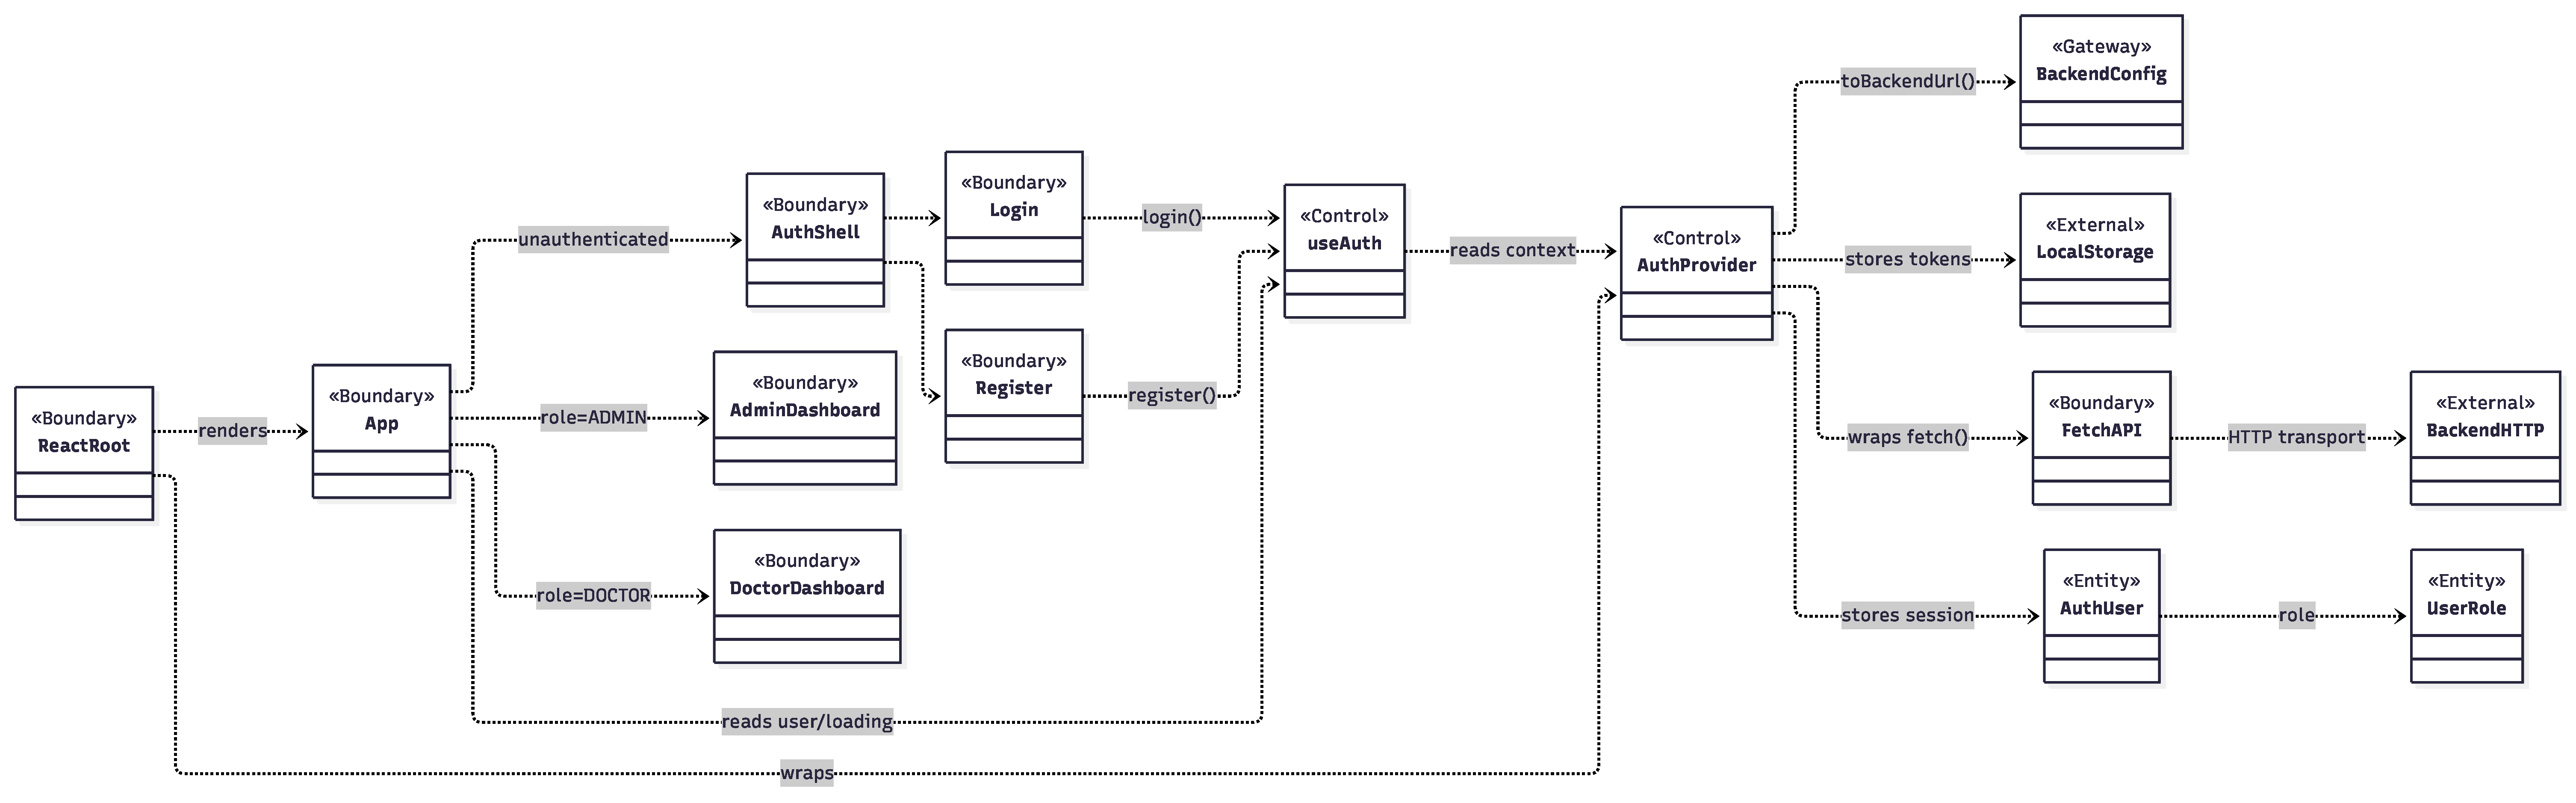
\includegraphics[width=\textwidth]{figures/diagrams/frontend-class-diagram-1.pdf}
    \caption{Bootstrap și autentificare (App Shell).}
    \label{fig:frontend-ecb-auth}
  \end{subfigure}

  \vspace{0.6em}

  \begin{subfigure}[t]{0.7\textwidth}
    \centering
    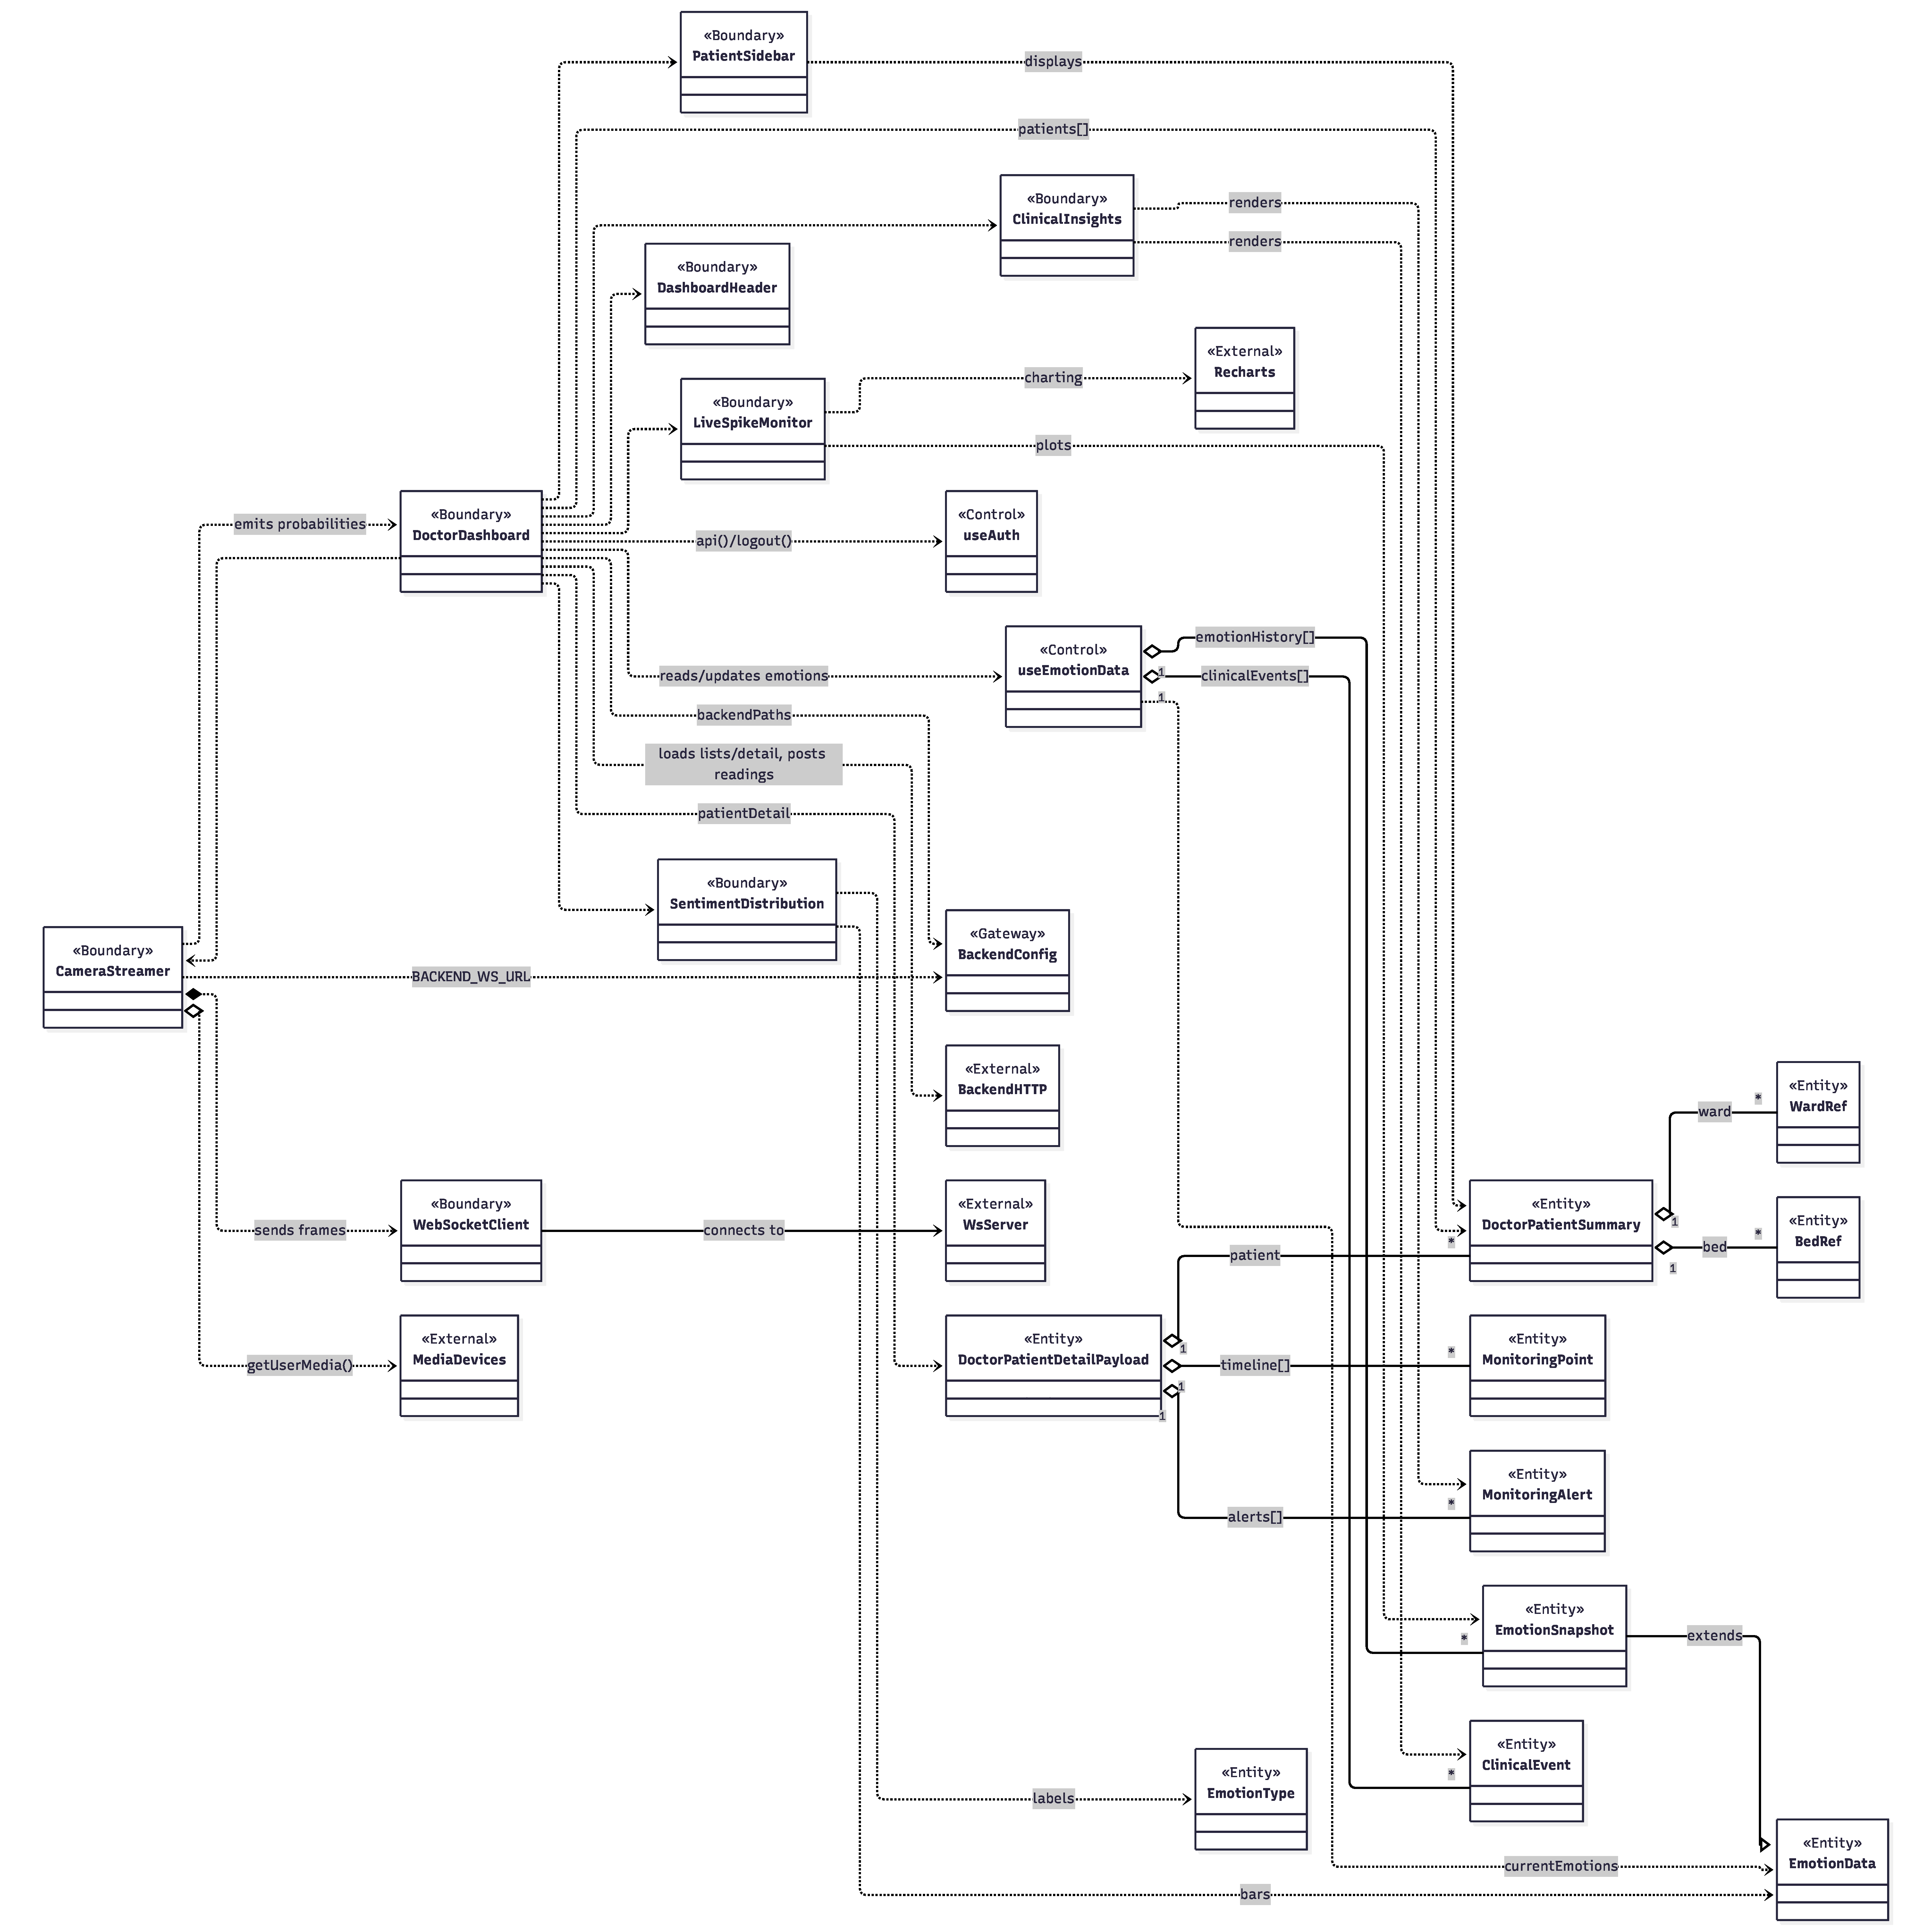
\includegraphics[width=\textwidth]{figures/diagrams/frontend-class-diagram-2.pdf}
    \caption{Fluxul medicului: monitorizare, vizualizare și streaming live.}
    \label{fig:frontend-ecb-doctor}
  \end{subfigure}

  \vspace{0.6em}

  \begin{subfigure}[t]{0.65\textwidth}
    \centering
    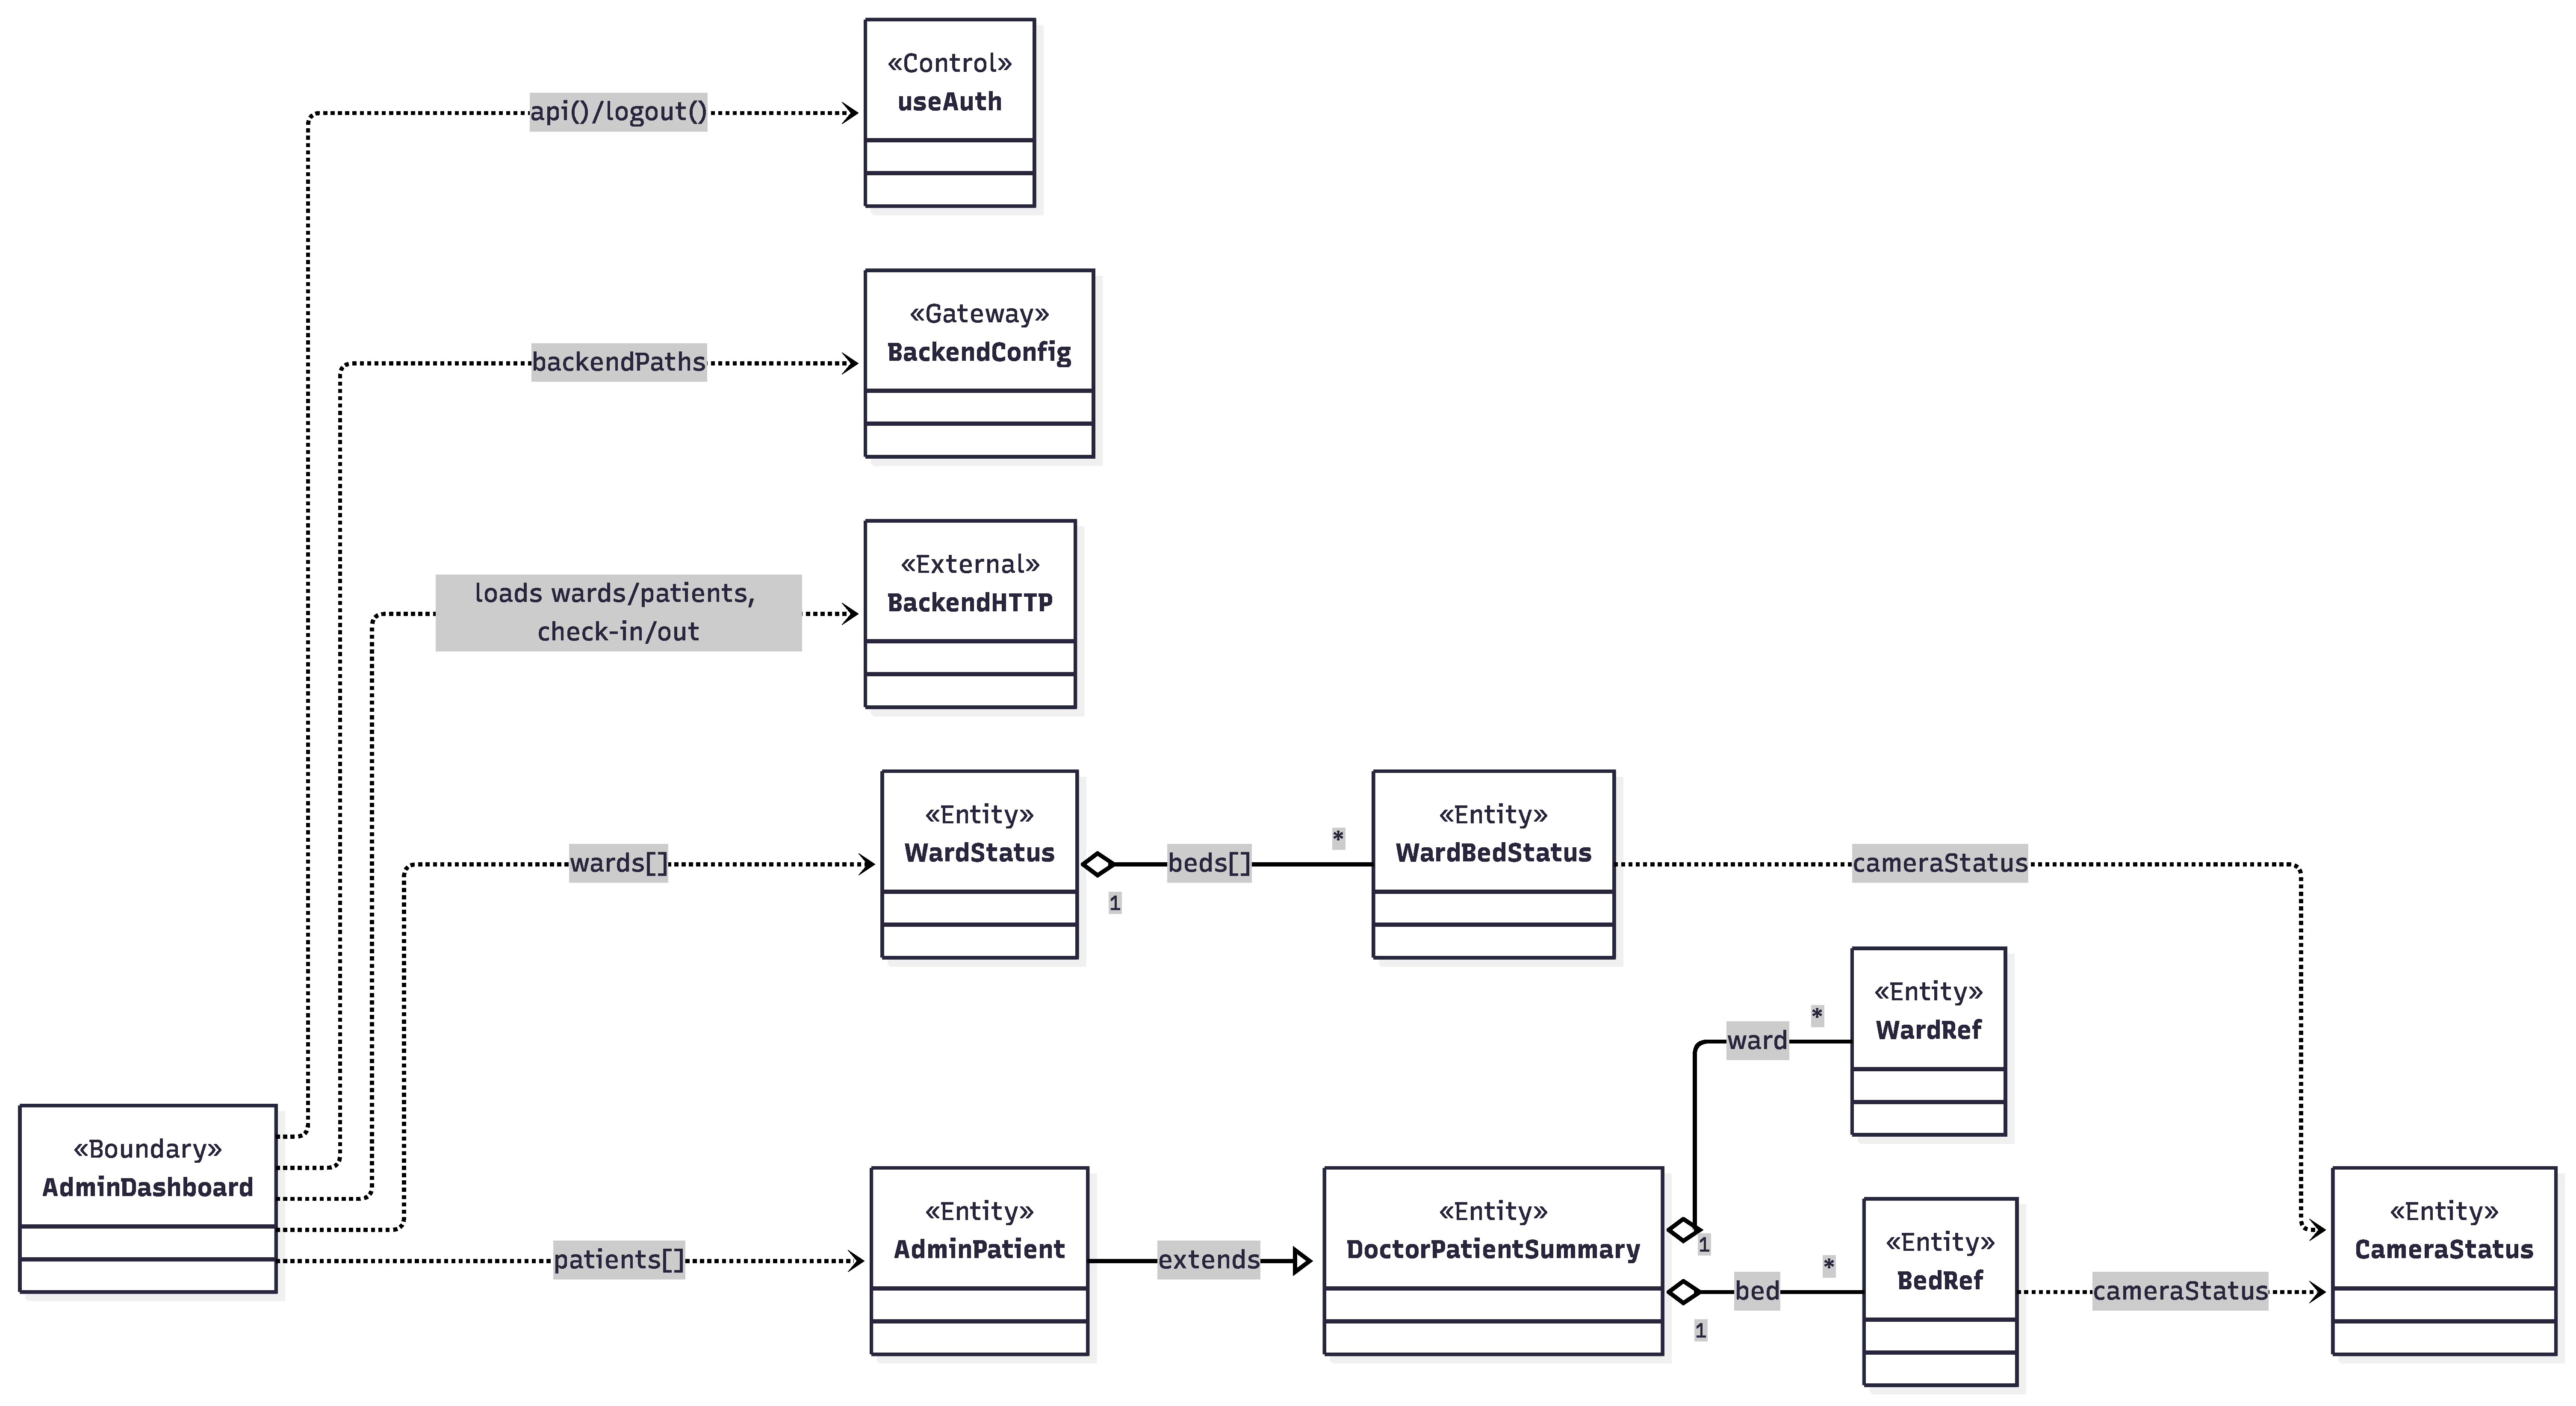
\includegraphics[width=\textwidth]{figures/diagrams/frontend-class-diagram-3.pdf}
    \caption{Fluxul administrativ: management secții/paturi/pacienți.}
    \label{fig:frontend-ecb-admin}
  \end{subfigure}

  \caption{Modelul structural al frontend-ului, conform ECB (Entity--Control--Boundary), extins cu Gateway și External.}
  \label{fig:frontend-ecb}
\end{figure}

Figura~\ref{fig:frontend-ecb} prezintă structura frontend-ului (React + TypeScript) folosind aceeași separare ECB ca în backend, însă cu o nuanță importantă: \textit{Entity} reprezintă în principal \textbf{modele de date/DTO-uri și stări UI} (de ex. \textit{AuthUser}, \textit{DoctorPatientSummary}, \textit{MonitoringPoint}), nu entități persistate direct în aplicația client. \textit{Control} grupează logica de orchestrare (hook-uri precum \textit{useAuth}, \textit{useEmotionData} și provider-ul \textit{AuthProvider}), iar \textit{Boundary} include paginile și componentele UI (de ex. \textit{App}, \textit{DoctorDashboard}, \textit{CameraStreamer}, \textit{LiveSpikeMonitor}). Pentru integrare, sunt evidențiate și componente \textit{Gateway}/\textit{External}, care izolează accesul la resurse de infrastructură (configurația către backend, transport HTTP/WS, API-uri ale browserului).

În Figura~\ref{fig:frontend-ecb-auth} este surprinsă fundația aplicației: \textit{ReactRoot} compune \textit{AuthProvider} peste \textit{App}, iar aplicația decide ruta principală în funcție de sesiune și rol. \textit{AuthProvider} centralizează autentificarea și persistă token-urile în \textit{LocalStorage}, oferind un API unificat pentru cereri HTTP (prin \textit{FetchAPI} și configurarea adreselor prin \textit{BackendConfig}). Această separare reduce duplicarea și menține componentele de UI independente de detaliile de transport.

Figura~\ref{fig:frontend-ecb-doctor} descrie fluxul principal al medicului: \textit{DoctorDashboard} încarcă lista de pacienți și detaliile de monitorizare din backend (DTO-uri precum \textit{DoctorPatientDetailPayload}, \textit{MonitoringPoint}, \textit{MonitoringAlert}), apoi compune componente specializate pentru vizualizare și suport decizional. Starea „live” a sesiunii este gestionată de \textit{useEmotionData} (entități UI precum \textit{EmotionData}, \textit{EmotionSnapshot}, \textit{ClinicalEvent}), în timp ce \textit{CameraStreamer} folosește \textit{MediaDevices} pentru captură și un \textit{WebSocketClient} dedicat pentru trimiterea frame-urilor către backend. Probabilitățile primite sunt propagate către dashboard pentru actualizarea UI și, periodic, pentru persistență prin endpoint-urile HTTP (ex. trimiterea de readings).

În Figura~\ref{fig:frontend-ecb-admin} este reprezentat fluxul administrativ, unde \textit{AdminDashboard} gestionează operațiile de check-in/check-out și statusul secțiilor/paturilor folosind DTO-uri precum \textit{WardStatus}, \textit{WardBedStatus} și \textit{AdminPatient}. Ca și în cazul medicului, comunicarea cu backend-ul este abstractizată prin \textit{useAuth} și aceeași infrastructură de transport/configurare, menținând UI-ul concentrat pe logică de prezentare și pe interacțiunile specifice rolului.

\subsection{Diagrama entitate--relație (ER)}
\label{subsec:model-structural-er}

\begin{figure}[htbp]
  \centering
  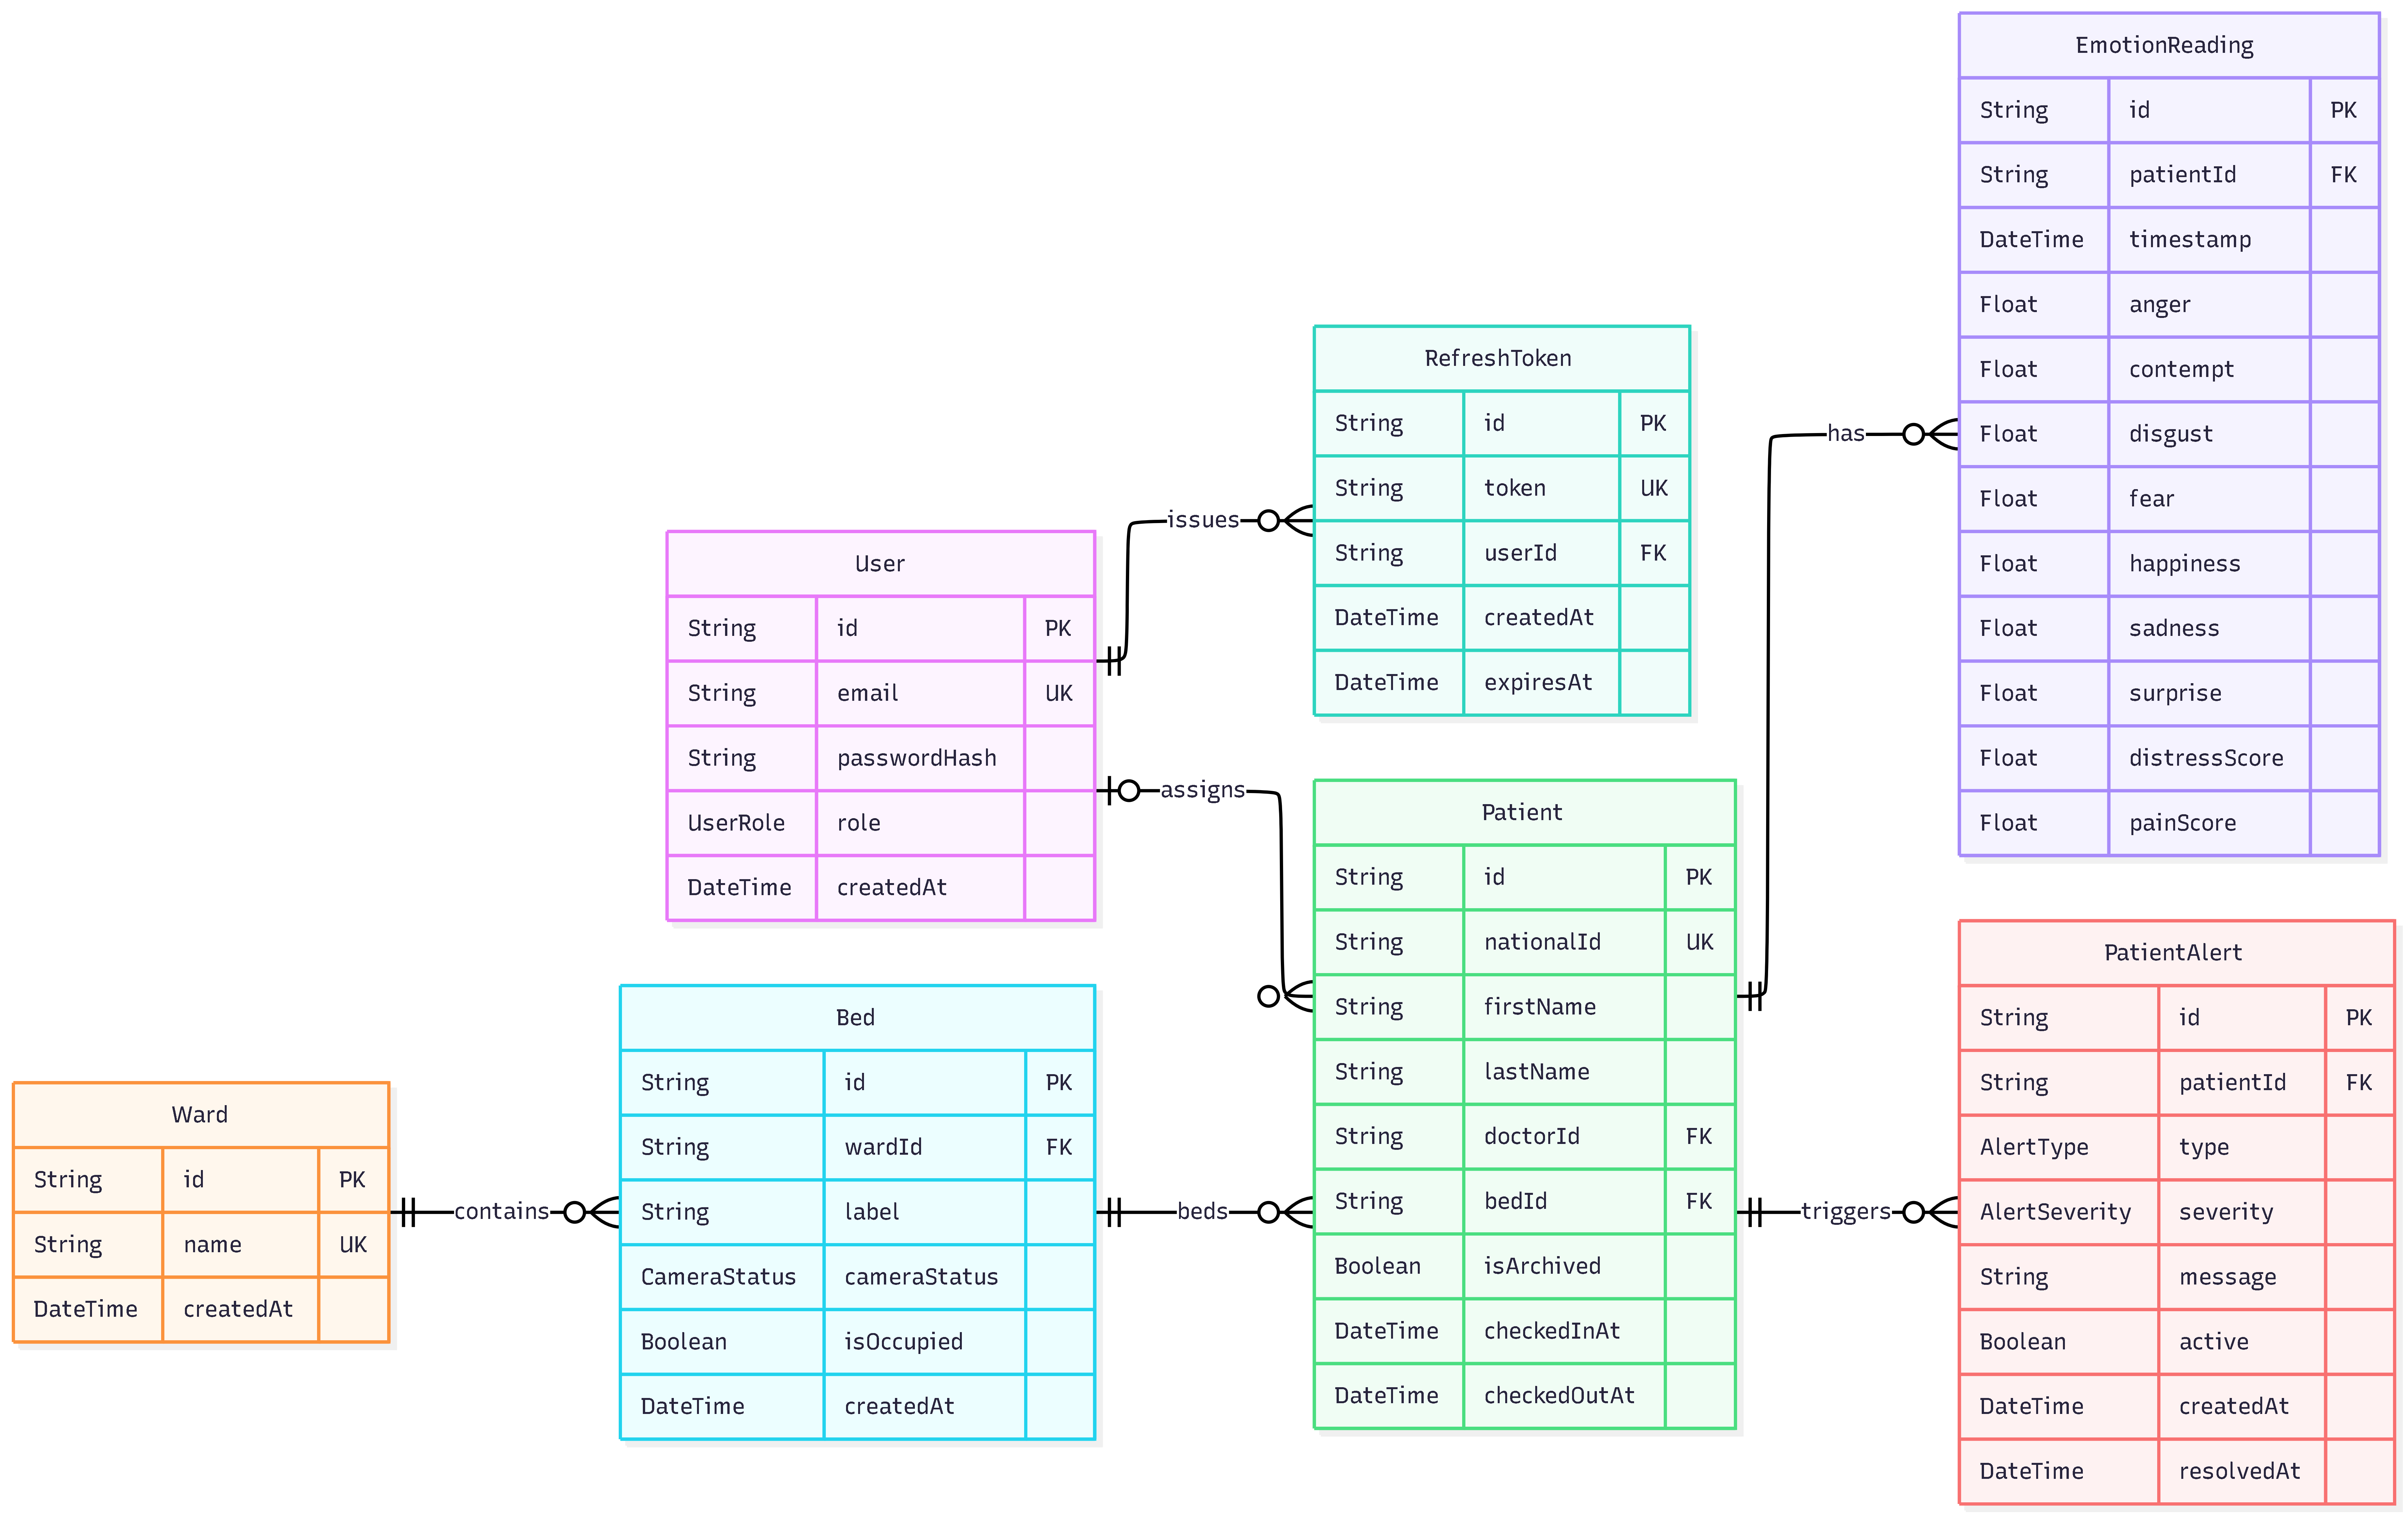
\includegraphics[width=0.9\textwidth]{figures/diagrams/entity_relationship_diagram.png}
  \caption{Diagrama entitate--relație (ER) a bazei de date.}
  \label{fig:backend-er}
\end{figure}

Figura~\ref{fig:backend-er} prezintă modelul relațional al datelor persistente utilizate de aplicație, complementând diagramele ECB. Dacă în modelul structural \textit{Entity} apare ca „nucleu al domeniului”, diagrama ER detaliază modul în care acest nucleu este implementat în baza de date: chei primare, chei străine, constrângeri de unicitate și relațiile dintre entități (cardinalități).

Zona de autentificare este compusă din \textit{User} și \textit{RefreshToken}: fiecare utilizator poate emite mai multe refresh token-uri (relația \textit{User}--\textit{RefreshToken}), iar câmpul \textit{role} (\textit{UserRole}) diferențiază fluxurile și permisiunile din aplicație (medic vs. administrator). La nivel operațional, aceste entități susțin sesiuni persistente și controlul accesului pe roluri.

Modelarea spitalului și a monitorizării este structurată în jurul entității \textit{Patient}, care este asociată cu o secție (\textit{Ward}) și un pat (\textit{Bed}), iar opțional poate fi asignată unui medic (\textit{User}). Starea clinică în timp este capturată prin \textit{EmotionReading} (seturi de valori pe emoții + scoruri agregate), legate de pacient, iar evenimentele de risc sunt reprezentate prin \textit{PatientAlert} (tip, severitate, activ/rezolvat). În acest fel, baza de date relațională păstrează atât structura organizațională (secții/paturi/pacienți), cât și istoricul și semnalările necesare fluxurilor din interfața medicului și a administratorului.

\section{Modelul dinamic al sistemului}
\label{sec:model-dinamic}

\subsection{Diagrama de secvență: Monitorizare live}
\label{subsec:model-dinamic-secventa-live}

\begin{figure}[htbp]
  \centering
  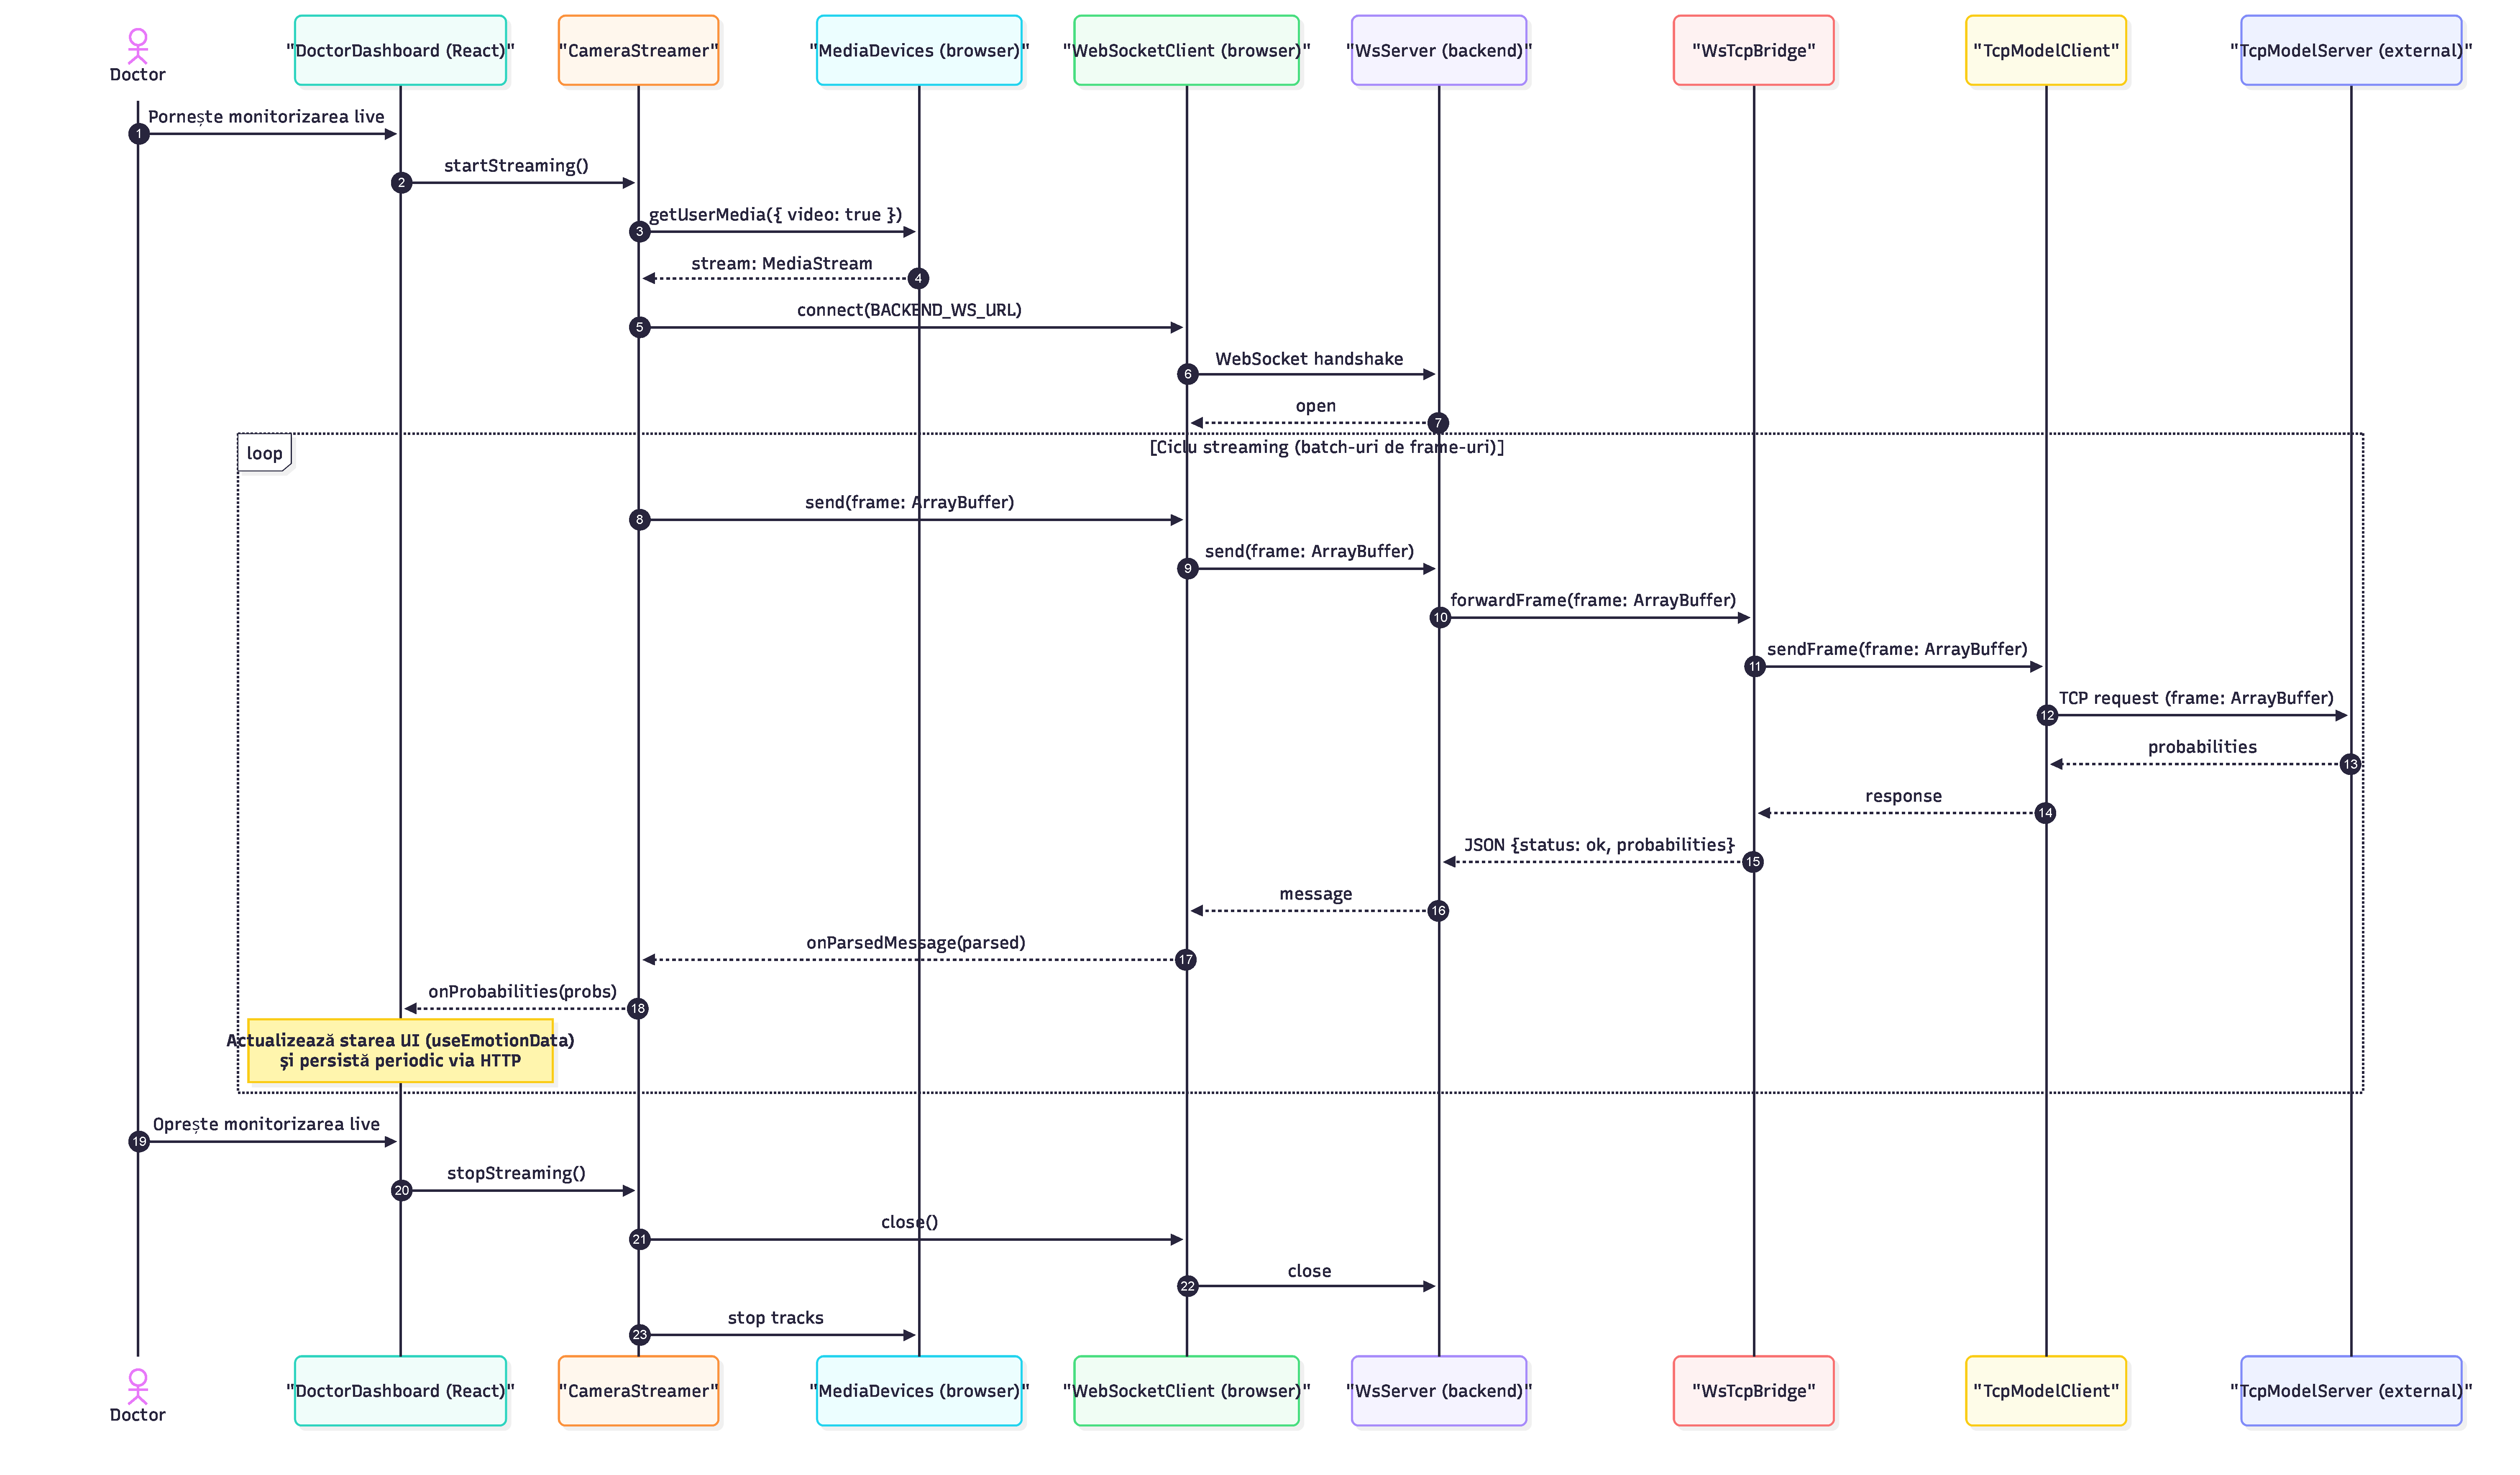
\includegraphics[width=0.99\textwidth]{figures/diagrams/diagrama-SD.pdf}
  \caption{Diagrama de secvență pentru use case-ul \textit{Monitorizare live}: captură video, transmitere prin WebSocket și inferență în model extern (TCP).}
  \label{fig:seq-monitor-live}
\end{figure}

Figura~\ref{fig:seq-monitor-live} descrie fluxul de monitorizare în timp real, declanșat de medic din interfața aplicației. La pornirea sesiunii, componenta de captură inițializează camera folosind API-ul browserului (\textit{MediaDevices}) și stabilește o conexiune WebSocket către backend. Cadrele video sunt pre-procesate (redimensionare/compresie) și transmise ca mesaje binare către server, permițând un canal cu latență redusă față de un flux exclusiv HTTP.

Pe backend, serverul WebSocket primește cadrele și le direcționează către un modul de tip „bridge” care gestionează ordonarea și trimiterea lor către modelul extern. Bridge-ul asigură conectarea către serviciul de inferență (prin clientul TCP) și aplică un mecanism de coadă, astfel încât procesarea să rămână stabilă chiar și când rata de captură depășește temporar capacitatea modelului. Rezultatul inferenței (probabilități pe emoții) este apoi serializat și retransmis prin WebSocket către aplicația web.

La nivel de UI, probabilitățile primite sunt folosite pentru actualizarea stării de monitorizare (grafice, distribuții, evenimente clinice) fără a bloca interacțiunea utilizatorului. Oprirea monitorizării închide conexiunea WebSocket și eliberează resursele de captură (oprirea track-urilor camerei), închizând complet bucla de streaming.

\subsection{Diagrama de comunicare: Vizualizare timeline}
\label{subsec:model-dinamic-comunicare-timeline}

\begin{figure}[htbp]
  \centering
  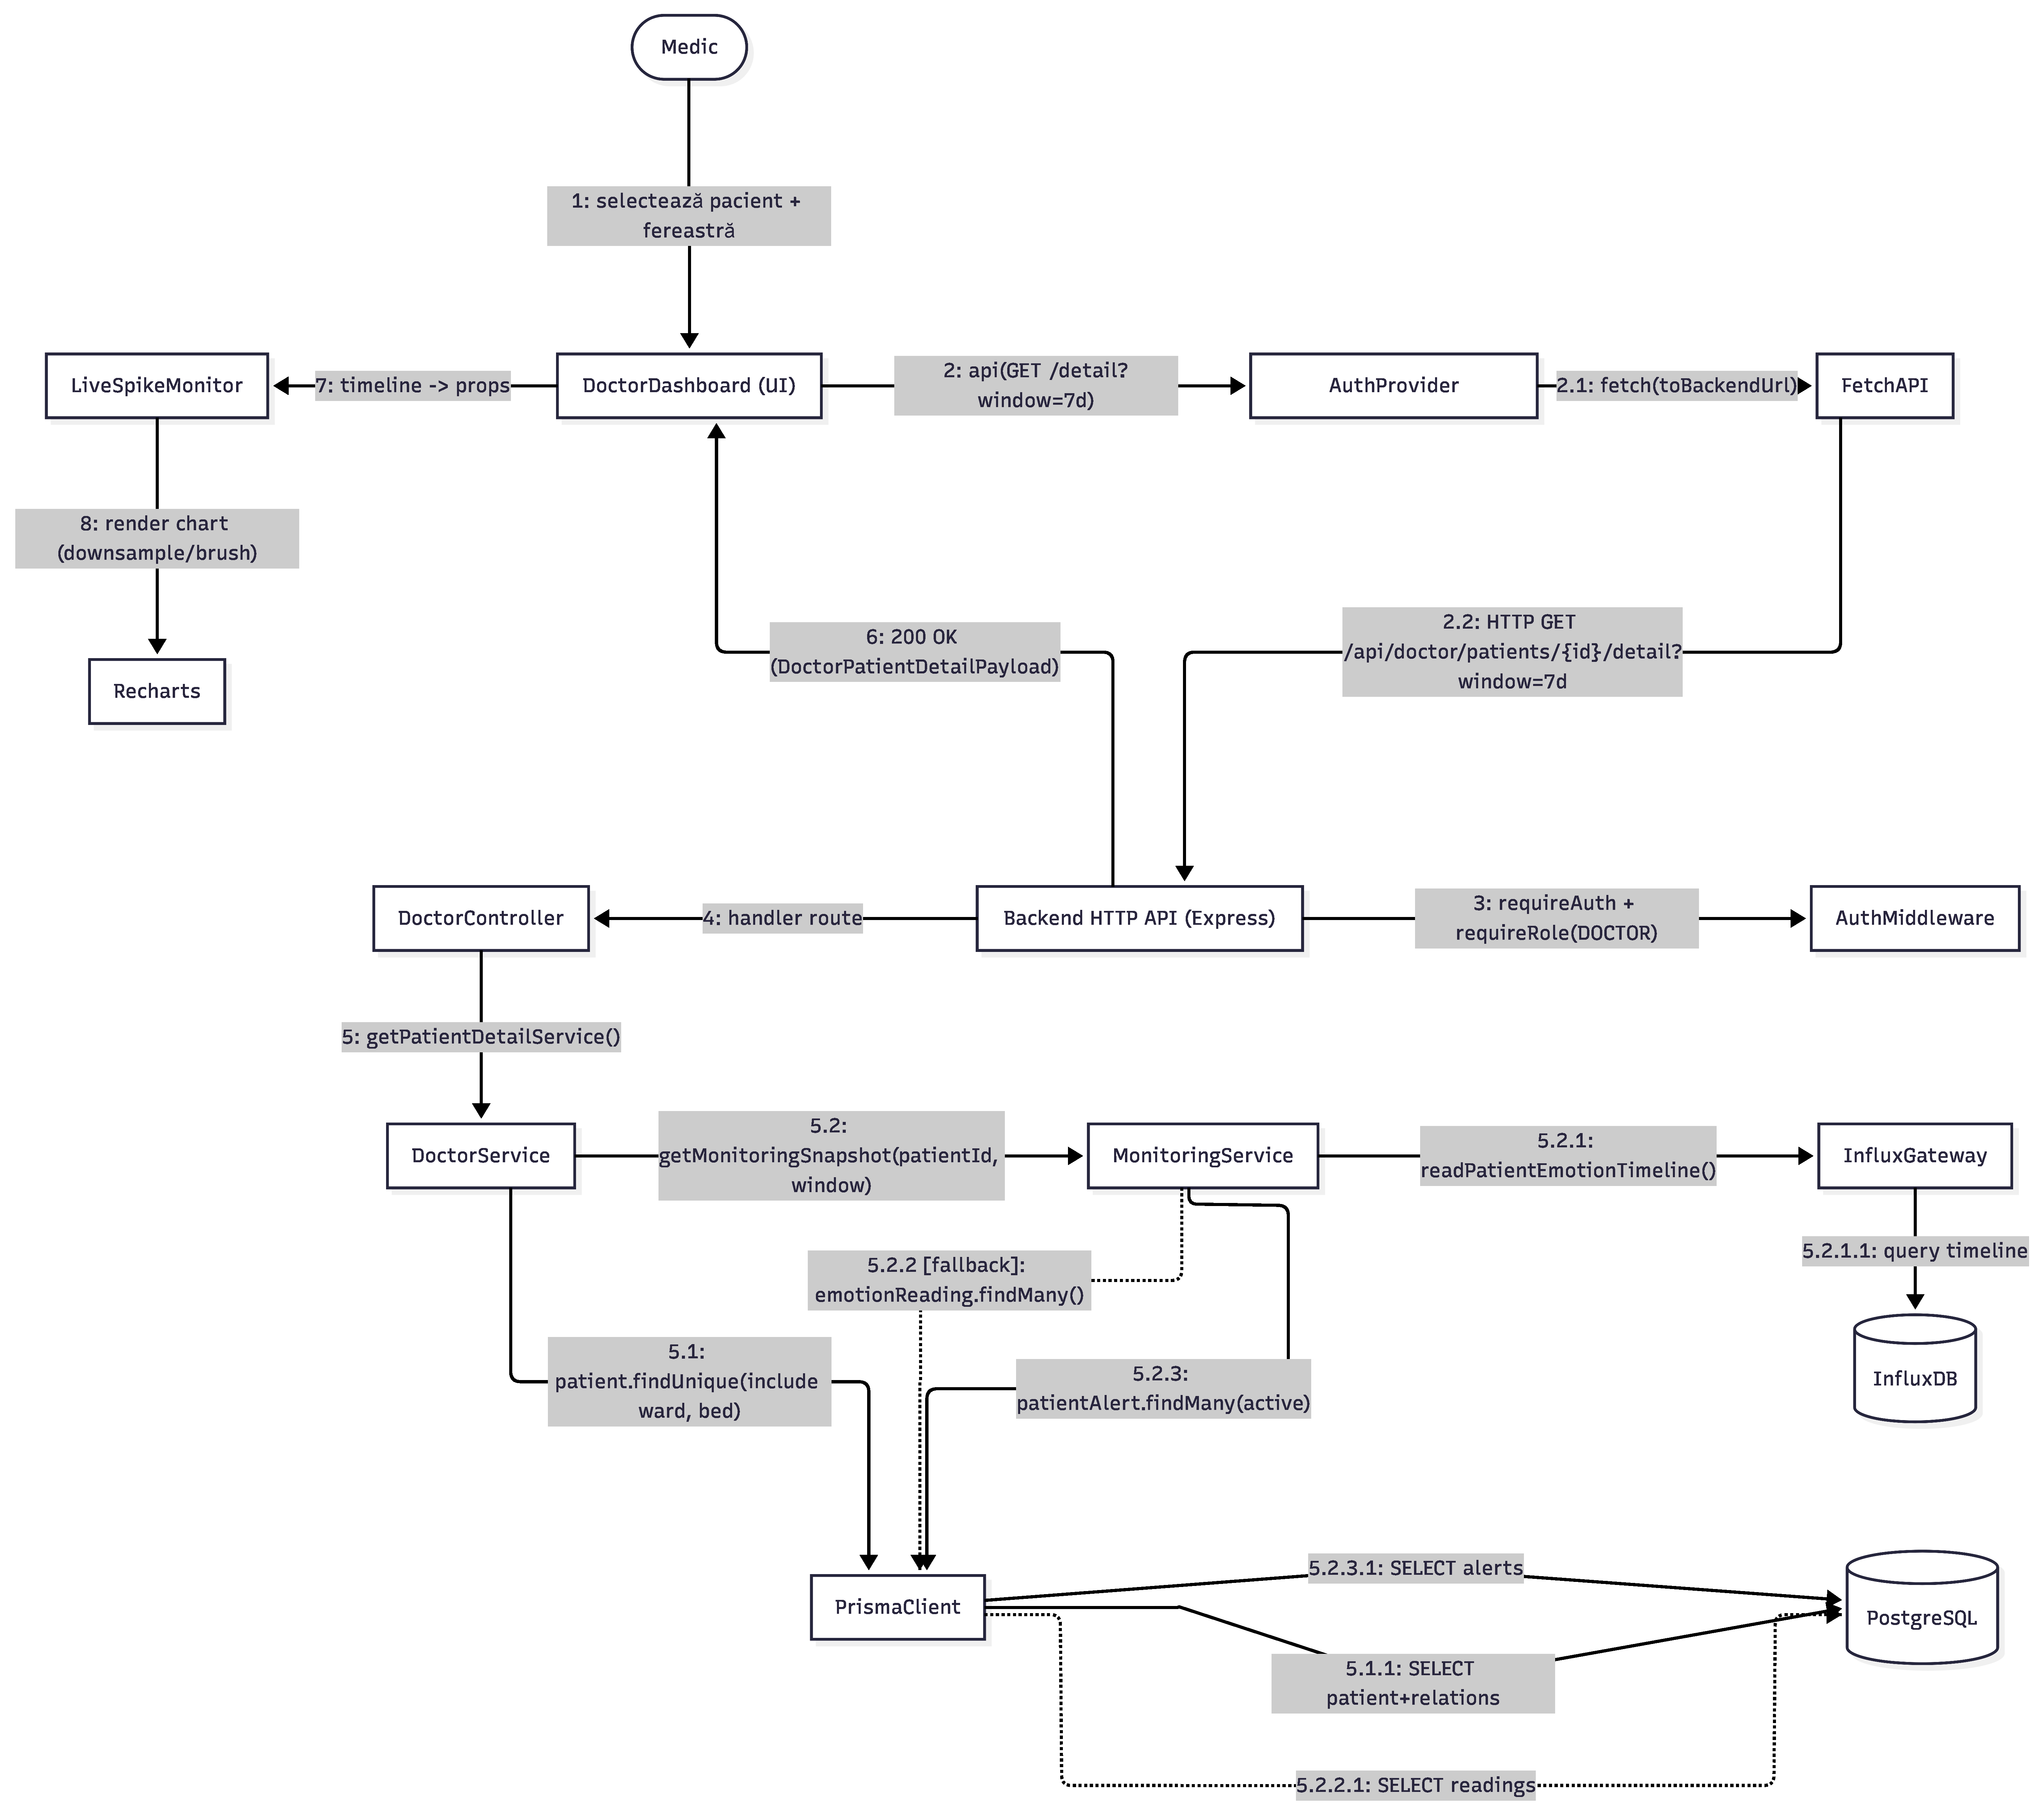
\includegraphics[width=0.7\textwidth]{figures/diagrams/diagrama-CD.pdf}
  \caption{Diagrama de comunicare pentru use case-ul \textit{Vizualizare timeline}.}
  \label{fig:comm-timeline}
\end{figure}

Figura~\ref{fig:comm-timeline} evidențiază participanții și dependențele dintre ei pentru afișarea timeline-ului clinic. Interfața medicului declanșează cererea \texttt{/detail}, autorizată prin token JWT, proces prin care backend-ul orchestrează încărcarea metadatelor pacientului și a istoricului de monitorizare. Datele istorice, denumite \texttt{timelineHistory}, sunt preluate preferențial din \textit{InfluxDB} via \textit{gateway}, aplicându-se un mecanism de \textit{fallback} pe \textit{PostgreSQL} în cazul indisponibilității bazei de date temporale. La fiecare nouă inferență de emoții aceste date istorice sunt actualizate prin adăugarea ultimelor probabilități primite. Pentru a asigura continuitatea vizuală a graficului și o experiență de utilizare fluidă, sistemul implementează un mecanism de eșantionare locală la nivelul interfeței. Astfel, la fiecare $500$ ms, buffer-ul local de memorie, \texttt{emotionHistory} — care reține datele din ultimele $65$ de minute — este actualizat prin adăugarea de noi puncte de date. În intervalele în care nu sunt recepționate cadre noi de la motorul de inferență AI, valorile emoțiilor sunt menținute constante, corespunzând ultimelor probabilități identificate. Matematic, acest comportament este echivalent cu un filtru de menținere de ordin zero (\textit{Zero-Order Hold}), unde valoarea funcției de stare $E(t)$ rămâne invariantă între două momente de detecție succesive $t_n$ și $t_{n+1}$:\begin{equation}E(t) = E(t_n), \quad \text{pentru} \quad t_n \leq t < t_{n+1}\label{eq:zoh_emotions}\end{equation}În final, payload-ul vizualizat de medic reprezintă o concatenare (\textit{mergedMonitorHistory}) a celor două fluxuri: \texttt{timelineHistory} (datele persistate) și \texttt{emotionHistory} (datele curente din memoria volatilă). Acest set de date unificat este mapat către componenta \textit{LiveSpikeMonitor}, care utilizează biblioteca \textit{Recharts} pentru randarea graficului în timp real, oferind o rezoluție de $0.5$ secunde. Un exemplu vizual intuitiv este oferit în Figura~\ref{fig:visual-timeline}. Alertele actualizate sunt folosite de mecanismul de notificări pentru a anunța doctorul schimbări importante legate de starea emoțională a pacientului. 

\begin{figure}[htbp]
  \centering
  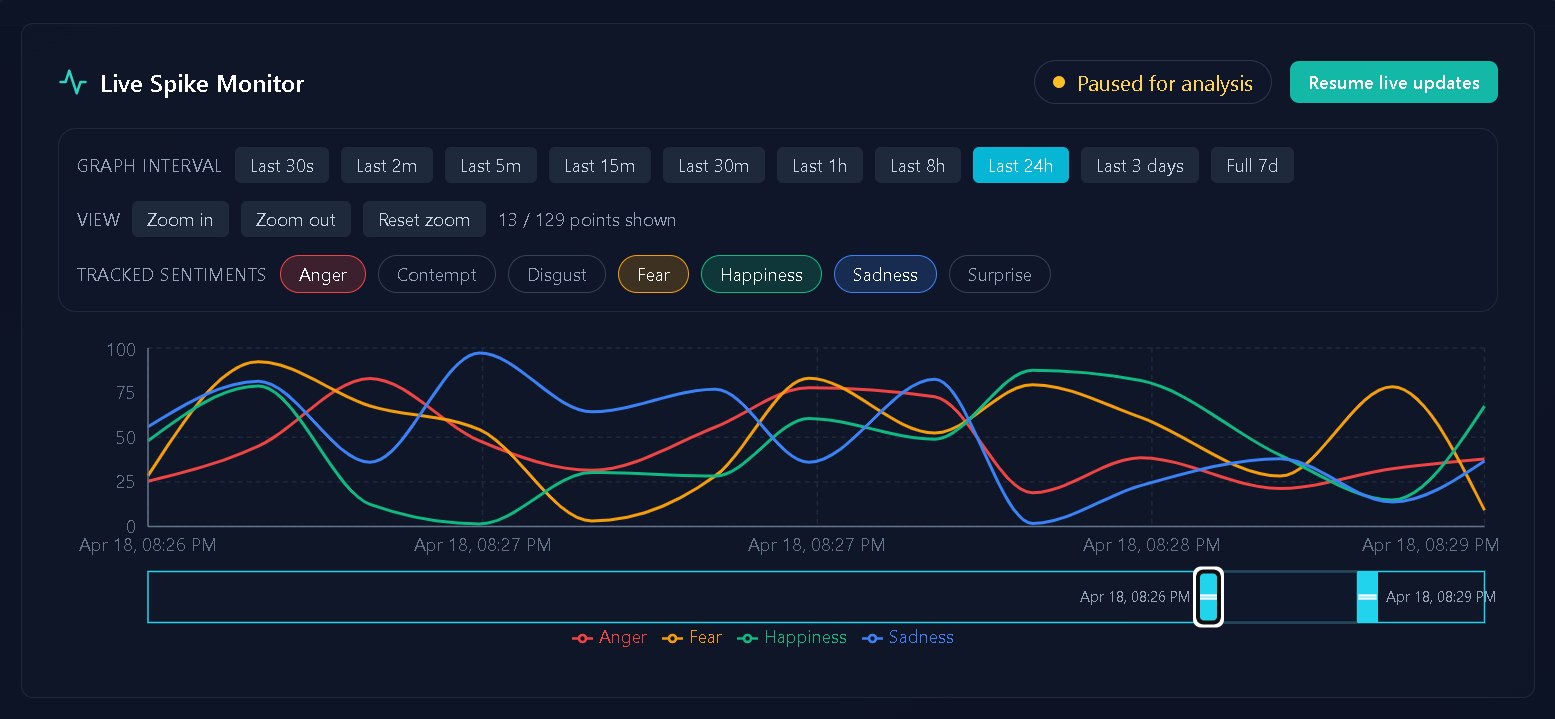
\includegraphics[width=0.99\textwidth]{figures/app/live-spike-monitor.png}
  \caption{Exemplu de vizualizare timeline.}
  \label{fig:visual-timeline}
\end{figure}

\subsection{Diagrama de deployment}
\label{subsec:model-structural-deployment}

\begin{figure}[htbp]
  \centering
  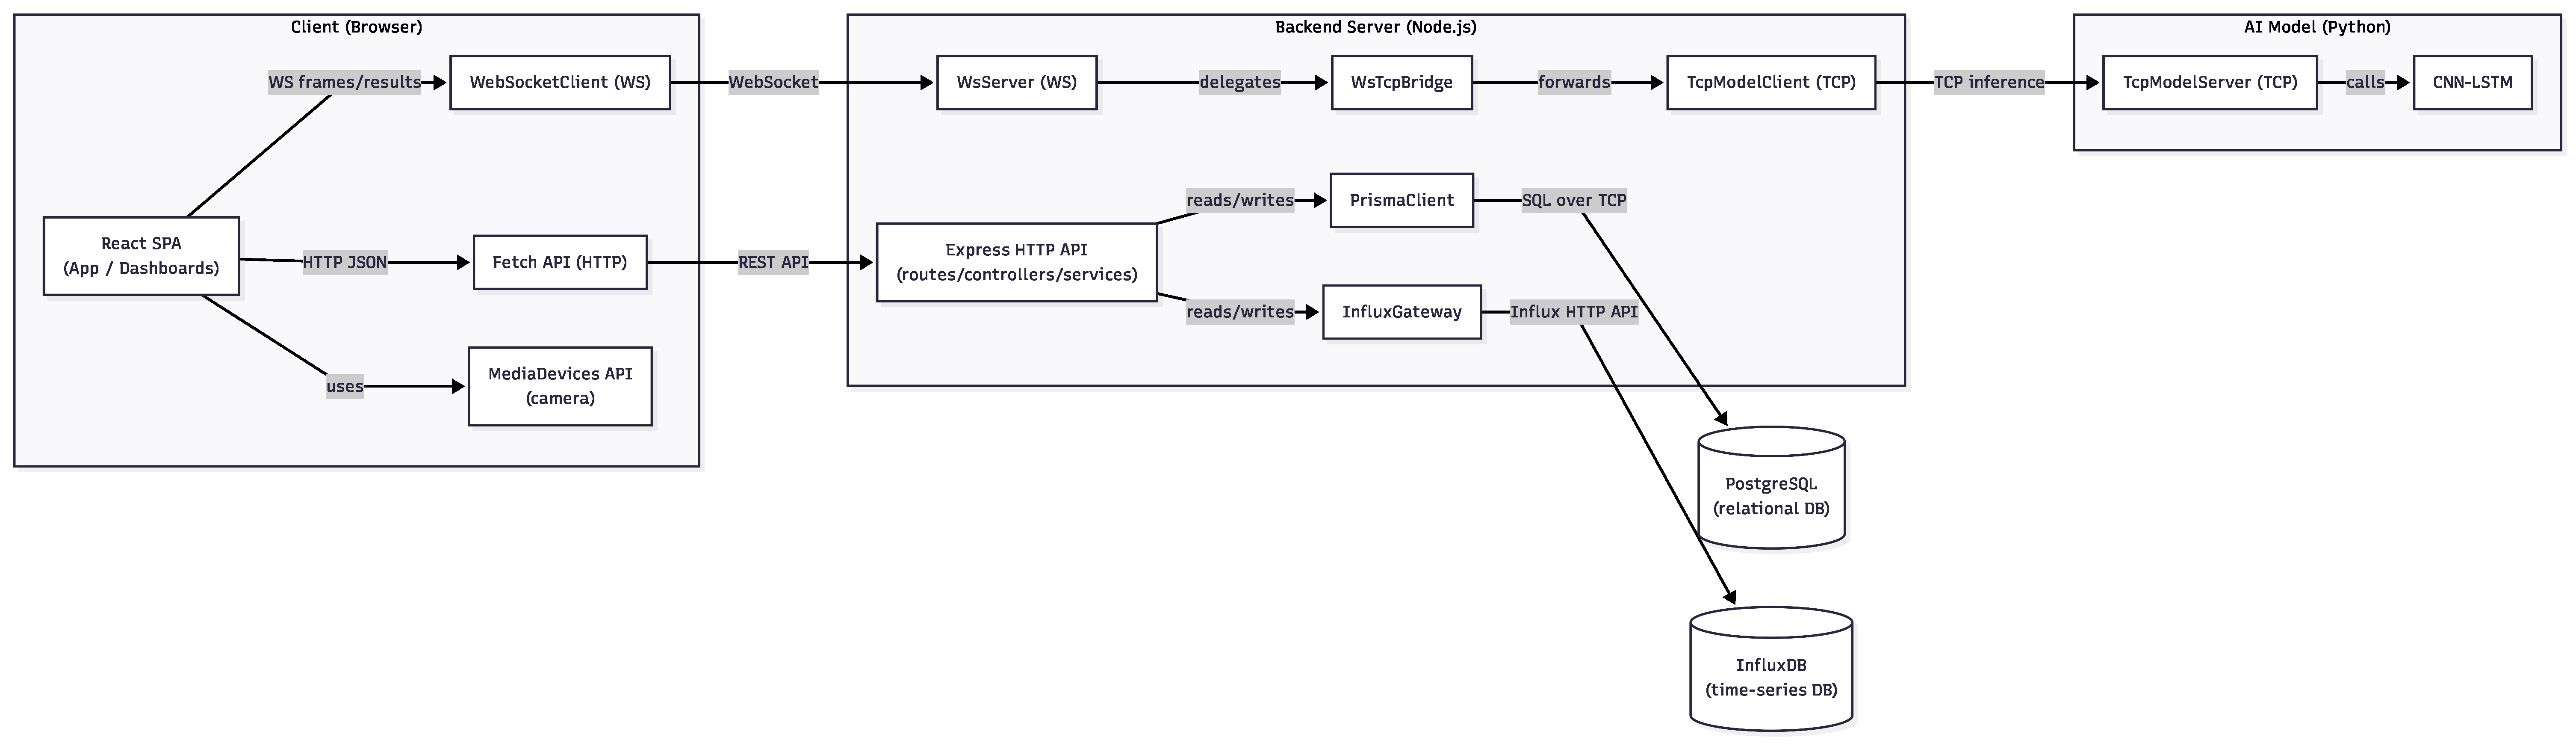
\includegraphics[width=0.99\textwidth]{figures/diagrams/diagrama-deployment.pdf}
  \caption{Diagrama de deployment: noduri de execuție și protocoale de comunicare (REST/HTTP, WebSocket, TCP).}
  \label{fig:deployment}
\end{figure}

Figura~\ref{fig:deployment} evidențiază distribuția fizică a sistemului: aplicația web rulează în browser (interfața React) și comunică cu backend-ul Node.js atât sincron prin REST/HTTP (pentru operații CRUD și încărcarea datelor), cât și asincron prin WebSocket (pentru streaming de cadre și rezultate). Backend-ul accesează persistența relațională în PostgreSQL prin Prisma și utilizează InfluxDB ca depozit time-series pentru timeline-uri, iar inferența este externalizată către un server de model dedicat, accesat prin TCP. Între TCP și WS există o punte de legătură (\textit{TsTcpBridge}) ce asigură comunicarea între cele 2 protocoale.

\subsubsection{Motivația utilizării PostgreSQL + InfluxDB}
\label{subsubsec:postgres-influx-motivatie}

Pentru persistență am ales o abordare hibridă, separând datele \textbf{tranzacționale} (structurate, cu relații) de datele
\textbf{time-series} (flux continuu de puncte indexate temporal). Această separare reduce cuplarea dintre workload-ul de tip OLTP
(operare zilnică, integritate, actualizări) și workload-ul de tip analiză temporală (range queries, agregări pe ferestre).

\begin{itemize}
  \item \textbf{PostgreSQL (bază relațională, sursa de adevăr pentru domeniu clinic).}
  PostgreSQL este utilizat pentru entitățile cu relații clare și reguli de consistență: utilizatori și roluri,
  pacienți, alocarea în salon/pat, stări operaționale, respectiv alertele persistente. Acest tip de date beneficiază direct de:
  \textit{ACID transactions}, constrângeri (chei primare/străine), modelare normalizată, interogări cu \textit{JOIN}-uri și
  migrații controlate ale schemei. Într-un context clinic, aceste proprietăți sunt importante pentru a evita stări invalide
  (ex. pacient fără pat/ward valid sau alerte asociate greșit) și pentru a păstra un istoric coerent.

  \item \textbf{InfluxDB (TSDB pentru timeline-uri și interogări pe intervale de timp).}
  Pentru monitorizarea emoțiilor, aplicația produce un volum mare de puncte cu timestamp (emoții + scoruri derivate),
  interogate aproape exclusiv pe ferestre de timp (ex. ultimele 24h sau 7 zile) și afișate ca grafice.
  O bază de date time-series este optimizată pentru acest tip de acces:
  (i) scrieri frecvente și eficiente, (ii) compresie și stocare eficientă pentru date temporale,
  (iii) interogări rapide de tip \textit{range scan} (``toate punctele dintre $t_0$ și $t_1$''),
  (iv) posibilitatea de a aplica politici de retenție și/sau downsampling fără a afecta modelul relațional.
\end{itemize}

\noindent\textbf{Eficiență și izolare a performanței.}
Deși datele time-series pot fi păstrate și într-o bază relațională, pe măsură ce crește frecvența de eșantionare și retenția,
tabelele mari pot introduce costuri suplimentare (indexuri mai voluminoase, operații de mentenanță, impact asupra latențelor OLTP).
Prin utilizarea InfluxDB pentru timeline-uri, încărcarea asociată interogărilor temporale este mutată către un motor dedicat,
menținând backend-ul și baza relațională responsive pentru operațiile critice (CRUD și tranzacții).

\noindent\textbf{Robustețe operațională (fallback).}
Arhitectura permite ca timeline-ul să fie citit cu prioritate din InfluxDB (dacă este disponibil și are puncte),
iar în caz contrar din persistența relațională; astfel, sistemul rămâne funcțional chiar și în situații de configurare incompletă
sau indisponibilitate temporară a depozitului time-series.

\subsection{Diagrama de stare: \textit{PatientAlert}}
\label{subsec:model-dinamic-stare-patientalert}

\begin{figure}[htbp]
  \centering
  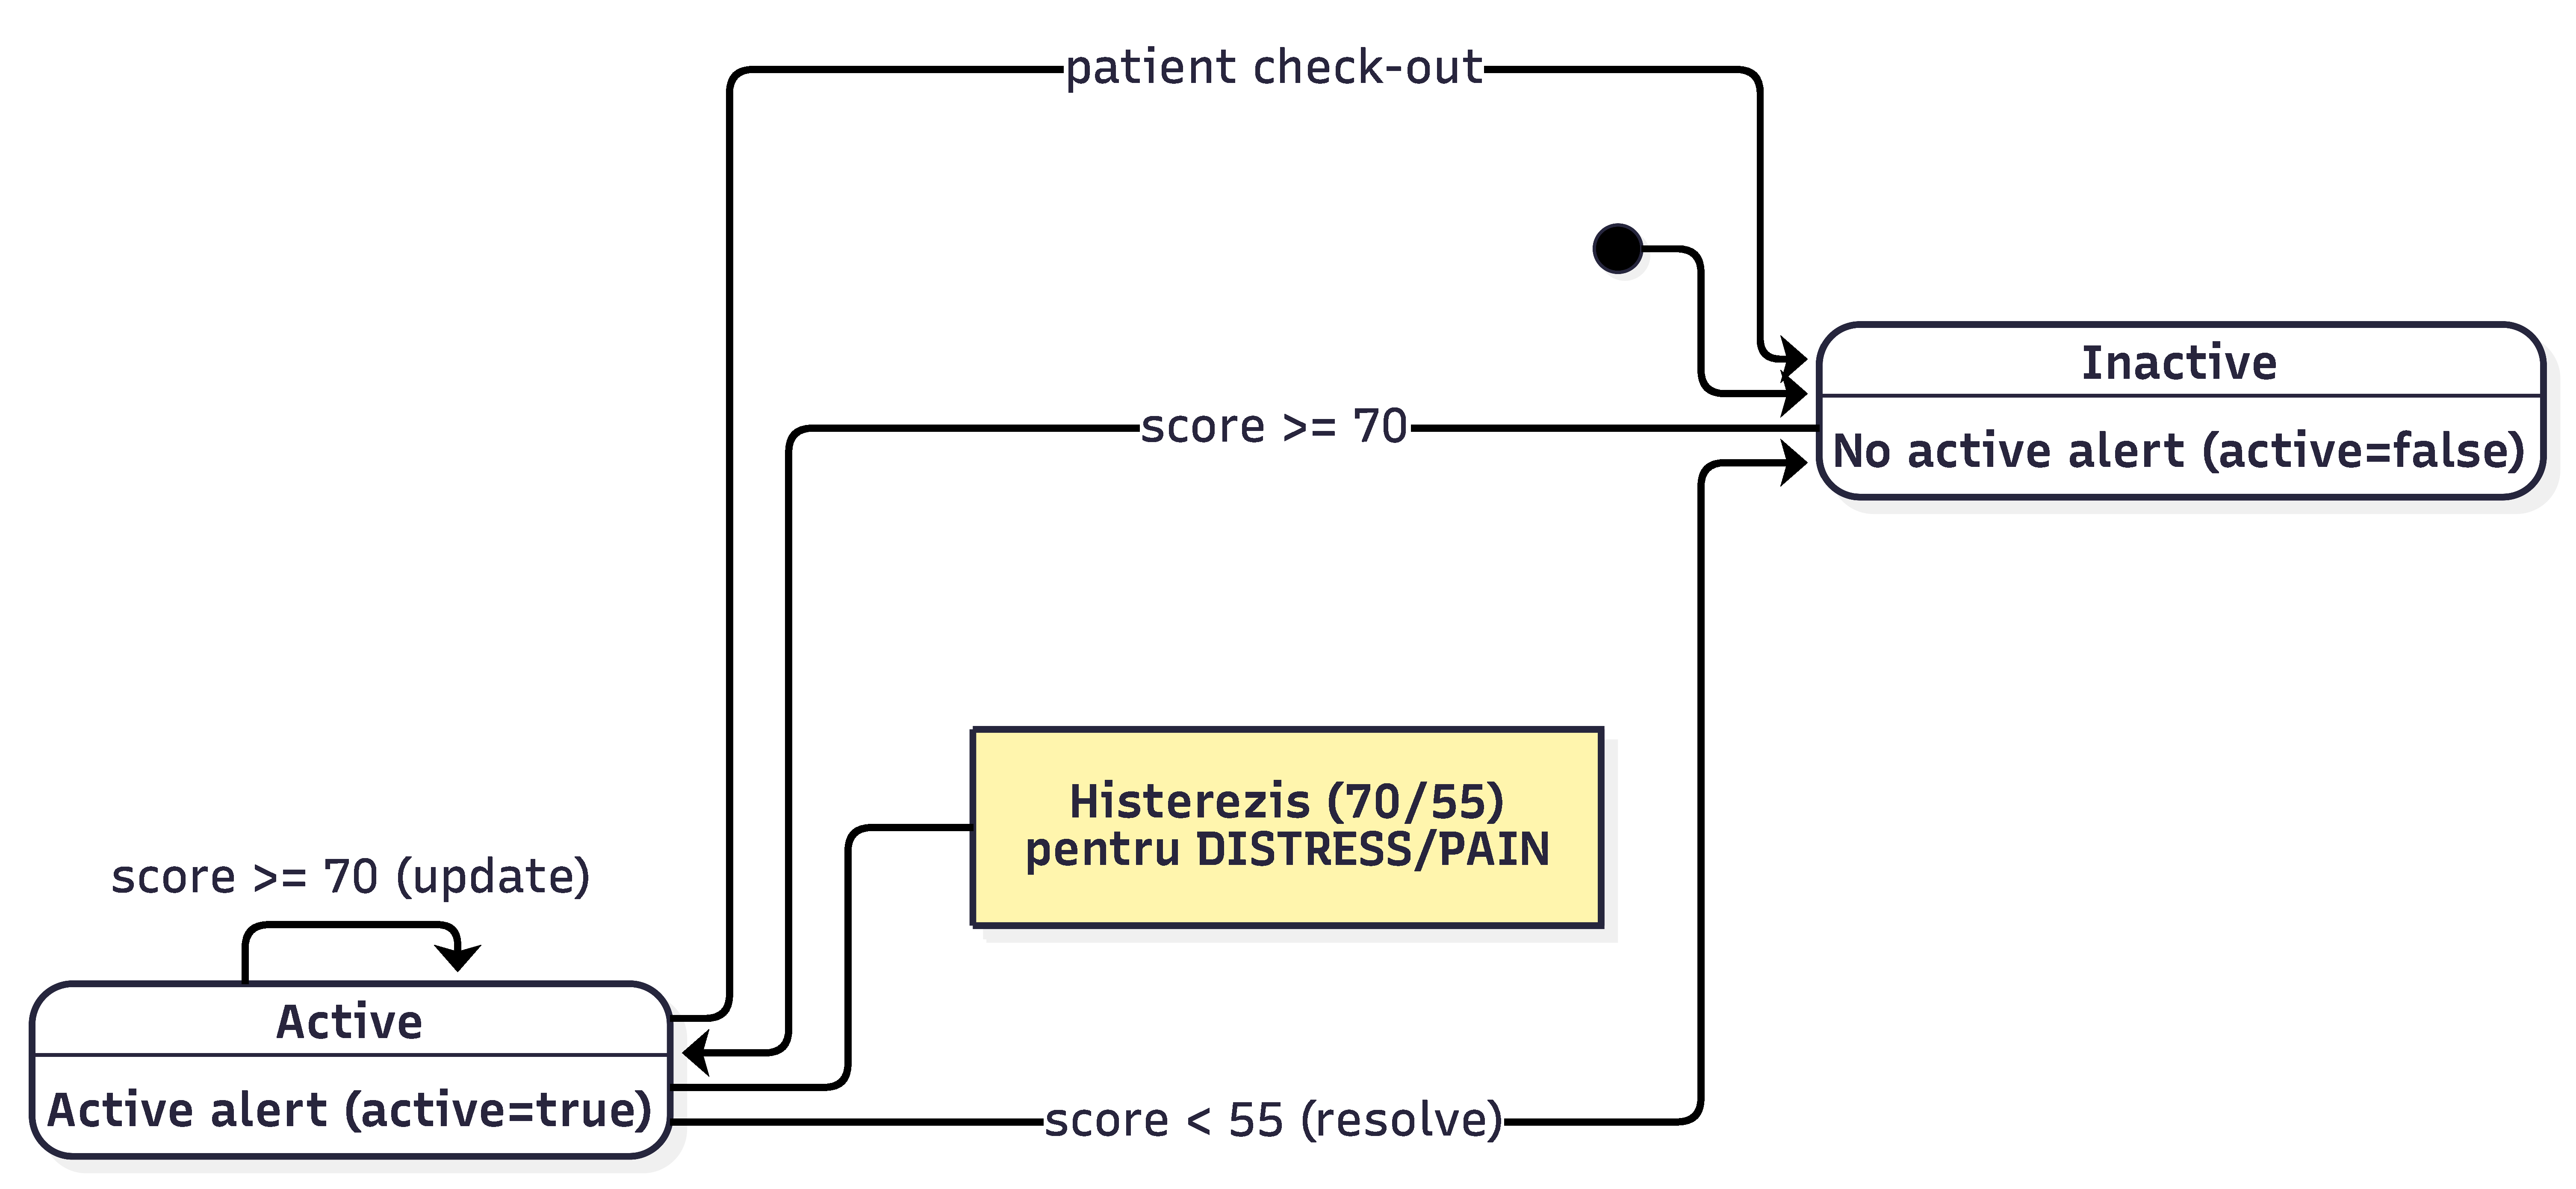
\includegraphics[width=0.6\textwidth]{figures/diagrams/diagrama-stari.pdf}
  \caption{Diagrama de stare pentru \textit{PatientAlert} (per pacient și tip de alertă).}
  \label{fig:state-patientalert}
\end{figure}

Figura~\ref{fig:state-patientalert} descrie ciclul de viață al unei alerte clinice (\textit{DISTRESS}/\textit{PAIN}) asociate unui pacient. Pentru optimizarea mecanismului de declanșare a alertelor și eliminarea fenomenului de instabilitate (\textit{jitter}) la pragurile de decizie, a fost implementat un algoritm de \textbf{histerezis} detaliat în Figura \ref{fig:histerezis_logic}. Acesta utilizează praguri diferențiate pentru activarea ($T_{high} = 70$) și dezactivarea ($T_{low} = 55$) stării de alertă, asigurând astfel o stabilitate temporală a monitorizării și reducând oscilațiile frecvente ale stării.

\begin{figure}[htbp]
    \centering
    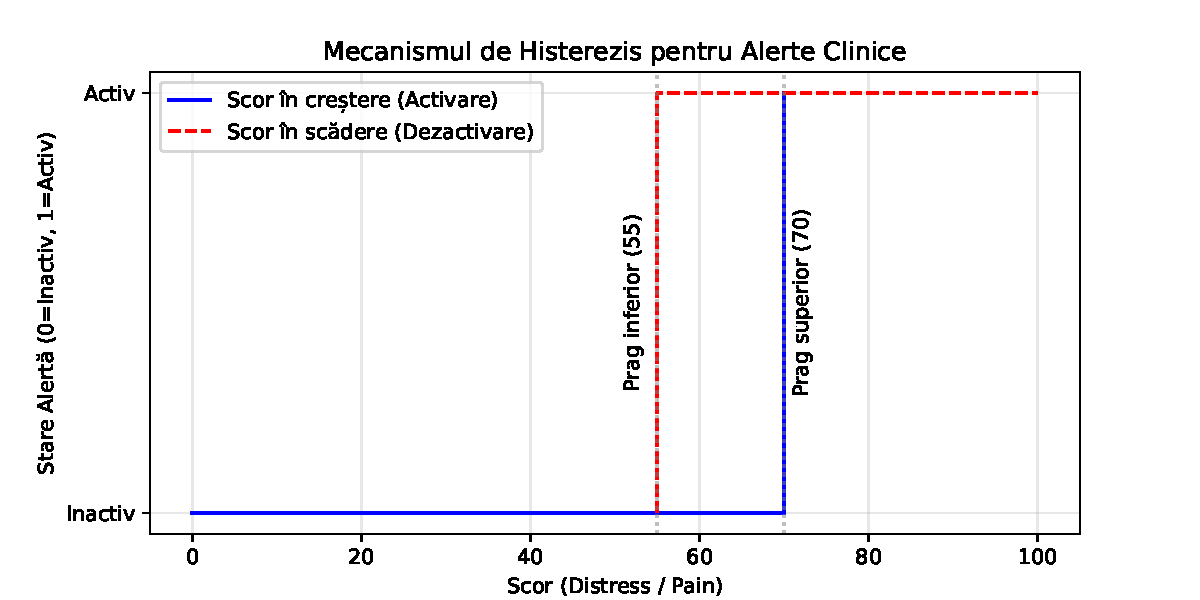
\includegraphics[width=0.8\textwidth]{figures/histerezis_alerte.pdf}
    \caption{Reprezentarea grafică a mecanismului de histerezis aplicat sistemului de alerte. Activarea se produce la depășirea pragului de $70$, în timp ce revenirea la starea inactivă necesită scăderea scorului sub $55$.}
    \label{fig:histerezis_logic}
\end{figure}

Calculul severității se bazează pe două metrici fundamentale, derivate din vectorul stărilor emoționale detectate ($V$). Prima metrică, scorul de \textbf{Distress} ($S_D$), este calculată ca medie aritmetică a stărilor de furie, frică și tristețe, conform ecuației~\eqref{eq:distress_score}:

\begin{equation}
    S_D = \text{clamp}\left(\frac{V_{\text{anger}} + V_{\text{fear}} + V_{\text{sadness}}}{3}, 0, 100\right)
    \label{eq:distress_score}
\end{equation}

Cea de-a doua metrică, scorul de \textbf{Pain} ($S_P$), reprezintă o medie ponderată ce prioritizează frica și tristețea ca indicatori non-verbali ai suferinței fizice, fiind definită în relația~\eqref{eq:pain_score}:

\begin{equation}
    S_P = \text{clamp}\left(0.45 \cdot V_{\text{fear}} + 0.4 \cdot V_{\text{sadness}} + 0.15 \cdot V_{\text{disgust}}, 0, 100\right)
    \label{eq:pain_score}
\end{equation}

În scenariul în care ambele scoruri calculate prin formulele~\eqref{eq:distress_score} și \eqref{eq:pain_score} depășesc pragul critic de activare ($T_{high}$), sistemul aplică o logică de arbitrare prin selecția valorii maxime. Astfel, intensitatea și eticheta alertei sunt determinate de scorul final ($S_{final}$), determinat conform relației~\eqref{eq:final_score}:

\begin{equation}
    S_{final} = \max(S_D, S_P)
    \label{eq:final_score}
\end{equation}

O alertă trece în starea \textit{Active} atunci când valoarea rezultată din ecuația~\eqref{eq:final_score} respectă condiția $S_{final} \geq 70$. În timpul stării active, severitatea și mesajul sunt actualizate dinamic pe baza noilor citiri. Pentru a evita declanșarea repetitivă a notificărilor la fluctuații minore, rezolvarea alertei se produce doar atunci când $S_{final} < 55$, moment în care alertarea este dezactivată și se înregistrează timpul de rezolvare.
Toate aceste actualizări au loc la persistarea unui nou reading de emoții, backendul calculând severitatea pe baza scorului:
  \begin{itemize}
    \item \texttt{HIGH} dacă $\text{score} \ge 85$,
    \item \texttt{MEDIUM} dacă $\text{score} \ge 72$,
    \item \texttt{LOW} în caz contrar.
  \end{itemize}
În interfață, aceste alerte sunt afișate în \textit{Clinical Insights} la secțiunea \textit{Current Alerts} (Figura~\ref{fig:current-alerts}) și reprezintă starea clinică persistată pentru pacient (pe intervalele recente de funcționare).

Sistemul calculează și alerte \textbf{derivate} (nepersistate), pe baza unui \textit{timeline} de emoții pe o fereastră de timp
(ex. 24h sau 7d). Aceste alerte urmăresc episoade susținute, nu doar vârfuri scurte:

\begin{itemize}
  \item Se generează o alertă de tip \texttt{DISTRESS} sau \texttt{PAIN} dacă scorul corespunzător rămâne peste \textbf{65\%}
        timp de cel puțin \textbf{60 minute}.
  \item Mesajul include durata episodului și vârful (peak) atins în acea perioadă.
  \item Severitatea este calculată după aceeași logică (HIGH/MEDIUM/LOW) în funcție de peak.
\end{itemize}

În interfață, aceste alerte apar în \textit{Clinical Insights} la secțiunea \textit{Prolonged Alerts} (Figura~\ref{fig:prolonged-alerts}) și sunt recalculte la fiecare
obținere a unui nou \textit{snapshot} de monitorizare din backend.

\begin{figure}[htbp]
    \centering
    \begin{minipage}{0.48\textwidth}
        \centering
        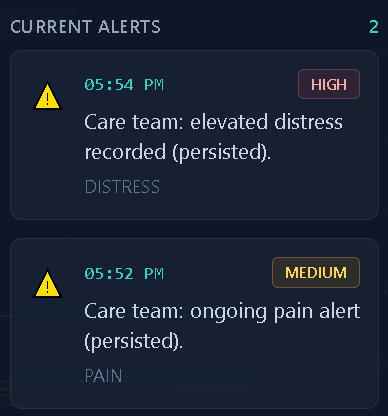
\includegraphics[width=\textwidth]{figures/app/current-alerts.png}
        \caption{Secțiunea \textit{Current Alerts} - vizualizarea alertelor persistente.}
        \label{fig:current-alerts}
    \end{minipage}
    \hfill
    \begin{minipage}{0.48\textwidth}
        \centering
        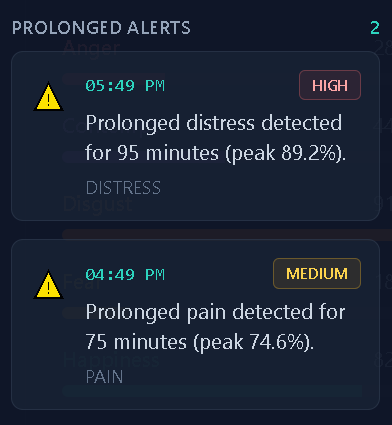
\includegraphics[width=\textwidth]{figures/app/prolonged-alerts.png}
        \caption{Secțiunea \textit{Prolonged Alerts} - vizualizarea alertelor de durată.}
        \label{fig:prolonged-alerts}
    \end{minipage}
\end{figure}

\subsection{Diagrama de activități: Check-in pacient}
\label{subsec:model-dinamic-activity-checkin}

\begin{figure}[htbp]
  \centering
  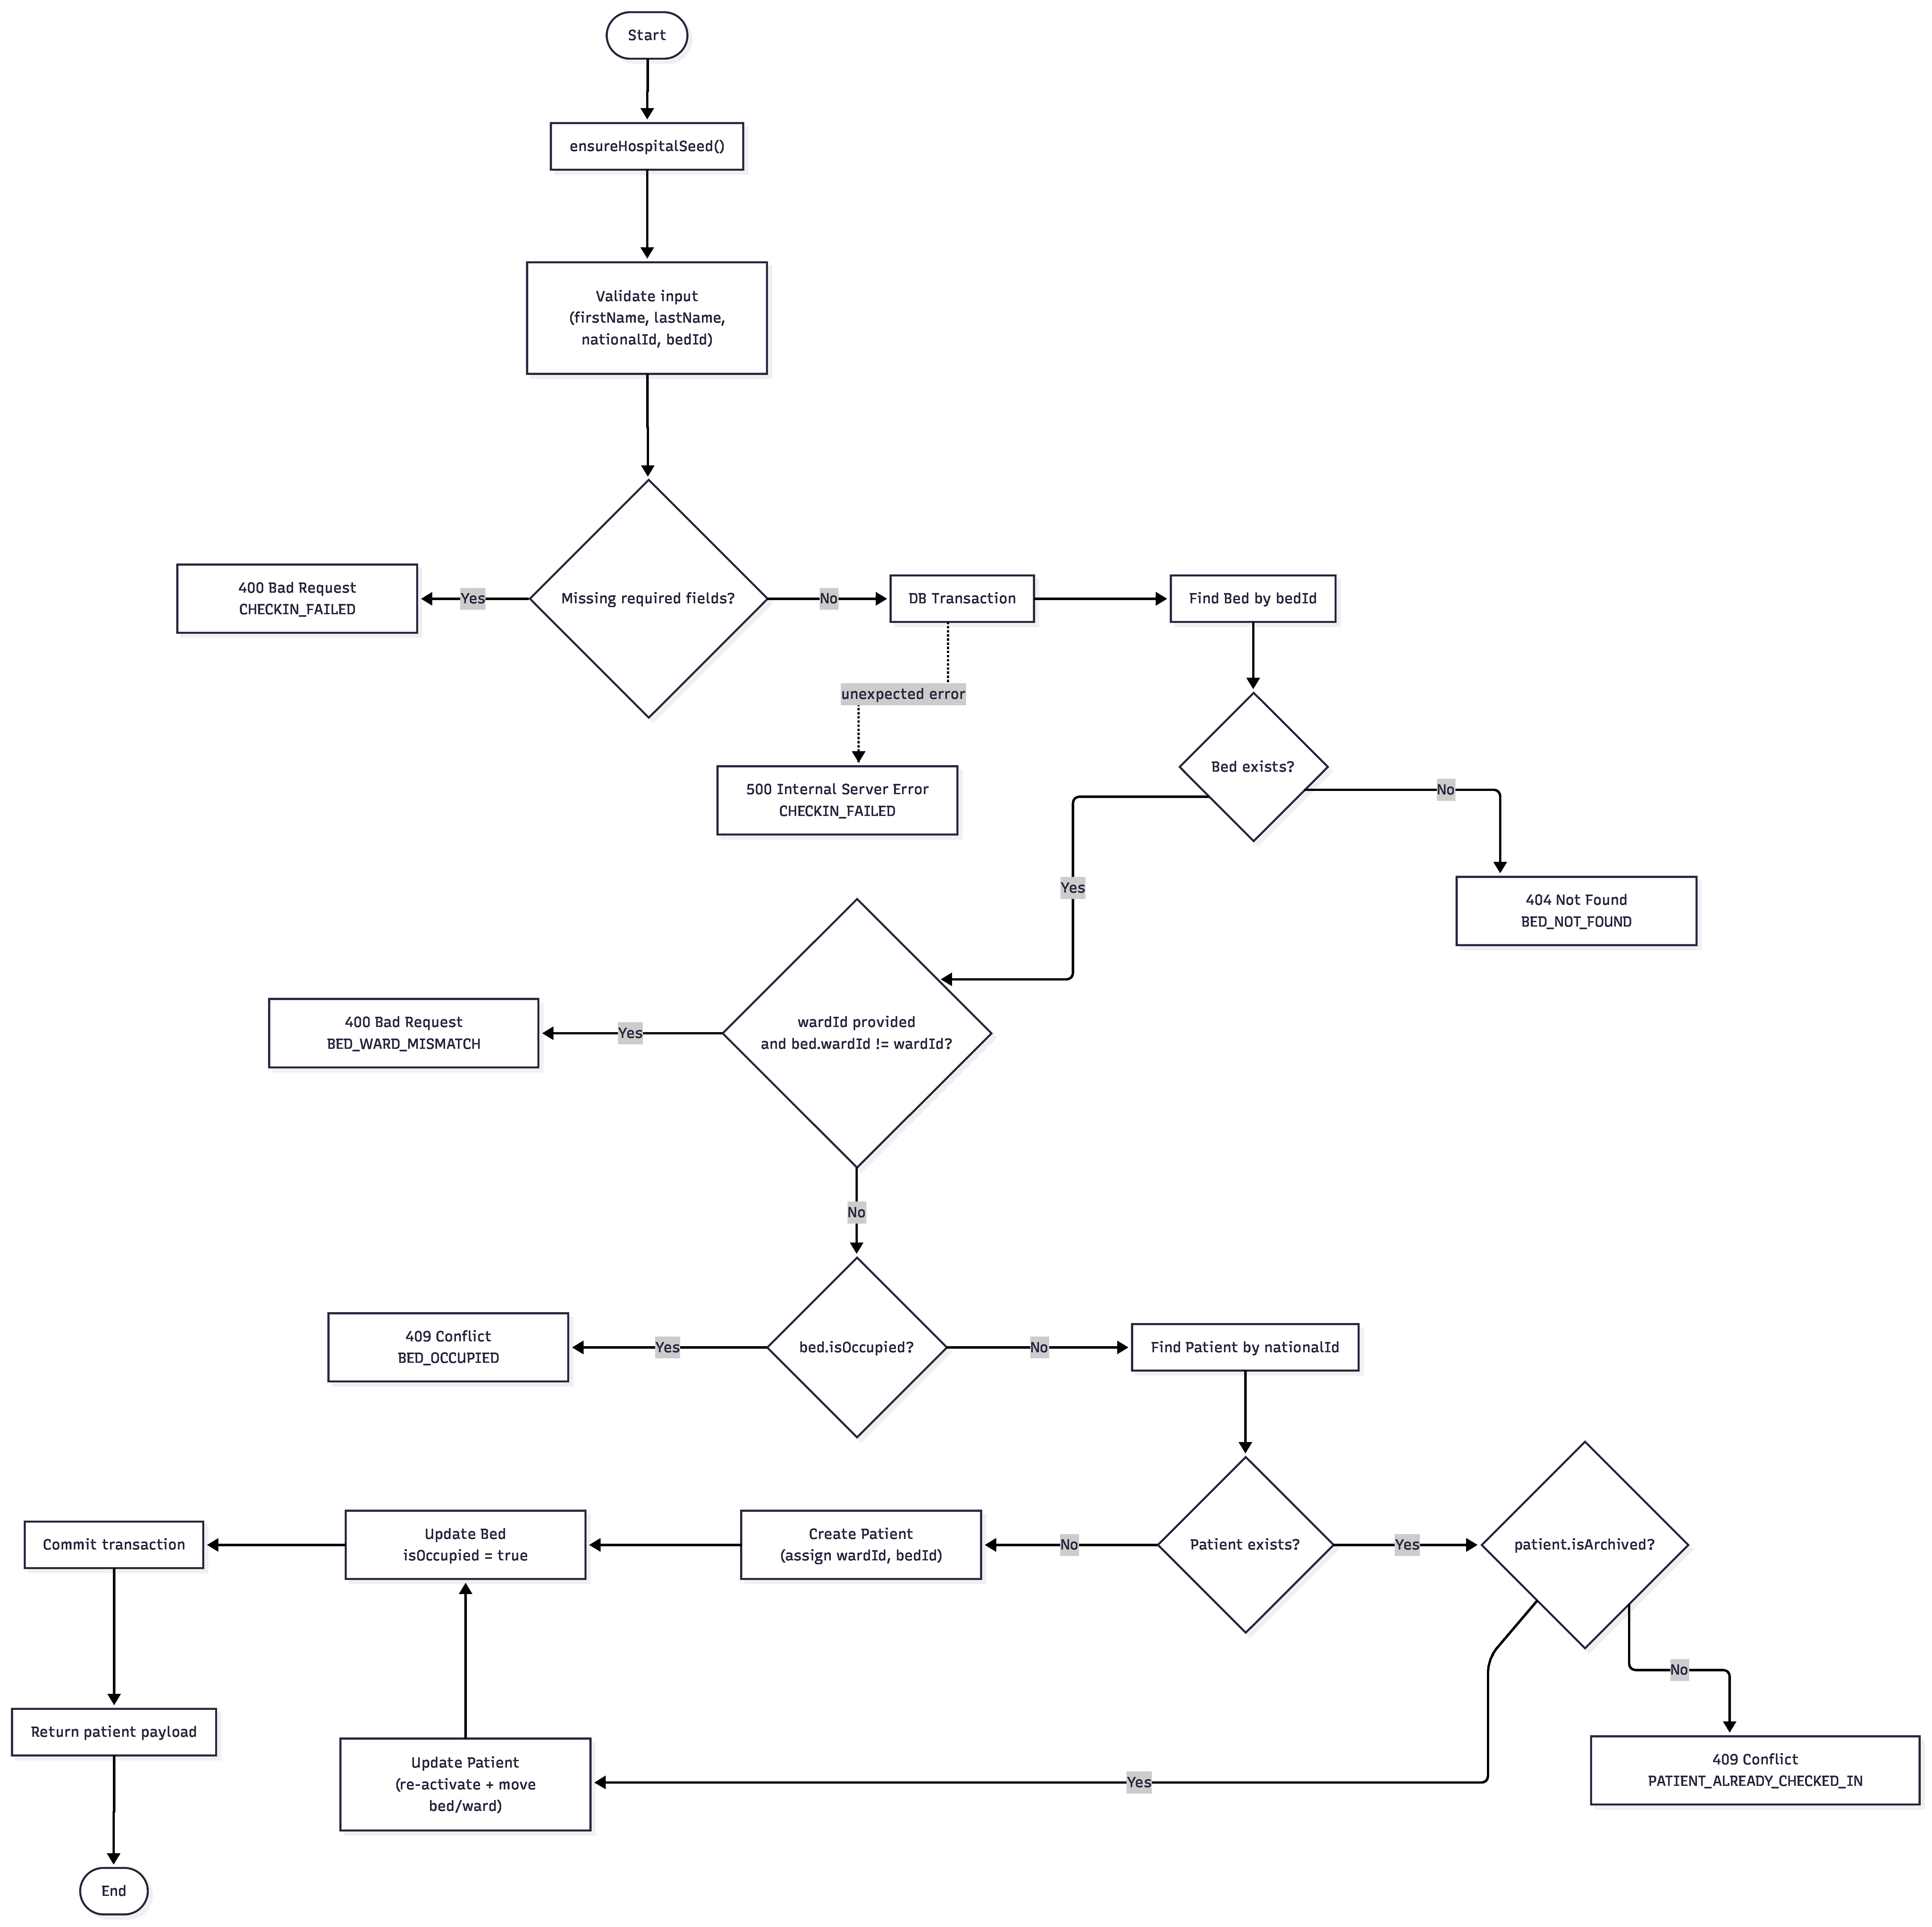
\includegraphics[width=0.97\textwidth]{figures/diagrams/diagrama-activitati.pdf}
  \caption{Diagrama de activități pentru use case-ul \textit{Check-in pacient}.}
  \label{fig:activity-checkin}
\end{figure}

Figura~\ref{fig:activity-checkin} prezintă fluxul operațional de internare (check-in) și deciziile principale care garantează consistența datelor: validarea câmpurilor obligatorii, verificarea existenței patului, compatibilitatea pat--secție (când se indică o secție), și prevenirea ocupării simultane. Operația este tratată tranzacțional, astfel încât înregistrarea/actualizarea pacientului și marcarea patului ca ocupat să fie aplicate atomic. În cazul unui pacient deja internat se returnează un răspuns de tip conflict, iar pentru erori neprevăzute se semnalizează eșecul operației.

\section{Sistemul de alerte și notificări}
\label{sec:sistem-alerte-notificari}

Aplicația integrează un mecanism multi-nivel de alertare, destinat în principal utilizatorului cu rol de medic.
Semnalele sunt generate atât \textbf{în timp real} (din probabilitățile inferate de model), cât și \textbf{la nivel backend}
(din istoricul pacientului și alertele persistate). În plus, există notificări operaționale (erori/stări de funcționare).

\subsection{Evenimente clinice în sesiune (Live Session Events)}
\label{subsec:live-session-events}

La recepționarea fiecărui vector de probabilități de la modelul de inferență, valorile emoționale sunt supuse unui proces de normalizare în intervalul $[0, 100]$, fiind ulterior redate în interfața medicului sub formă de procente. Această vizualizare a emoțiilor curente, exemplificată în Figura~\ref{fig:sentiment-distribution-ui}, oferă o analiză granulară a profilului afectiv, permițând identificarea rapidă a stărilor dominante și a nuanțelor emoționale ale pacientului. Simultan cu afișarea brută a datelor, sistemul execută un mecanism de analiză euristică pentru identificarea episoadelor emoționale semnificative. Se determină emoția dominantă ($E_{max}$) prin identificarea valorii maxime din setul de probabilități curente. Dacă această valoare depășește pragul critic de activare, stabilit la un nivel de încredere de $60\%$, sistemul generează automat un eveniment clinic (\textit{Clinical Event}), conform logicii descrise în relația~\eqref{eq:clinical_event_trigger}:

\begin{equation}
\text{Trigger} = \begin{cases} 
\text{generare eveniment}, & \text{daca} \text{ } \max(V_{\text{emotii}}) > 60 \\ 
\text{stare latenta}, & \text{altfel} 
\end{cases}
\label{eq:clinical_event_trigger}
\end{equation}

Structura și comportamentul acestor evenimente sunt definite prin următoarele caracteristici tehnice, așa cum reiese și din detaliile surprinse în figurile de mai jos:

\begin{itemize}
  \item \textbf{Trigger}: $\max(\text{emotii}) > 60\%$.
  \item \textbf{Conținut}: emoția dominantă, intensitatea (în \%), timestamp și un mesaj selectat aleator din 3 variante predefinite (pentru a evita repetitivitatea).
  \item \textbf{Afișare}: evenimentele apar în panoul \textit{Clinical Insights} la secțiunea \textit{Live Session Events}.
  \item \textbf{Feedback vizual}: emoția detectată este evidențiată temporar (efect de tip \textit{flash/pulse}).
\end{itemize}

\begin{figure}[htbp]
    \centering
    \begin{minipage}{0.35\textwidth}
        \centering
        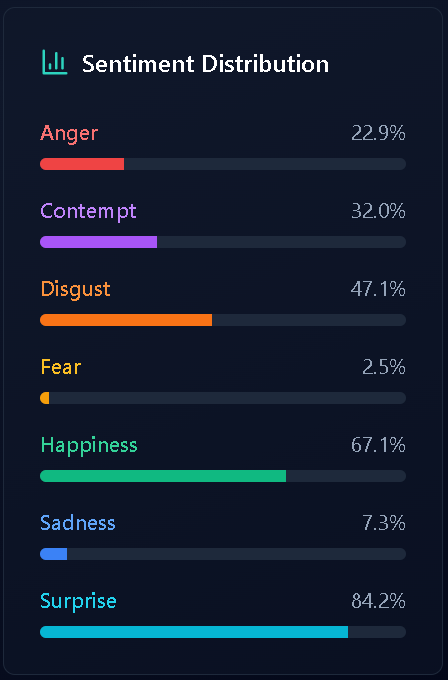
\includegraphics[width=\textwidth]{figures/app/sentiment-distribution.png}
        \caption{Vizualizarea emoțiilor și a intensităților curente.}
        \label{fig:sentiment-distribution-ui}
    \end{minipage}
    \hfill
    \begin{minipage}{0.50\textwidth}
        \centering
        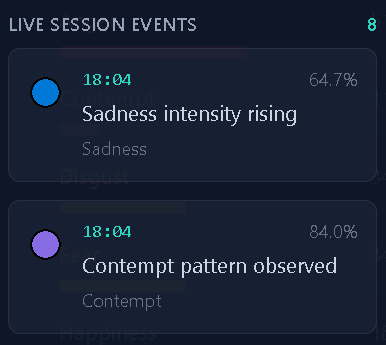
\includegraphics[width=\textwidth]{figures/app/clinical-events.png}
        \caption{Detaliu al panoului \textit{Clinical Insights} cu evenimentele generate.}
        \label{fig:clinical-events-panel}
    \end{minipage}
\end{figure}


\subsection{Indicatori rezumați în UI}
\label{subsec:ui-indicators}

\subsubsection{Clinical Risk Level (Low / Medium / High)}
\label{subsubsec:clinical-risk-level}

În \textit{Patient Sidebar} se afișează nivelul rezumat de risc clinic (\textit{Clinical Risk Level}), derivat din media emoțiilor negative:

\begin{equation}
  \text{avgNegative} = \frac{\text{Anger} + \text{Fear} + \text{Sadness}}{3}
\end{equation}

\begin{equation}
\text{riskLevel} =
\begin{cases}
\text{High}, & \text{dacă } \text{avgNegative} > 50 \\
\text{Medium}, & \text{dacă } \text{avgNegative} > 25 \\
\text{Low}, & \text{altfel}
\end{cases}
\end{equation}

Exemplele vizuale pentru cele trei niveluri sunt prezentate în Figura~\ref{fig:risk-levels}.

\begin{figure}[htbp]
  \centering
  \begin{subfigure}[t]{0.31\textwidth}
    \centering
    
\includegraphics[width=\linewidth]{figures/app/low-clinical-risk-level.png}
    \caption{Low}
    \label{fig:risk-low}
  \end{subfigure}\hfill
  \begin{subfigure}[t]{0.36\textwidth}
    \centering
    
\includegraphics[width=\linewidth]{figures/app/medium-clinical-risk-level.png}
    \caption{Medium}
    \label{fig:risk-medium}
  \end{subfigure}\hfill
  \begin{subfigure}[t]{0.31\textwidth}
    \centering
    
\includegraphics[width=\linewidth]{figures/app/high-clinical-risk-level.png}
    \caption{High}
    \label{fig:risk-high}
  \end{subfigure}
  \caption{Nivelul de risc clinic (Clinical Risk Level) în cele trei stări.}
  \label{fig:risk-levels}
\end{figure}

\subsubsection{Session Type (normal / positive / high-risk)}
\label{subsubsec:session-type}

În header-ul aplicației (lângă titlul platformei) este afișat \textit{Session Type}, care sintetizează rapid starea sesiunii.
Acesta este determinat combinând alertele clinice și emoțiile curente:

\begin{itemize}
  \item \textbf{High-risk}: dacă există cel puțin o alertă cu severitate \texttt{HIGH} (din \textit{Current} sau \textit{Prolonged Alerts})
        \textbf{sau} dacă $\text{Anger} > 60$ și $\text{Fear} > 60$.
  \item \textbf{Positive}: dacă $\text{Happiness} > 50$ și $\text{Surprise} > 30$.
  \item \textbf{Normal}: în celelalte situații.
\end{itemize}

Exemplele vizuale pentru cele trei tipuri sunt prezentate în Figura~\ref{fig:session-types}.

\begin{figure}[htbp]
  \centering
  \begin{subfigure}[t]{0.27\textwidth}
    \centering
    
\includegraphics[width=\linewidth]{figures/app/normal-session.png}
    \caption{Normal}
    \label{fig:session-normal}
  \end{subfigure}\hfill
  \begin{subfigure}[t]{0.32\textwidth}
    \centering
    
\includegraphics[width=\linewidth]{figures/app/positive-engagement-session.png}
    \caption{Positive}
    \label{fig:session-positive}
  \end{subfigure}\hfill
  \begin{subfigure}[t]{0.32\textwidth}
    \centering
    
\includegraphics[width=\linewidth]{figures/app/high-risk-session.png}
    \caption{High-risk}
    \label{fig:session-high-risk}
  \end{subfigure}
  \caption{Tipul sesiunii (\textit{Session Type}) afișat în header, în cele trei stări.}
  \label{fig:session-types}
\end{figure}

\subsection{Notificare la schimbarea nivelului de risc}
\label{subsec:risk-change-notification}

Sistemul urmărește dinamica lui \textit{riskLevel} și notifică medicul \textbf{doar când există o schimbare}:
\begin{itemize}
  \item \textbf{Risk Increased} (degradare): când nivelul trece de la Low $\rightarrow$ Medium/High sau Medium $\rightarrow$ High.
  \item \textbf{Risk Decreased} (îmbunătățire): când nivelul scade (High $\rightarrow$ Medium/Low sau Medium $\rightarrow$ Low).
  \item Dacă nivelul rămâne neschimbat, \textbf{nu se afișează notificare}.
\end{itemize}

Exemplele vizuale ce apar timp de 5 secunde în partea dreaptă de sus pentru cele două situații sunt prezentate în Figura~\ref{fig:risk-notification}.

\begin{figure}[htbp]
  \centering
  \begin{subfigure}[t]{0.30\textwidth}
    \centering
    
\includegraphics[width=\linewidth]{figures/app/risk-increased.png}
    \caption{Notificare de degradare (\textit{Risk Increased}).}
    \label{fig:risk-increased}
  \end{subfigure}\hfill
  \begin{subfigure}[t]{0.34\textwidth}
    \centering
    
\includegraphics[width=\linewidth]{figures/app/risk-decreased.png}
    \caption{Notificare de îmbunătățire (\textit{Risk Decreased}).}
    \label{fig:risk-decreased}
  \end{subfigure}
  \caption{Notificarea afișată la schimbarea nivelului de risc.}
  \label{fig:risk-notification}
\end{figure}

\subsection{Notificări operaționale (erori și stări de funcționare)}
\label{subsec:operational-notifications}

Pe lângă alertarea clinică, aplicația comunică și stări/erori operaționale prin mesaje vizuale:
\begin{itemize}
  \item \textbf{Autentificare}: erori la login/înregistrare (mesaj afișat în formular).
  \item \textbf{Operații de administrare/doctor}: erori la încărcarea listelor sau la acțiuni (ex. preluare pacient, check-in/check-out),
        afișate ca mesaj de eroare în UI.
  \item \textbf{Stare conexiune către model}: indicatori de tip \textit{connected/disconnected}, respectiv stări de captură (\textit{recording/idle}),
        pentru a confirma funcționarea pipeline-ului cameră--model.
\end{itemize}

\section{Testarea aplicației}

\subsection{Rezultatele testarii black-box pentru metoda de inregistrare a citirilor}
\label{subsec:rezultate-blackbox-readings}

Testarea black-box pentru endpoint-ul \texttt{POST /api/doctor/patients/:patientId/readings}
a fost organizata in doua etape: ECP si BVA.
Toate cazurile din suita dedicata au trecut (\textbf{43/43}).

\begingroup
\small
\setlength{\tabcolsep}{6pt}
\renewcommand{\arraystretch}{1.15}

\begin{longtable}{p{1.6cm}p{3.0cm}p{6.8cm}p{2.0cm}p{1.4cm}}
\caption{ECP (Equivalence Class Partitioning) pentru endpoint-ul de readings}
\label{tab:ecp-readings}\\
\toprule
\textbf{ID} & \textbf{Clasa} & \textbf{Date intrare (sinteza)} & \textbf{Rezultat asteptat} & \textbf{Status} \\
\midrule
\endfirsthead

\toprule
\textbf{ID} & \textbf{Clasa} & \textbf{Date intrare (sinteza)} & \textbf{Rezultat asteptat} & \textbf{Status} \\
\midrule
\endhead

\midrule
\multicolumn{5}{r}{\textit{Continua pe pagina urmatoare}} \\
\endfoot

\bottomrule
\endlastfoot

ECP-A1 & Auth invalid & Fara header \texttt{Authorization} & HTTP 401, mesaj \texttt{Missing authorization header} & Pass \\
ECP-A2 & Auth invalid & Header in format gresit (\texttt{Token abc}) & HTTP 401, mesaj \texttt{Invalid authorization format} & Pass \\
ECP-A3 & Auth invalid & JWT invalid (\texttt{Bearer not-a-valid-jwt}) & HTTP 401, mesaj \texttt{Invalid token} & Pass \\
ECP-A4 & Rol nepermis & JWT valid cu rol \texttt{ADMIN} & HTTP 403, mesaj \texttt{Forbidden} & Pass \\

ECP-B1 & Pacient invalid & Pacient inexistent & HTTP 404, mesaj \texttt{Patient not found} & Pass \\
ECP-B2 & Pacient invalid & Pacient arhivat & HTTP 404, mesaj \texttt{Patient not found} & Pass \\
ECP-B3 & Acces nepermis & Pacient alocat altui doctor & HTTP 403, mesaj \texttt{You can only push readings...} & Pass \\

ECP-C1 & Payload valid & Emotii in campul \texttt{probabilities}: Anger/Fear/Sadness & HTTP 201, persistare corecta (normalizare) & Pass \\
ECP-C2 & Payload valid & Emotii in body top-level (\texttt{anger}, \texttt{fear}, \texttt{sadness}) & HTTP 201, persistare corecta & Pass \\
ECP-C3 & Payload invalid & Doar chei nerecunoscute (ex. Joy, Calmness) & HTTP 400, mesaj \texttt{Reading payload does not contain emotion values} & Pass \\
ECP-C4 & Payload invalid & Chei valide, dar valori non-numerice (\texttt{Anger='abc'}) & HTTP 400, mesaj \texttt{Reading payload does not contain emotion values} & Pass \\

ECP-D1 & Timestamp invalid & \texttt{timestamp='invalid-date'} & HTTP 400, mesaj \texttt{Invalid timestamp} & Pass \\
ECP-D2 & Timestamp valid implicit & \texttt{timestamp} lipsa & HTTP 201, timestamp server-side valid & Pass \\

ECP-E1 & Domeniu numeric extins & Valori sub 0 si peste 100 (ex. -10, 150) & HTTP 201, clamp in intervalul [0,100] & Pass \\

ECP-F1 & Alertare - clasa joasa & Distress si pain sub pragul de alertare & HTTP 201, fara creare alerta & Pass \\
ECP-F2 & Alertare - distress dominant & Scoruri ridicate cu distress dominant & HTTP 201, creare alerta \texttt{DISTRESS} (severitate corecta) & Pass \\
ECP-F3 & Alertare - pain dominant & Scoruri ridicate cu pain dominant & HTTP 201, creare alerta \texttt{PAIN} (severitate corecta) & Pass \\
ECP-F4 & Alerta existenta & Exista alerta activa de acelasi tip & HTTP 201, \texttt{update} alerta (nu \texttt{create}) & Pass \\
ECP-F5 & Rezolvare alerta & Scoruri coborate sub prag de rezolvare & HTTP 201, \texttt{resolve} pentru alertele active relevante & Pass \\

\end{longtable}
\endgroup


\begingroup
\small
\setlength{\tabcolsep}{6pt}
\renewcommand{\arraystretch}{1.15}

\begin{longtable}{p{1.6cm}p{3.3cm}p{6.5cm}p{2.0cm}p{1.4cm}}
\caption{BVA (Boundary Value Analysis) pentru endpoint-ul de readings}
\label{tab:bva-readings}\\
\toprule
\textbf{ID} & \textbf{Frontiera} & \textbf{Valoare testata} & \textbf{Rezultat asteptat} & \textbf{Status} \\
\midrule
\endfirsthead

\toprule
\textbf{ID} & \textbf{Frontiera} & \textbf{Valoare testata} & \textbf{Rezultat asteptat} & \textbf{Status} \\
\midrule
\endhead

\midrule
\multicolumn{5}{r}{\textit{Continua pe pagina urmatoare}} \\
\endfoot

\bottomrule
\endlastfoot

BVA-1a & hasData in jurul lui 0 & Anger = -1 & HTTP 400 (fara date emotionale valide) & Pass \\
BVA-1b & hasData in jurul lui 0 & Anger = 0 & HTTP 400 (fara date emotionale valide) & Pass \\
BVA-1c & hasData in jurul lui 0 & Anger = +1 & HTTP 201 (date valide) & Pass \\

BVA-2a & Scalare la pragul 1 & Anger = 0.99 & HTTP 201, normalizare la 99 & Pass \\
BVA-2b & Scalare la pragul 1 & Anger = 1.00 & HTTP 201, normalizare la 100 & Pass \\
BVA-2c & Scalare la pragul 1 & Anger = 1.01 & HTTP 201, valoare ramane 1.01 (fara scalare x100) & Pass \\

BVA-3a & Clamp superior la 100 & Anger = 99 & HTTP 201, valoare 99 & Pass \\
BVA-3b & Clamp superior la 100 & Anger = 100 & HTTP 201, valoare 100 & Pass \\
BVA-3c & Clamp superior la 100 & Anger = 101 & HTTP 201, clamp la 100 & Pass \\

BVA-4a & Prag alertare 70 (\(\pm 1\)) & Distress = 69 & HTTP 201, fara alerta noua & Pass \\
BVA-4b & Prag alertare 70 (\(\pm 1\)) & Distress = 70 & HTTP 201, creare alerta (LOW) & Pass \\
BVA-4c & Prag alertare 70 (\(\pm 1\)) & Distress = 71 & HTTP 201, creare alerta (LOW) & Pass \\

BVA-5a & Prag severitate 72 (\(\pm 1\)) & Scor = 71 & Severitate LOW & Pass \\
BVA-5b & Prag severitate 72 (\(\pm 1\)) & Scor = 72 & Severitate MEDIUM & Pass \\
BVA-5c & Prag severitate 72 (\(\pm 1\)) & Scor = 73 & Severitate MEDIUM & Pass \\

BVA-6a & Prag severitate 85 (\(\pm 1\)) & Scor = 84 & Severitate MEDIUM & Pass \\
BVA-6b & Prag severitate 85 (\(\pm 1\)) & Scor = 85 & Severitate HIGH & Pass \\
BVA-6c & Prag severitate 85 (\(\pm 1\)) & Scor = 86 & Severitate HIGH & Pass \\

BVA-7a & Prag resolve distress 55 (\(\pm 1\)) & Distress = 54 & HTTP 201, se executa resolve DISTRESS & Pass \\
BVA-7b & Prag resolve distress 55 (\(\pm 1\)) & Distress = 55 & HTTP 201, fara resolve DISTRESS & Pass \\
BVA-7c & Prag resolve distress 55 (\(\pm 1\)) & Distress = 56 & HTTP 201, fara resolve DISTRESS & Pass \\

BVA-8a & Prag resolve pain 55 (\(\pm 1\)) & Pain = 54 & HTTP 201, se executa resolve PAIN & Pass \\
BVA-8b & Prag resolve pain 55 (\(\pm 1\)) & Pain = 55 & HTTP 201, fara resolve PAIN & Pass \\
BVA-8c & Prag resolve pain 55 (\(\pm 1\)) & Pain = 56 & HTTP 201, fara resolve PAIN & Pass \\

\end{longtable}
\endgroup


\subsection{Testare white-box (varianta compacta)}
\label{subsec:whitebox-compact}

\subsubsection{Metoda analizata}
Analiza white-box a fost realizata pe metoda \texttt{deriveProlongedAlert(...)} din serviciul de monitorizare, deoarece include ramificatii multiple, iteratie si o functie auxiliara (\texttt{flushStreak}) care influenteaza direct decizia de generare a alertelor.

\subsubsection{Complexitate ciclomatrica}
Pentru metoda analizata au fost identificate 8 predicate de decizie:
\[
D_1:\ timeline empty?\ 
D_2:\ loop - mai sunt puncte?\ 
D_3:\ value \ge 65,\ 
D_4:\ streakStart < 0,\ 
D_5:\ streakStart < 0\ (in\ flushStreak(index - 1)),\ 
D_6:\ streakStart < 0\ (in\ flushStreak(timeline.length -1 )),\
D_7:\ durationMinutes \ge 60 (in flushStreak(index - 1)),\ 
D_8:\ durationMinutes \ge 60 (in flushStreak(timeline.length - 1))\ 
\]

\[
CC = D + 1 = 8 + 1 = 9
CC = E - N + 2P = 37 - 30 + 2*1 = 9
\]

Rezulta un minim de 9 drumuri independente care trebuie acoperite.

\subsubsection{CFG}

\begin{figure}[htbp]
  \centering
  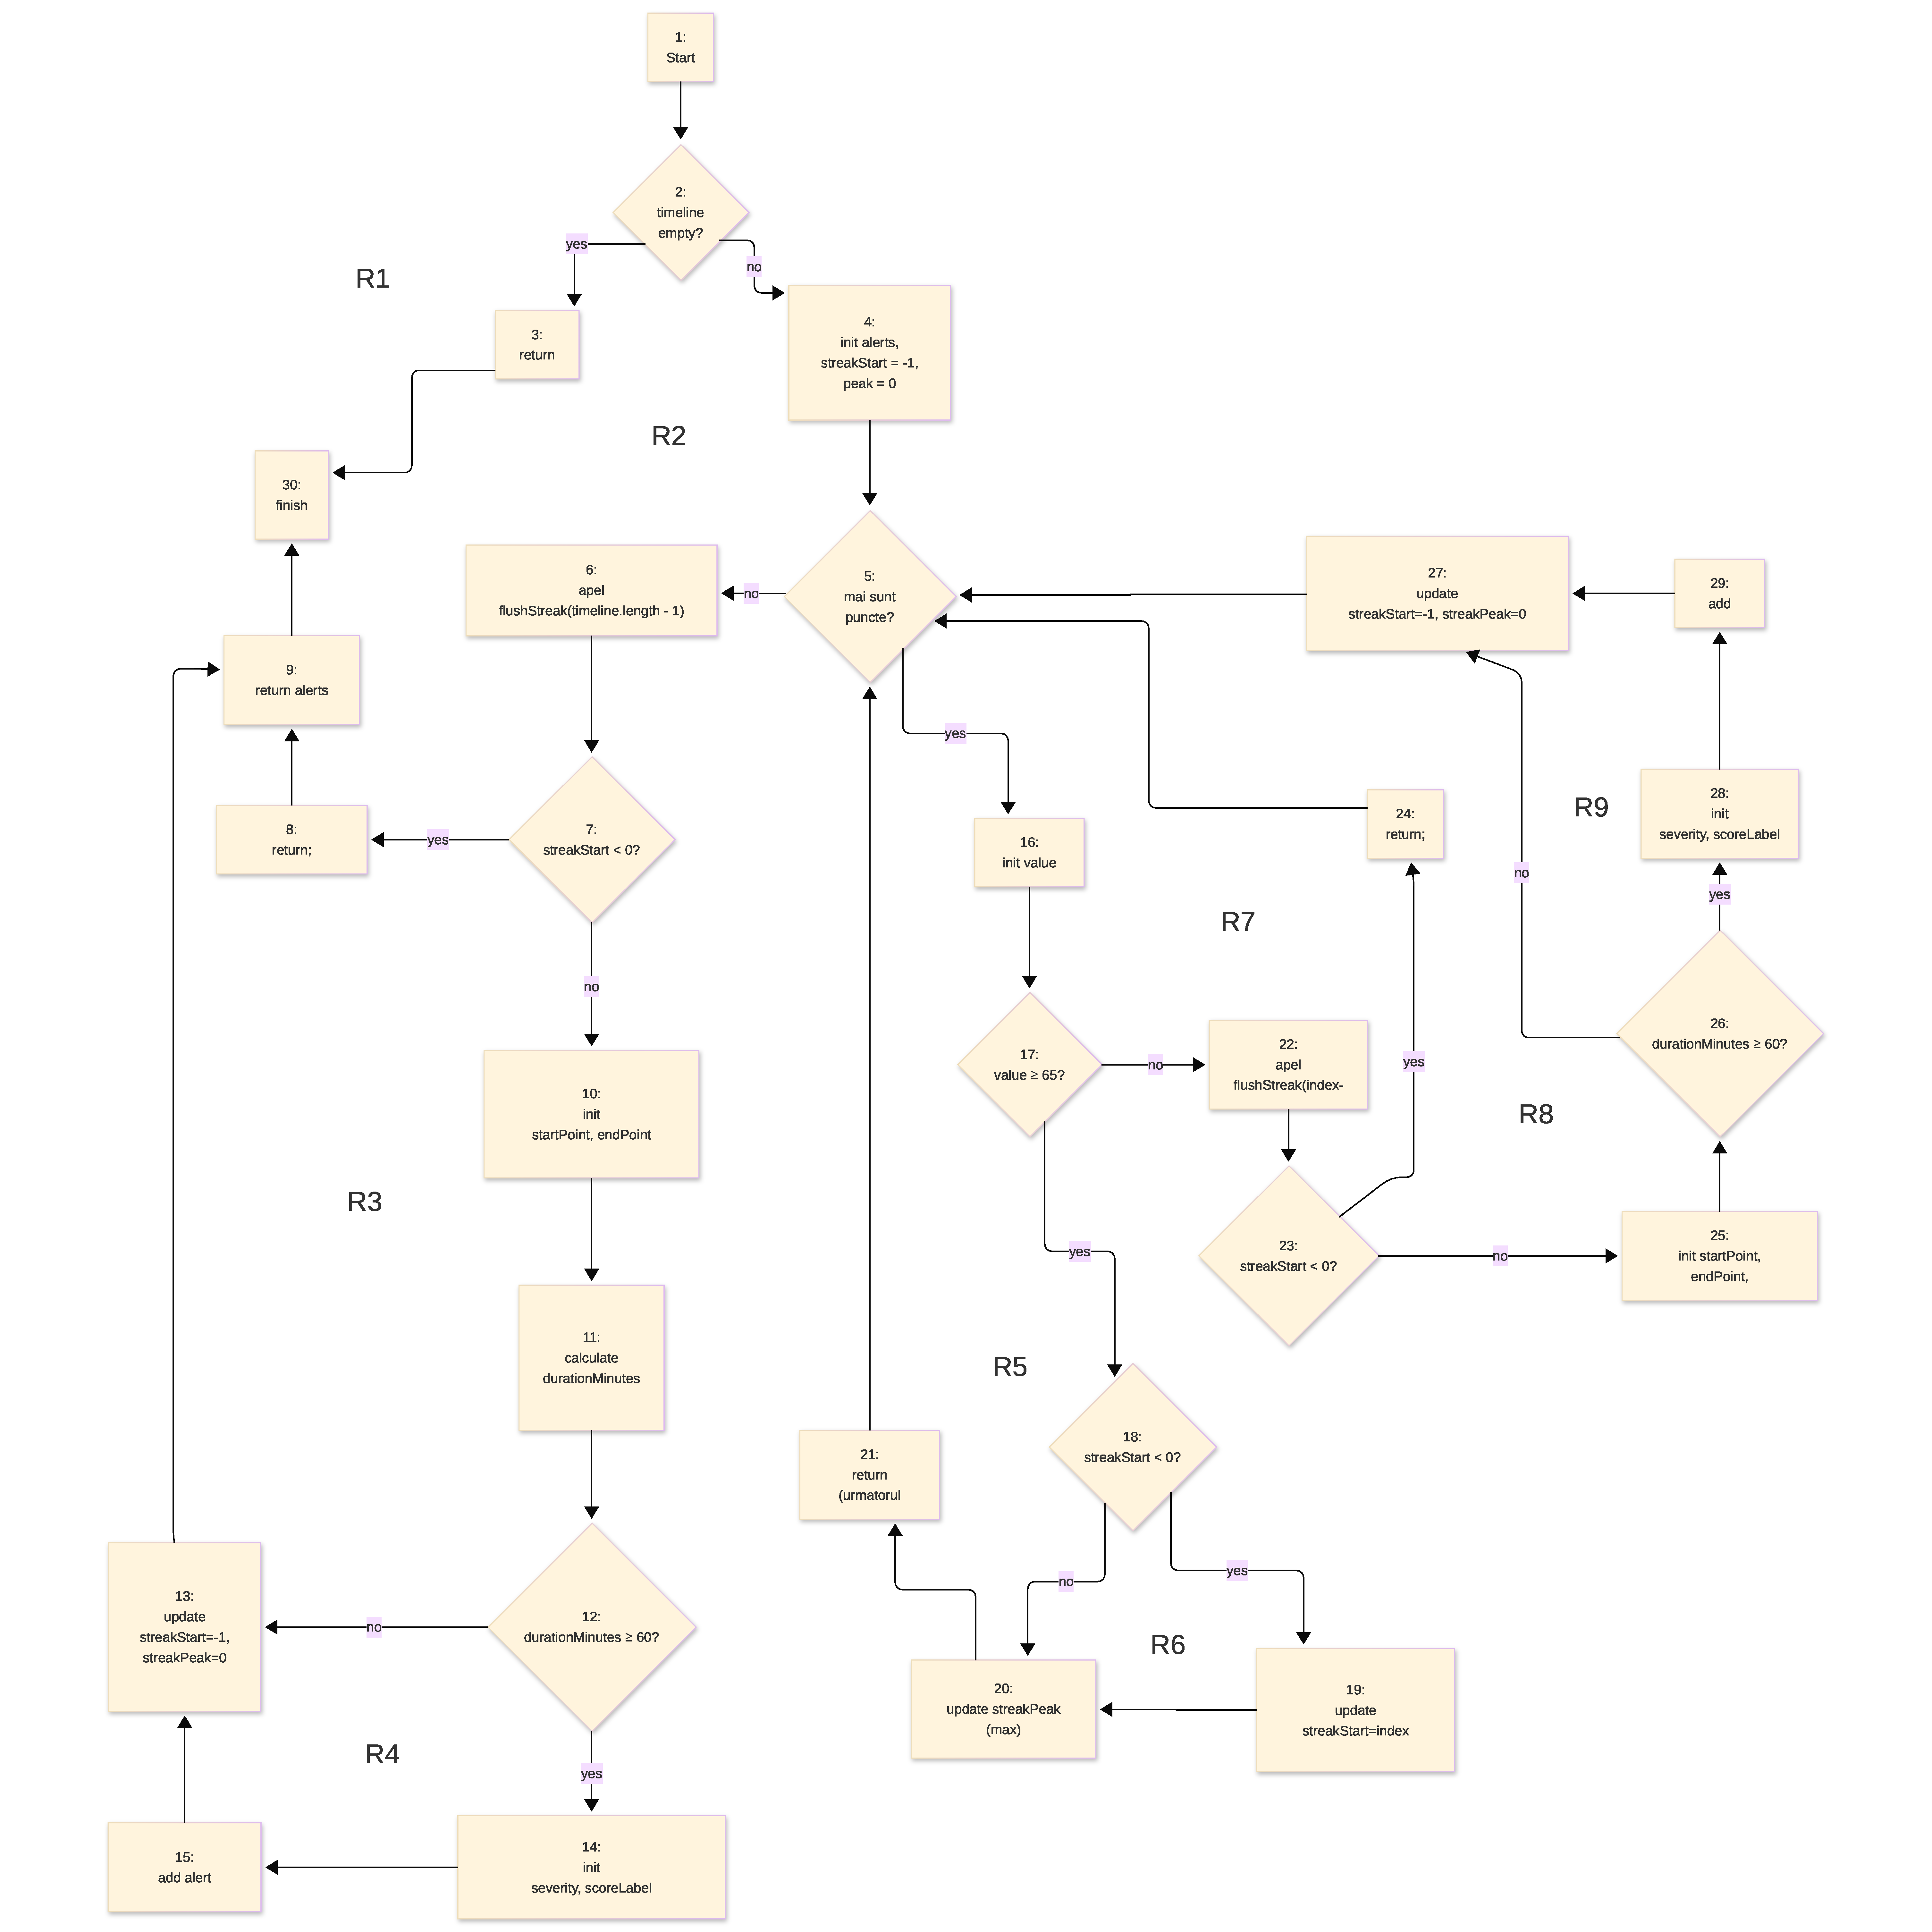
\includegraphics[width=0.97\textwidth]{figures/diagrams/cfg.pdf}
  \caption{CFG pentru \texttt{deriveProlongedAlert}.}
  \label{fig:cfg-derive-prolonged-alert}
\end{figure}

\noindent\textit{Nota:} pentru lizibilitate, apelul final \texttt{flushStreak(timeline.length - 1)} este comprimat in nodul \texttt{final flush}.

\subsubsection{Drumuri independente (set minim, CC=8)}
\begin{table}[htbp]
\centering
\footnotesize
\setlength{\tabcolsep}{5pt}
\renewcommand{\arraystretch}{1.15}
\begin{tabularx}{\textwidth}{p{0.9cm}p{3.6cm}p{4.9cm}X}
\toprule
\textbf{Path} & \textbf{Ramura noua acoperita} & \textbf{Date intrare (exemplu)} & \textbf{Rezultat asteptat} \\
\midrule
P1 & D1=True & \texttt{timeline=[]} & return lista vida, fara procesare. \\
P2 & D3=False + D5=True & toate valorile sub prag & fara alerta (nu exista streak activ). \\
P3 & D6=False & streak scurt (\(<60\) min) apoi intrerupere & fara alerta. \\
P4 & D6=True + D7=True & streak valid DISTRESS, durata \(\ge 60\) min & 1 alerta DISTRESS. \\
P5 & D6=True + D7=False & streak valid PAIN, durata \(\ge 60\) min & 1 alerta PAIN. \\
P6 & D4=False (streak continua) & mai multe puncte consecutive peste prag & streak mentinut corect, alerta unica la inchidere. \\
P7 & doua streak-uri mixte & primul \(<60\) min, al doilea \(\ge60\) min & exact 1 alerta (doar streak-ul valid). \\
P8 & inchidere prin \texttt{final flush} & streak activ la finalul listei & evaluare corecta la final (cu/fara alerta dupa durata). \\
\bottomrule
\end{tabularx}
\caption{Set compact de drumuri independente pentru acoperire basis-path.}
\label{tab:whitebox-compact-paths}
\end{table}

\section{Testarea de integrare}
\label{sec:testare-integrare}

\subsection{Scop}
Scopul testarii de integrare a fost validarea fluxului complet pentru endpoint-ul
\texttt{POST /api/doctor/patients/:patientId/readings}, de la nivel HTTP pana la nivel
controller/service si, in varianta extinsa, pana la persistenta reala in PostgreSQL.
S-au urmarit in special:
\begin{itemize}
  \item corectitudinea lantului \texttt{route -> middleware -> controller -> service};
  \item respectarea regulilor de autentificare si autorizare;
  \item persistenta corecta a citirilor emotionale;
  \item logica de alertare (creare alerta activa in scenarii de risc).
\end{itemize}

\subsection{Strategie}
Au fost implementate doua suite complementare:

\begin{itemize}
  \item \textbf{\texttt{doctor.readings.test.ts}}: integrare la nivel aplicatie (HTTP real prin \texttt{app}), cu infrastructura externa controlata prin mock (\texttt{Prisma}, \texttt{Influx}). Aceasta suita valideaza rapid fluxul functional si ramurile principale de business.
  \item \textbf{\texttt{doctor.readings.realdb.test.ts}}: integrare cu baza de date reala. Testul ruleaza pe schema dedicata \texttt{integration\_test}, aplica migrarile (\texttt{prisma migrate deploy}), face seed minim (\texttt{doctor/admin/ward/bed/patient}) si verifica efectiv datele scrise in PostgreSQL.
\end{itemize}

\subsection{Scenarii implementate}
\begin{table}[htbp]
\centering
\small
\setlength{\tabcolsep}{5pt}
\renewcommand{\arraystretch}{1.15}
\begin{tabularx}{\textwidth}{p{1.2cm}p{3.8cm}X p{2.0cm}}
\toprule
\textbf{ID} & \textbf{Suita} & \textbf{Scenariu} & \textbf{Rezultat} \\
\midrule
INT-01 & \texttt{doctor.readings.test.ts} &
Request fara header \texttt{Authorization} $\rightarrow$ raspuns \texttt{401}. &
Pass \\
INT-02 & \texttt{doctor.readings.test.ts} &
Token valid, dar rol \texttt{ADMIN} pe ruta de doctor $\rightarrow$ \texttt{403}. &
Pass \\
INT-03 & \texttt{doctor.readings.test.ts} &
Token \texttt{DOCTOR} valid + payload valid $\rightarrow$ \texttt{201}, apeluri corecte in service (\texttt{findUnique}, tranzactie, creare citire, logica alerta, apel Influx mock). &
Pass \\
\midrule
INT-04 & \texttt{doctor.readings.realdb.test.ts} &
Request fara \texttt{Authorization} in mediul cu DB real $\rightarrow$ \texttt{401}. &
Pass \\
INT-05 & \texttt{doctor.readings.realdb.test.ts} &
Token \texttt{ADMIN} pe ruta de doctor in mediul cu DB real $\rightarrow$ \texttt{403}. &
Pass \\
INT-06 & \texttt{doctor.readings.realdb.test.ts} &
Token \texttt{DOCTOR} valid + payload de risc ridicat $\rightarrow$ \texttt{201}; verificare in DB:
\texttt{EmotionReading} persistat + \texttt{PatientAlert} activ (tip \texttt{DISTRESS}, severitate corecta). &
Pass \\
\bottomrule
\end{tabularx}
\caption{Scenarii de integrare pentru endpoint-ul de readings.}
\label{tab:integration-readings}
\end{table}

\subsection{Mediu si executie}
Suita real-DB este controlata prin variabila de mediu \texttt{RUN\_DB\_INTEGRATION=1}.
Daca exista \texttt{DATABASE\_URL} in mediu, testul foloseste schema izolata
\texttt{integration\_test}; in lipsa acesteia, este prevazut fallback pe container PostgreSQL.

\noindent Comenzi de rulare:
\begin{verbatim}
# suita mock/full-app flow (rapid)
npm test --silent -- --runInBand --runTestsByPath src/__tests__/doctor.readings.test.ts

# suita cu baza reala (PowerShell)
$env:RUN_DB_INTEGRATION='1'
npm test --silent -- --runInBand --runTestsByPath src/__tests__/doctor.readings.realdb.test.ts
Remove-Item Env:RUN_DB_INTEGRATION
\end{verbatim}

\subsection{Rezultate obtinute}
La rularea curenta, ambele suite de integrare au trecut complet:
\begin{itemize}
  \item \texttt{doctor.readings.test.ts}: \textbf{3/3} teste trecute;
  \item \texttt{doctor.readings.realdb.test.ts}: \textbf{3/3} teste trecute;
  \item total integrare pe fluxul de readings: \textbf{6/6} teste trecute.
\end{itemize}

\subsection{Concluzie}
Prin combinarea suitei de integrare pe flux complet HTTP (cu dependinte externe controlate)
si a suitei de integrare cu persistenta reala, s-a obtinut un nivel bun de incredere asupra
functionalitatii endpoint-ului de readings: autentificarea/autorizarea, procesarea payload-ului,
persistenta datelor clinice si logica de alertare functioneaza corect in scenariile critice.


\section{Proiectare}
\subsection{Analiza cerințelor}
\subsection{Diagrama cazurilor de utilizare}
\subsection{Diagrame de interacțiune}
\section{Implementare}
\subsection{Server}
\subsection{Client}
\section{Testare}

\chapter{Concluzii}
%\chapter*{Concluzii}
\label{conclusions}

Prezenta lucrare a abordat optimizarea sistemelor de recunoaștere a emoțiilor faciale bazate pe rețele neuronale cu impulsuri prin preprocesare adaptivă, urmărind atât validarea potențialului SNN-urilor ca extractoare de trăsături spațio-temporale, cât și integrarea practică a unui motor de inferență a emoțiilor într-o aplicație clinică funcțională.

\section*{Sinteza concluziilor experimentale}

Evaluarea pe setul de date CK+ prin \textit{10-fold cross-validation} a confirmat că modelul CSNN 3D antrenat nesupervizat prin STDP extrage trăsături temporale relevante pentru clasificarea emoțiilor faciale. Rezultatele comparative obținute sunt sintetizate după cum urmează:

\begin{itemize}
	\item \textbf{Modelul CSNN 3D (propus):} Atinge cea mai mare acuratețe medie (de \textbf{56.10\%}) folosinf \textit{Random Sampler}, depășind clasificatorul de referință (SVM pe pixeli bruți, 36.57\%) cu un câștig net de \textbf{19.53\%}. Acest fapt demonstrează că nucleele convoluționale specializate prin STDP codifică corelații spațio-temporale discriminative. Deși contraintuitiv, \textit{Random Sampler} excelează raportat la celelalte tipuri de eșantionare (\textit{bounding-box}, \textit{landmark-centrată}, bazată pe \textit{activitatea neuronală}) deoarece asigură o distribuție nepolarizată a spike-urilor, prevenind supra-ajustarea (\textit{overfitting}) algoritmului STDP pe regiuni hiper-specifice și păstrând intacte dinamici temporale subtile care altfel ar fi fost filtrate.
	\item \textbf{Modelul ANN echivalent:} A obținut \textbf{75.97\%} (utilizând, însă, fețe decupate), cuantificând costul utilizării unei reguli de învățare locale și nesupervizate față de optimizarea globală prin gradient (\textit{backpropagation}).
	\item \textbf{Arhitectura CNN-LSTM:} Proiectată ca referință de tip \textit{upper bound}, a atins \textbf{88.37\% $\pm$ 5.65\%}, confirmând superioritatea transferului de cunoștințe (ResNet18) și a modelării explicite a dinamicii temporale.
\end{itemize}

Analiza hărților de trăsături a evidențiat că modelul SNN funcționează ca un extractor de trăsături fiziologice: emoțiile cu activare musculară intensă (\textit{Happiness, Surprise, Disgust}) au obținut un \textit{recall} cel puțin de \textbf{83\%} pe primul fold, în timp ce emoțiile subtile (\textit{Contempt, Sadness}) au condus la confuzii sistematice.

Experimentele au subliniat un avantaj structural al arhitecturii SNN: filtrul On/Off și codificarea prin latență oferă o robustețe nativă la zgomotul vizual. Pixelii statici din fundal nu generează impulsuri, spre deosebire de modelele ANN unde fundalul poate scădea acuratețea la aproximativ 30--40\% în absența decupării. Cele patru metode de eșantionare propuse constituie baza unei analize experimentale detaliate, în urma căreia \textit{Random Sampler} a ieșit câștigător.

\section*{Sistemul Neuro-Guardian}

Aplicația dezvoltată demonstrează viabilitatea integrării unui motor de inferență al emoțiilor într-un flux clinic real. Elementele cheie ale implementării includ:
\begin{itemize}
	\item \textbf{Arhitectura hibridă:} WebSocket pentru latență redusă, TCP pentru comunicarea cu serverul din Python, PostgreSQL pentru date clinice și InfluxDB pentru monitorizarea seriilor temporale ale emoțiilor.
	\item \textbf{Mecanismul de histerezis:} Utilizarea pragurilor \textit{70/55} pentru alertele de tip \textit{Distress} și \textit{Pain} elimină oscilațiile la pragurile de decizie, oferind notificări stabile.
	\item \textbf{Validare complexă:} Combinarea testării \textit{white-box} (9 drumuri independente, Complexitate Ciclomatică = 9) cu integrarea \textit{top-down depth-first} realizată prin \textit{Jest}, \textit{Supertest} și \textit{Testcontainers} pentru izolarea dependențelor reale asigură o testare robustă a aplicației. 
\end{itemize}

\section*{Limitări și direcții viitoare de cercetare}

Lucrarea prezintă câteva limitări inerente:
\begin{enumerate}
	\item \textbf{Setul de date:} CK+ este colectat în condiții controlate, ceea ce poate limita generalizarea la emoții spontane.
	\item \textbf{Dezechilibrul claselor:} Numărul redus de exemple pentru \textit{Contempt} și \textit{Fear} afectează negativ performanța, STDP prioritizând trăsăturile frecvente.
	\item \textbf{Hardware:} Modelul rulează pe hardware convențional, beneficiile energetice ale SNN fiind maximizate doar pe cipuri precum Intel Loihi.
\end{enumerate}

Pe baza rezultatelor obținute, se propun următoarele direcții de extindere:
\begin{itemize}
	\item \textbf{Optimizarea altor hiperparametrilor:} Rafinarea pragului de activare ($\theta$) și a ratei de învățare ($\mu_{th}$) prin optimizare bayesiană.
	\item \textbf{Codificare temporală:} Înlocuirea \textit{latency coding} cu alte metode de codificare la nivelul întregii arhitecturi.
	\item \textbf{Antrenare End-to-End:} Implementarea unui strat \textit{Fully Connected Spiking} antrenat fie prin \textit{surrogate gradients}, fie prin STDP pentru a elimina necesitatea unui SVM extern.
	\item \textbf{Analiza robusteții:} Antrenarea și testarea arhitecturii și pe alte seturi de date mai complexe, cu mai mult zgomot de fundal.
\end{itemize}

În concluzie, lucrarea demonstrează că rețelele neuronale cu impulsuri sunt capabile să extragă trăsături relevante chiar și în regim nesupervizat, deschizând perspective reale pentru sisteme de recunoaștere a emoțiilor eficiente energetic, de tip \textit{Edge AI}.

%\addcontentsline{toc}{chapter}{Concluzii}
%\addcontentsline{toc}{chapter}{Conclusions}

\bibliography{references}

\end{document}
